\chapter{Observaties}
In dit hoofdstuk worden de resultaten getoond van de testen die zijn uitgevoerd. Deze resultaten zullen in dit hoofdstuk enkel getoond worden met een bespreking van de speciale elementen. Er zullen nog geen conclusies gemaakt worden, dit wordt in het volgende hoofdstuk gedaan. 

De resultaten zullen besproken worden per testsoort: eerst de resultaten voor de calibratie daarna voor beschikbaarheid en tenslotte voor consistentie. 

De ruwe testdata kan geraadpleegd worden op \url{https://github.com/thuys/YCSB-Testdata}. 

\section{Calibratie}

\paragraph{Aantal gebruikers}
De resultaten van de calibratietest voor het aantal gebruikers kunnen gevonden worden in figuur \ref{fig:calibratie-gebruikers-resultaat}. Op de x-as is het gemiddeld aantal queries per second getoond over een periode van 600s, op de y-as de gemiddelde vertraging. De verschillende punten stellen een aantal gebruikers voor die zijn aangegeven met het bijhorend getal. 

Het aantal gebruikers wordt zo gekozen dat het totale aantal queries zakt of voor een sterke groei in vertraging zorgt, dit zorgt voor de gegevens in tabel \ref{table:calibratie-gebruikers-resultaat}. Bij MongoDB is er voor een lage waarde van 15 gebruikers gekozen, in plaats van 50, de reden hiervoor is dat de variatie in de vertraging groter wordt bij meer gebruikers, wat de testen moeilijker maakt.  

\begin{table}[h!]
	\centering
	\begin{tabular}{l| l }
		\textbf{DBMS} & Aantal gebruikers \\
		\hline
		HBase & 50 \\
		MongoDB & 15\\
		Pgpool-II & 30\\
	\end{tabular}
	\caption{Calibratie: Aantal gebruikers per test voor de verschillende DBMS's}
	\label{table:calibratie-gebruikers-resultaat}
\end{table}

\begin{figure}[h!] 
\centering
	\subfigure[MongoDB]{\label{fig:calibratie-gebruikers-mongodb} \includegraphics[width=0.4\textwidth]{img/Observaties/threads-MongoDB}}
	\subfigure[Pgpool-II]{\label{fig:calibratie-gebruikers-pgpool-ii} 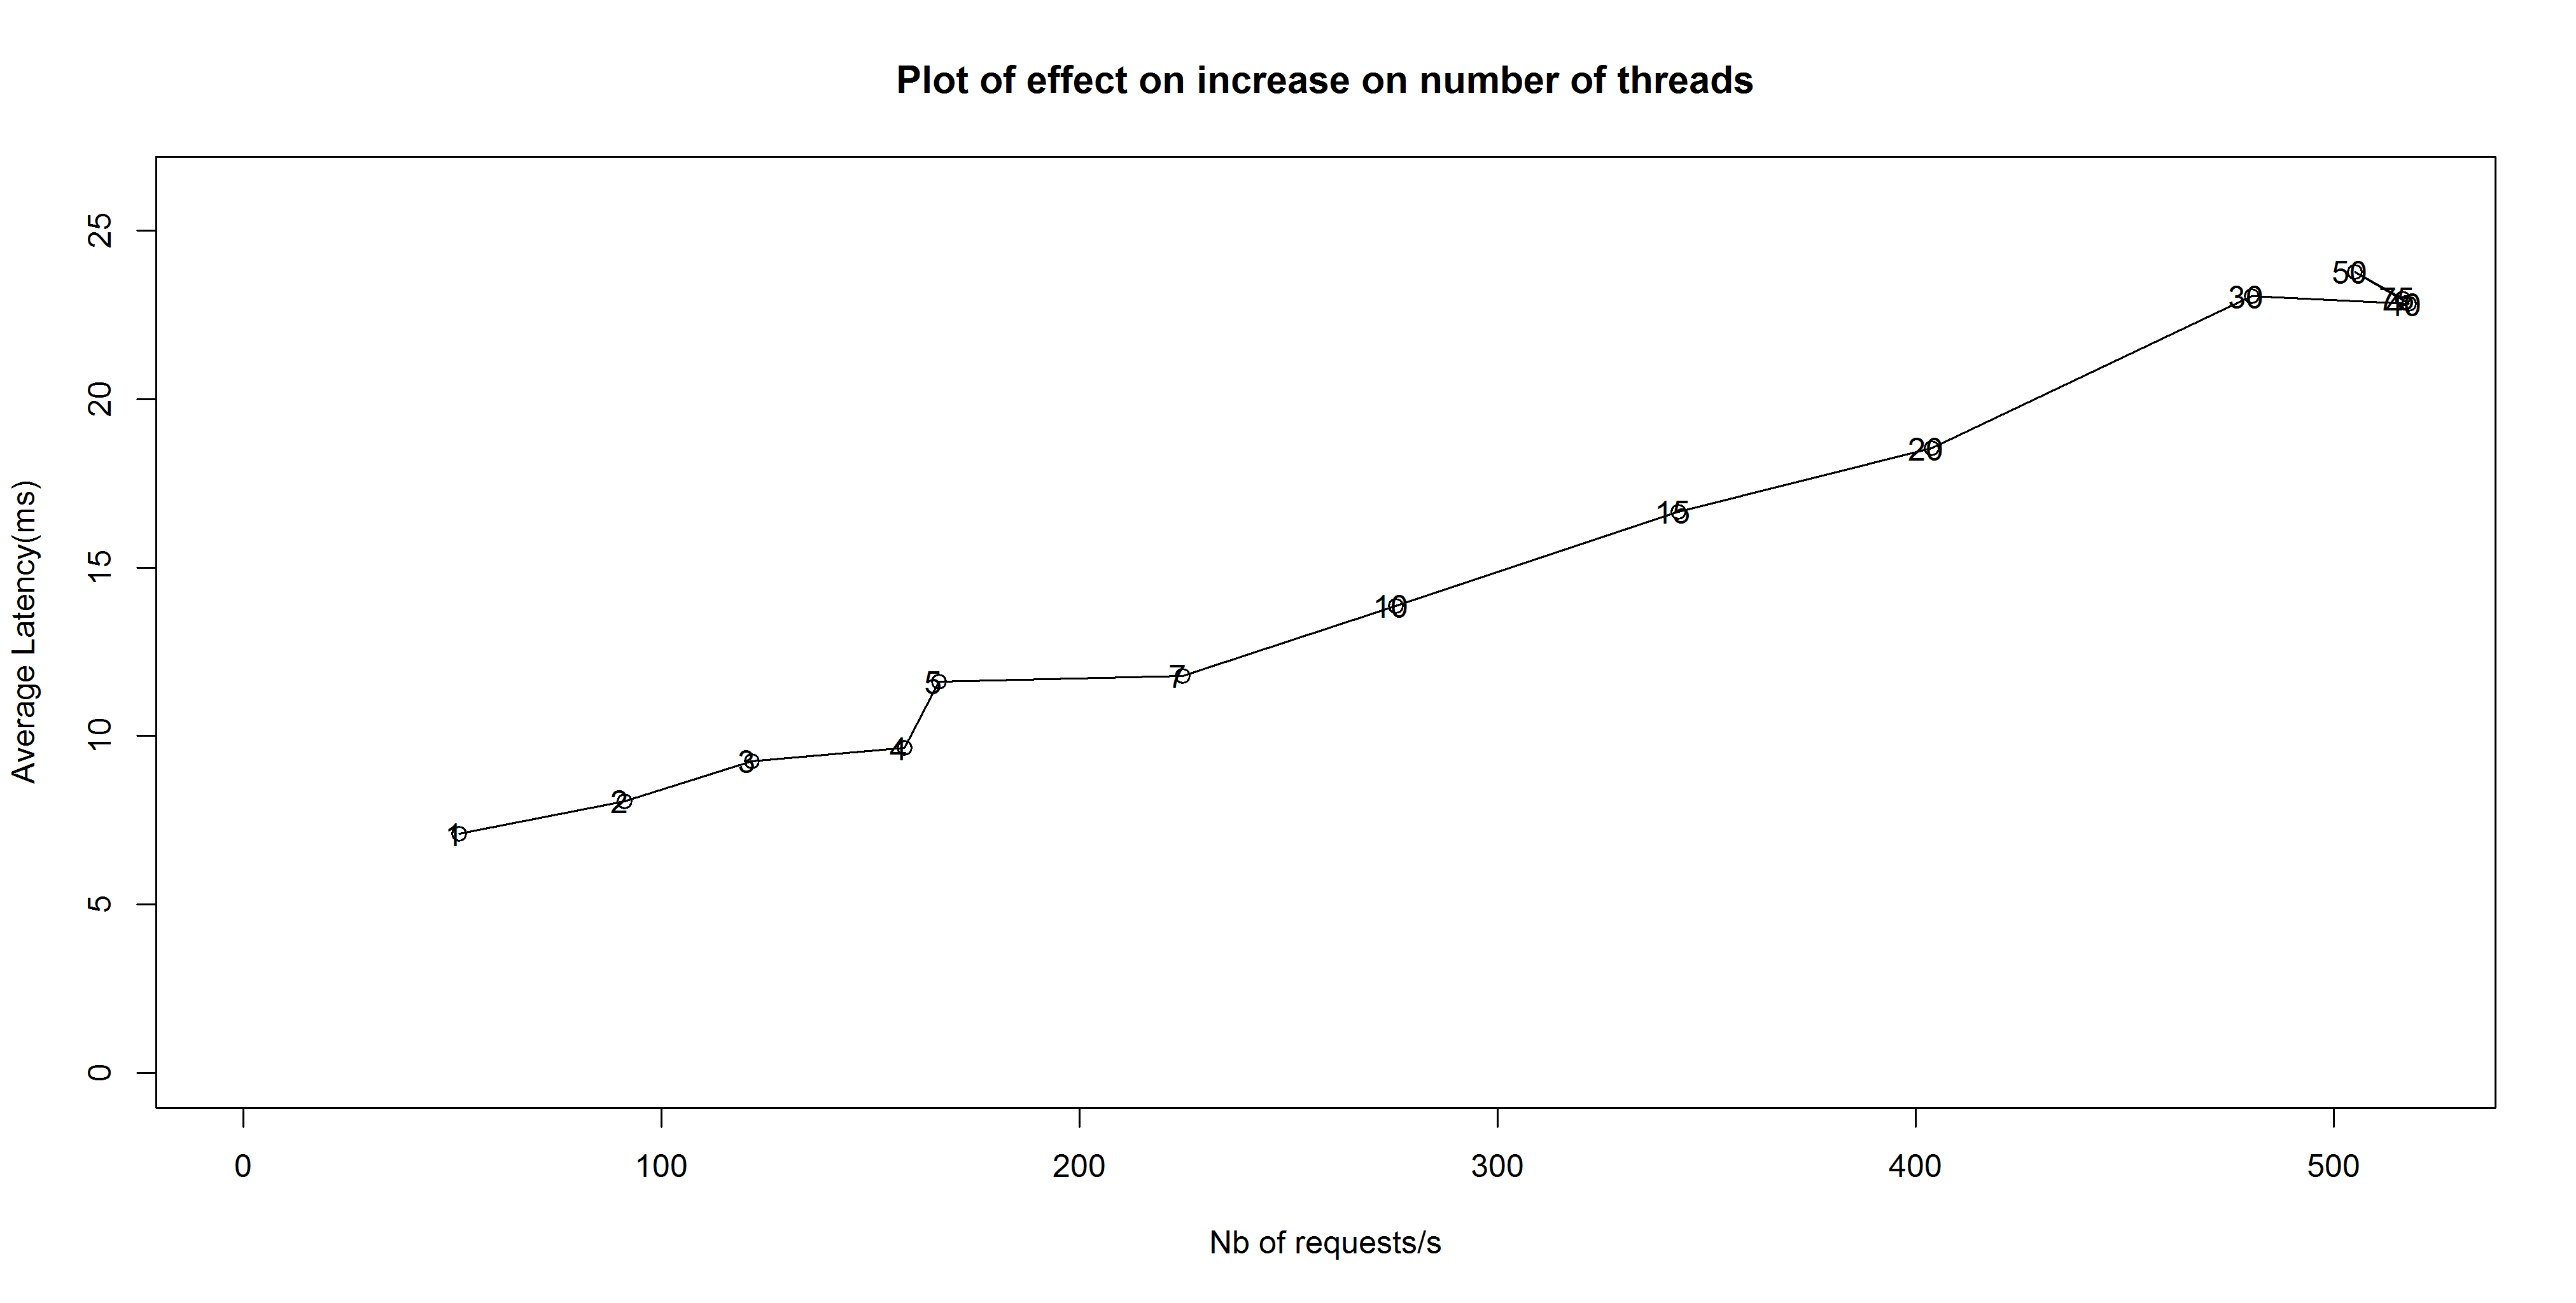
\includegraphics[width=0.4\textwidth]{img/Observaties/threads-postgresql}}
	\subfigure[HBase]{\label{fig:calibratie-gebruikers-hbase} \includegraphics[width=0.4\textwidth]{img/Observaties/threads-HBase}}
	\caption{Calibratie: Overzicht van het aantal queries tot de gemiddelde vertraging voor verschillend aantal gebruikers. Elk datapunt stelt een verschillend aantal gebruikers voor met het aantal rechtsboven het punt. }
	\label{fig:calibratie-gebruikers-resultaat}
\end{figure}

\paragraph{Aantal queries per seconde}
De resultaten voor de calibratietest voor het aantal queries per seconden kunnen gevonden worden in de figuren \ref{fig:calibratie-queriesperseconde-hbase}, \ref{fig:calibratie-queriesperseconde-mongodb} en \ref{fig:calibratie-queriesperseconde-pgpool-ii} voor respectievelijk HBase, MongoDB en Pgpool-II. Deze figuren tonen in de bovenste figuur de gemiddelde vertraging op een query afhankelijk van het aantal queries per seconde, zoals te verwachten stijgt de trendlijn hierdoor. De onderste figuur toont op de y-as de verhouding tussen het eigenlijk aantal uitgevoerde queries per seconde t.o.v. het gevraagde aantal queries per seconde. Bij het vragen van 100 queries/sec wordt er in de praktijk bijvoorbeeld maar 60 uitgevoerd, dit zorgt voor een waarde $0.6$. 

Met beide figuren samen, kan een matige belasting gekozen. Een matige belasting is een belasting waarbij de onderste figuur de waarde 1 zo dicht mogelijk benaderd en de vertraging nog niet te veel is gestegen t.o.v. van een lage belasting. De gekozen waarde zijn te vinden in tabel \ref{table:calibratie-queriesperseconde-resultaat}. 

\begin{table}[h!]
	\centering
	\begin{tabular}{l| l }
		\textbf{DBMS} & Aantal requests per seconde \\
		\hline
		HBase & 600 \\
		MongoDB & 200\\
		Pgpool-II & 100\\
	\end{tabular}
	\caption{Calibratie: Aantal queries per seconde per test bij een matige belasting voor de verschillende DBMS's.}
	\label{table:calibratie-queriesperseconde-resultaat}
\end{table}

\begin{figure}[h!] 
	\centering
	\subfigure{\label{fig:calibratie-queriesperseconde-hbase-1} 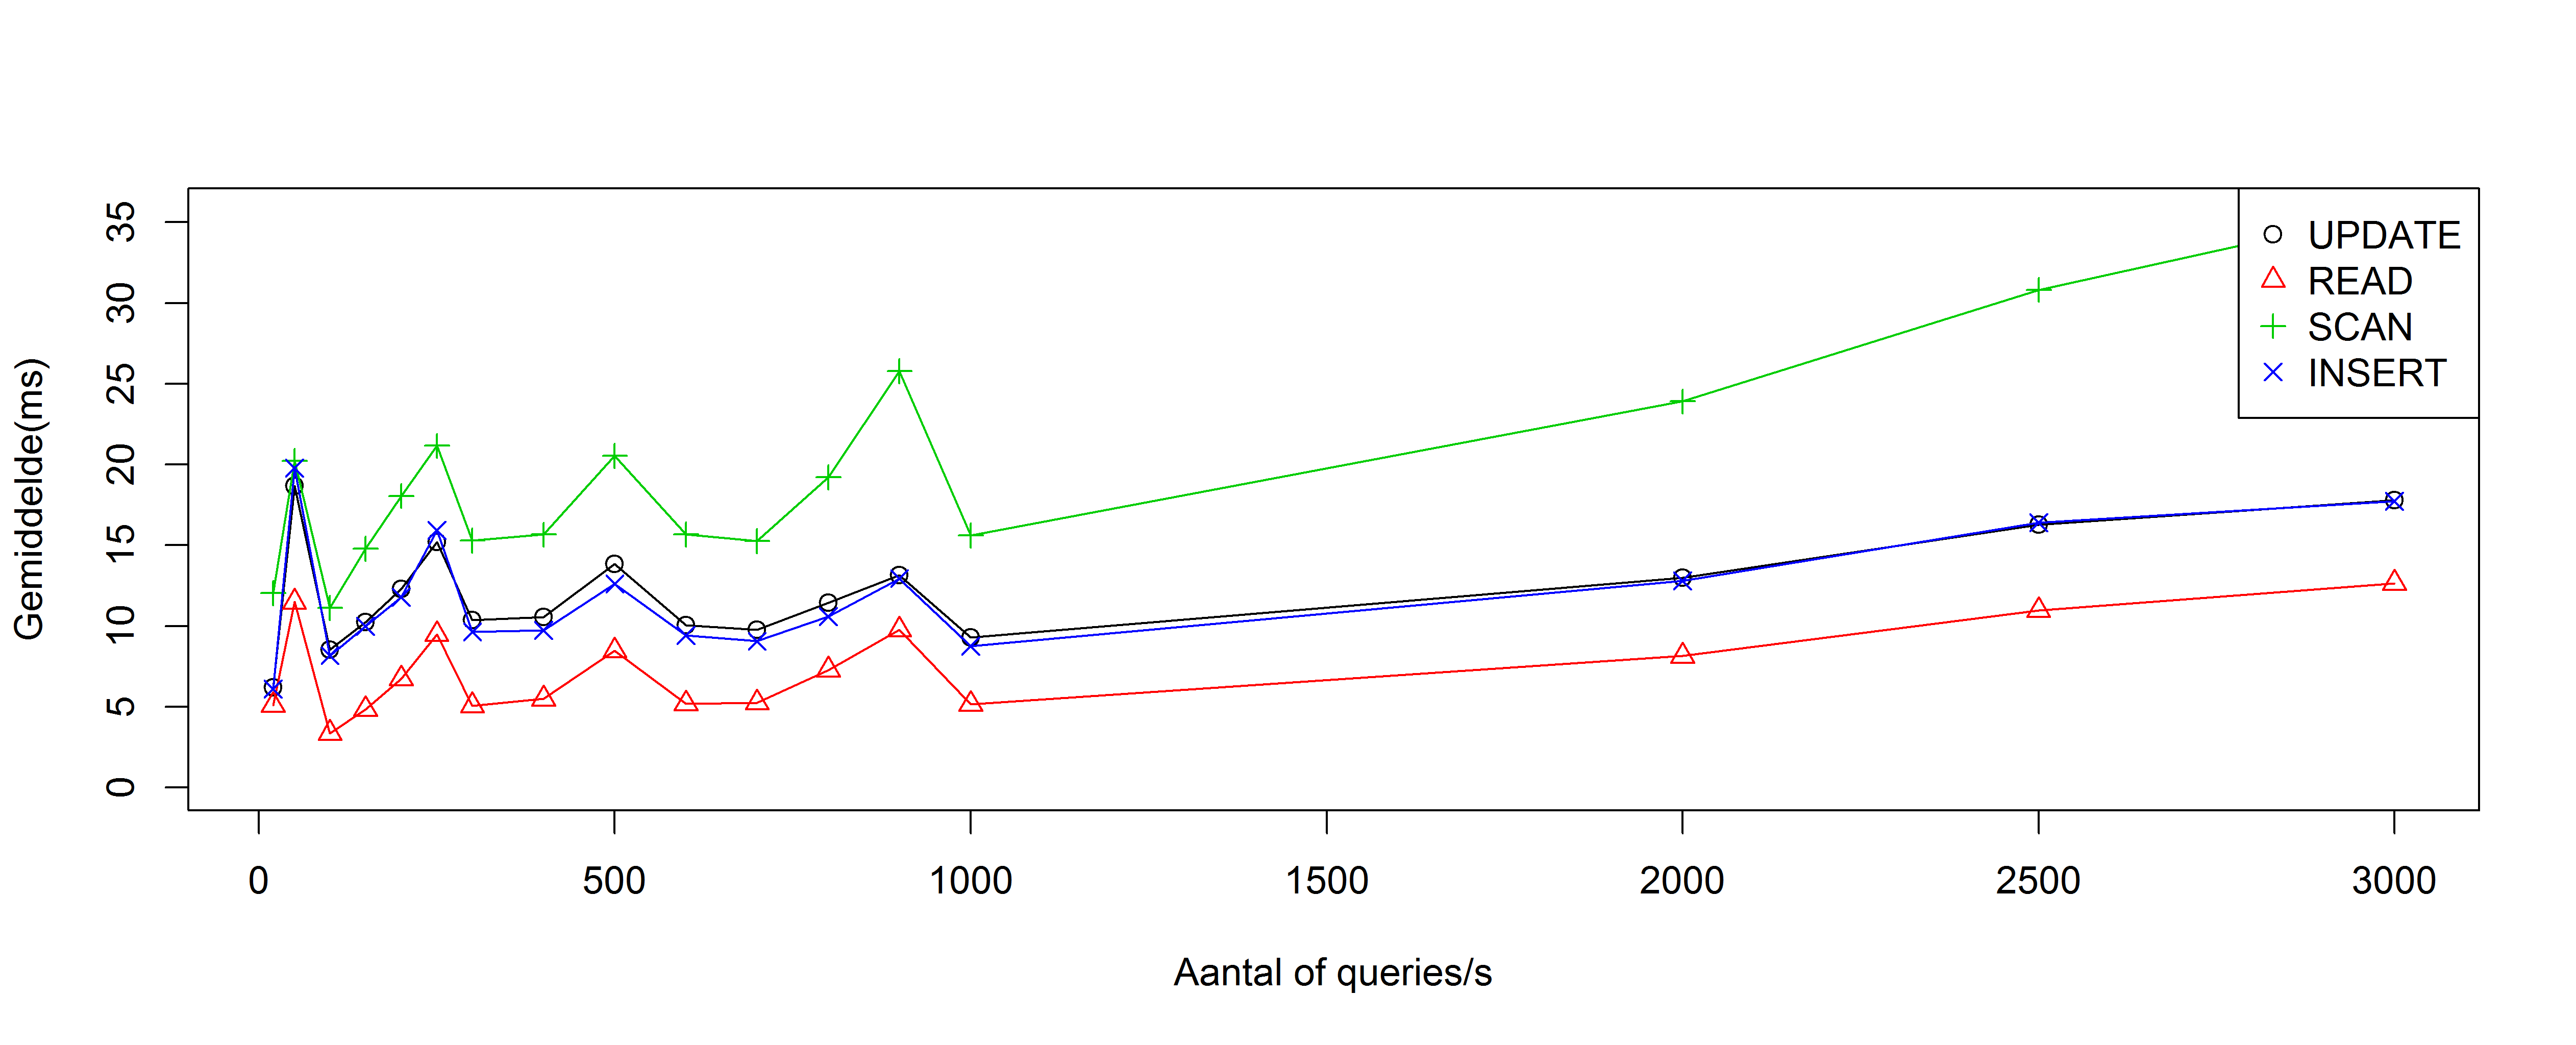
\includegraphics[width=\textwidth]{img/Observaties/loadbalance-db-HBase}}
	\subfigure{\label{fig:calibratie-queriesperseconde-hbase-2} 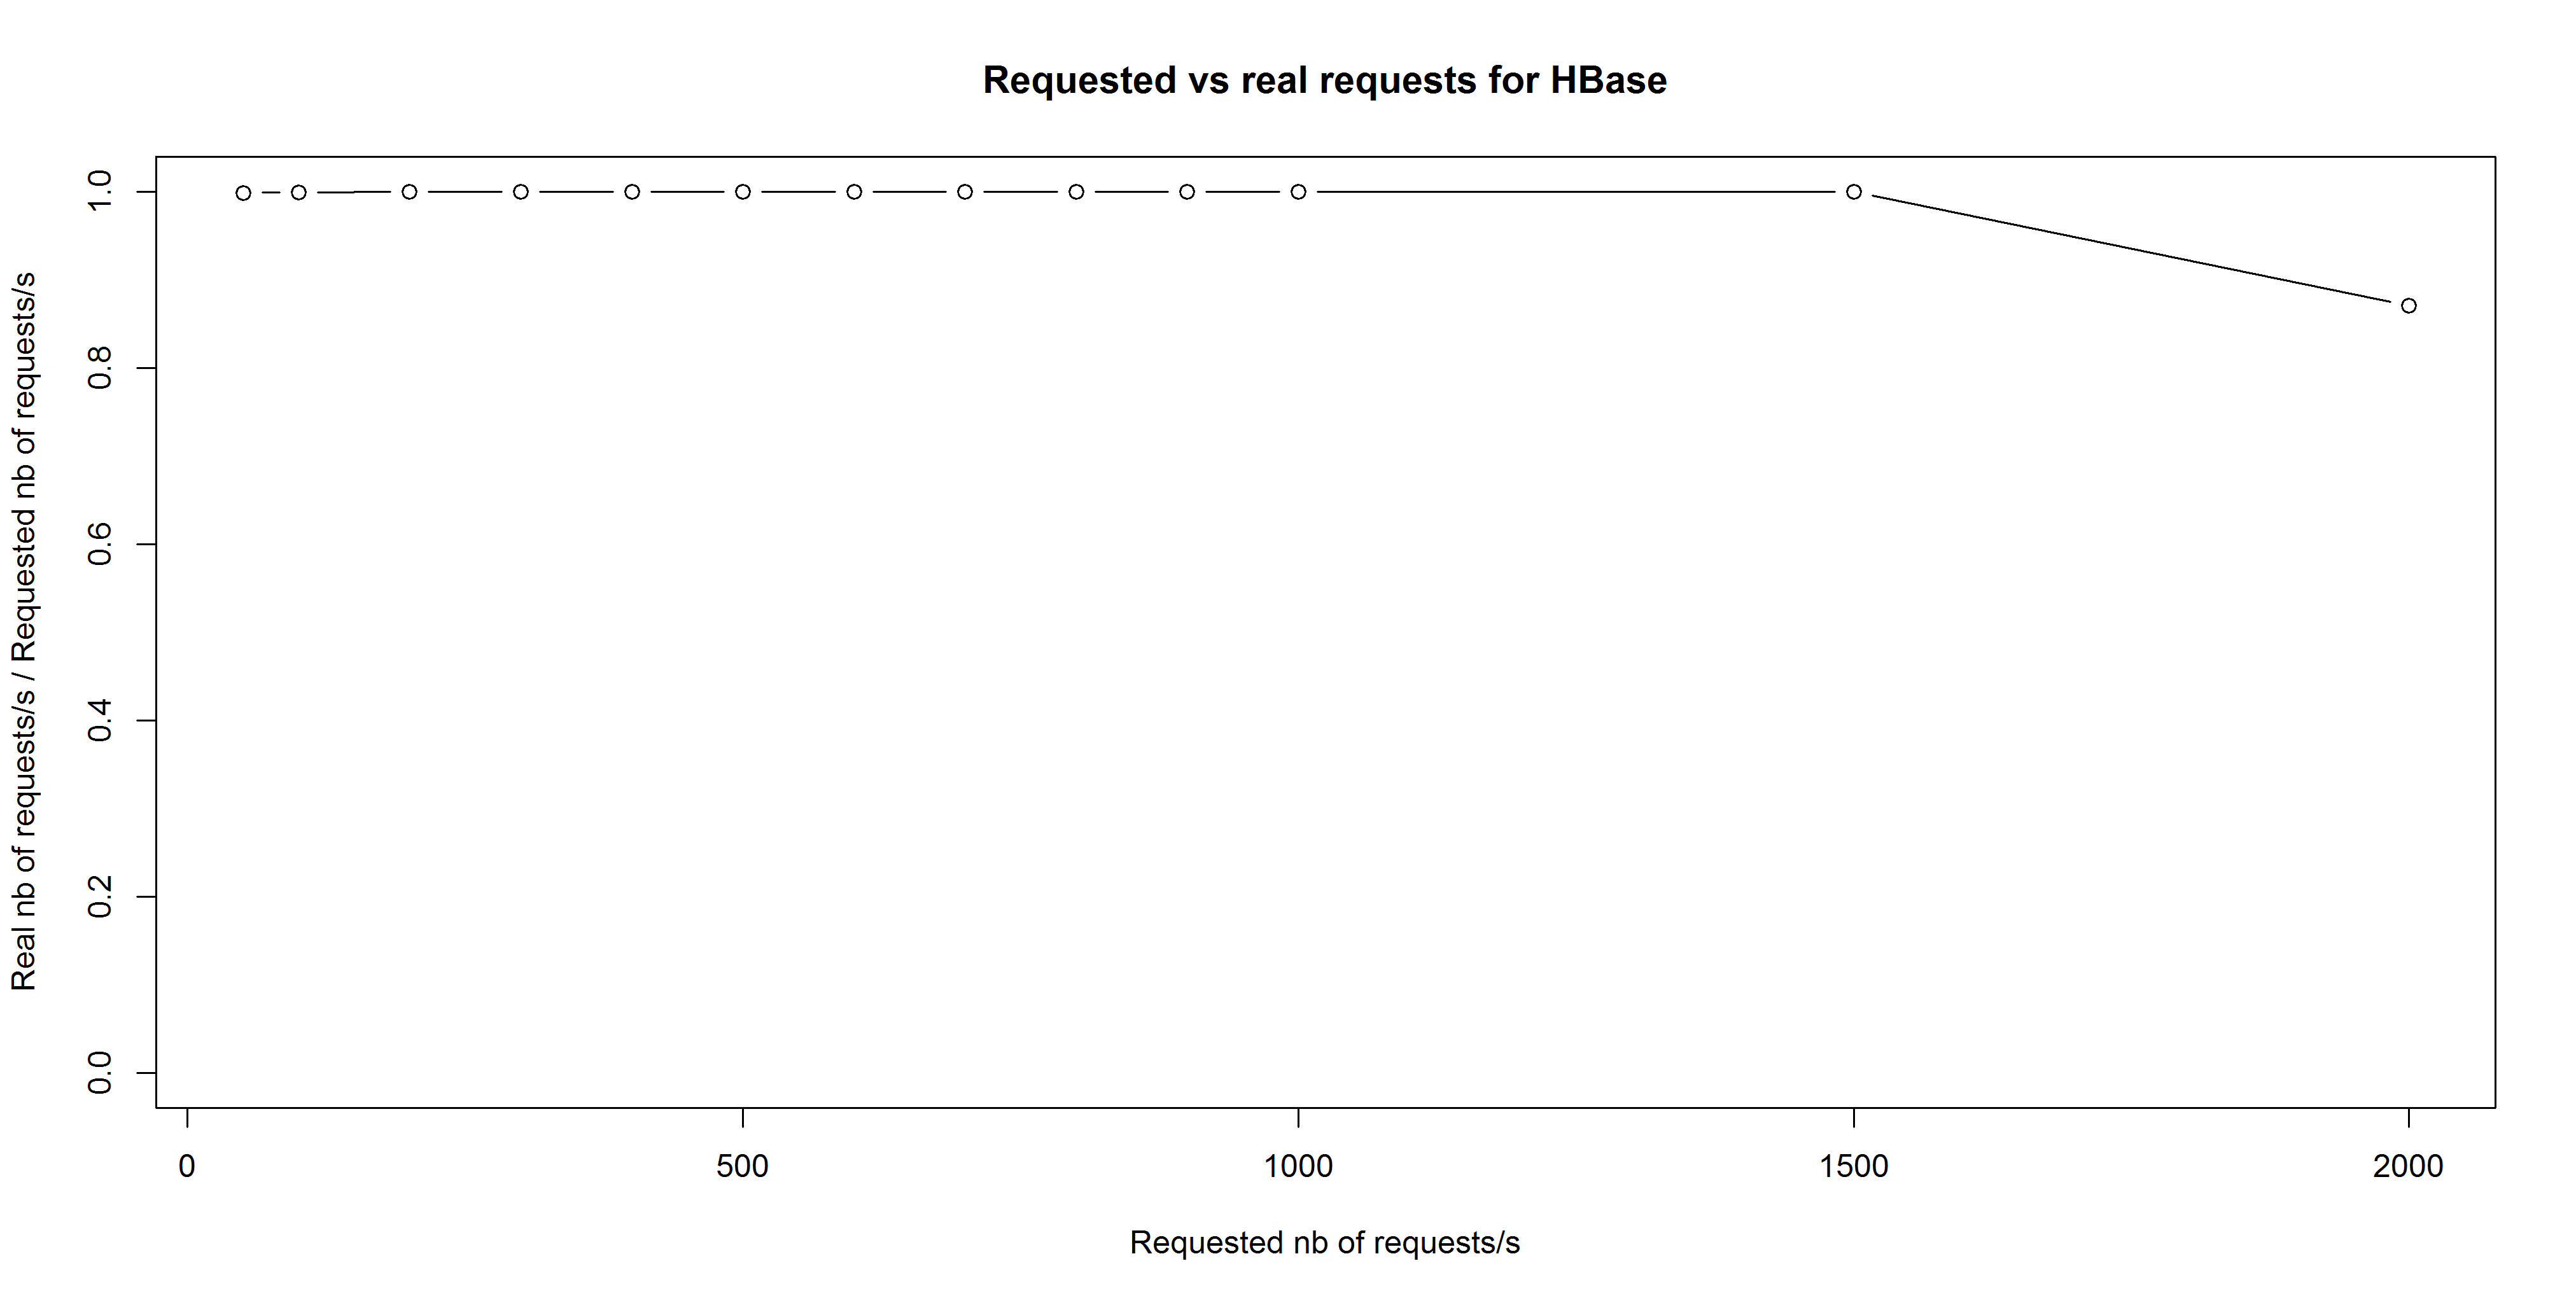
\includegraphics[width=\textwidth]{img/Observaties/loadbalance-realthroughput-db-HBase}}
	\caption{Calibratie: Overzicht van de vertraging t.o.v. het theoretisch aantal aanvragen met een vergelijking hoeveel werkelijke aanvragen er waren voor HBase. }
	\label{fig:calibratie-queriesperseconde-hbase}
\end{figure}

\begin{figure}[h!] 
	\centering
	\subfigure{\label{fig:calibratie-queriesperseconde-mongodb-1} 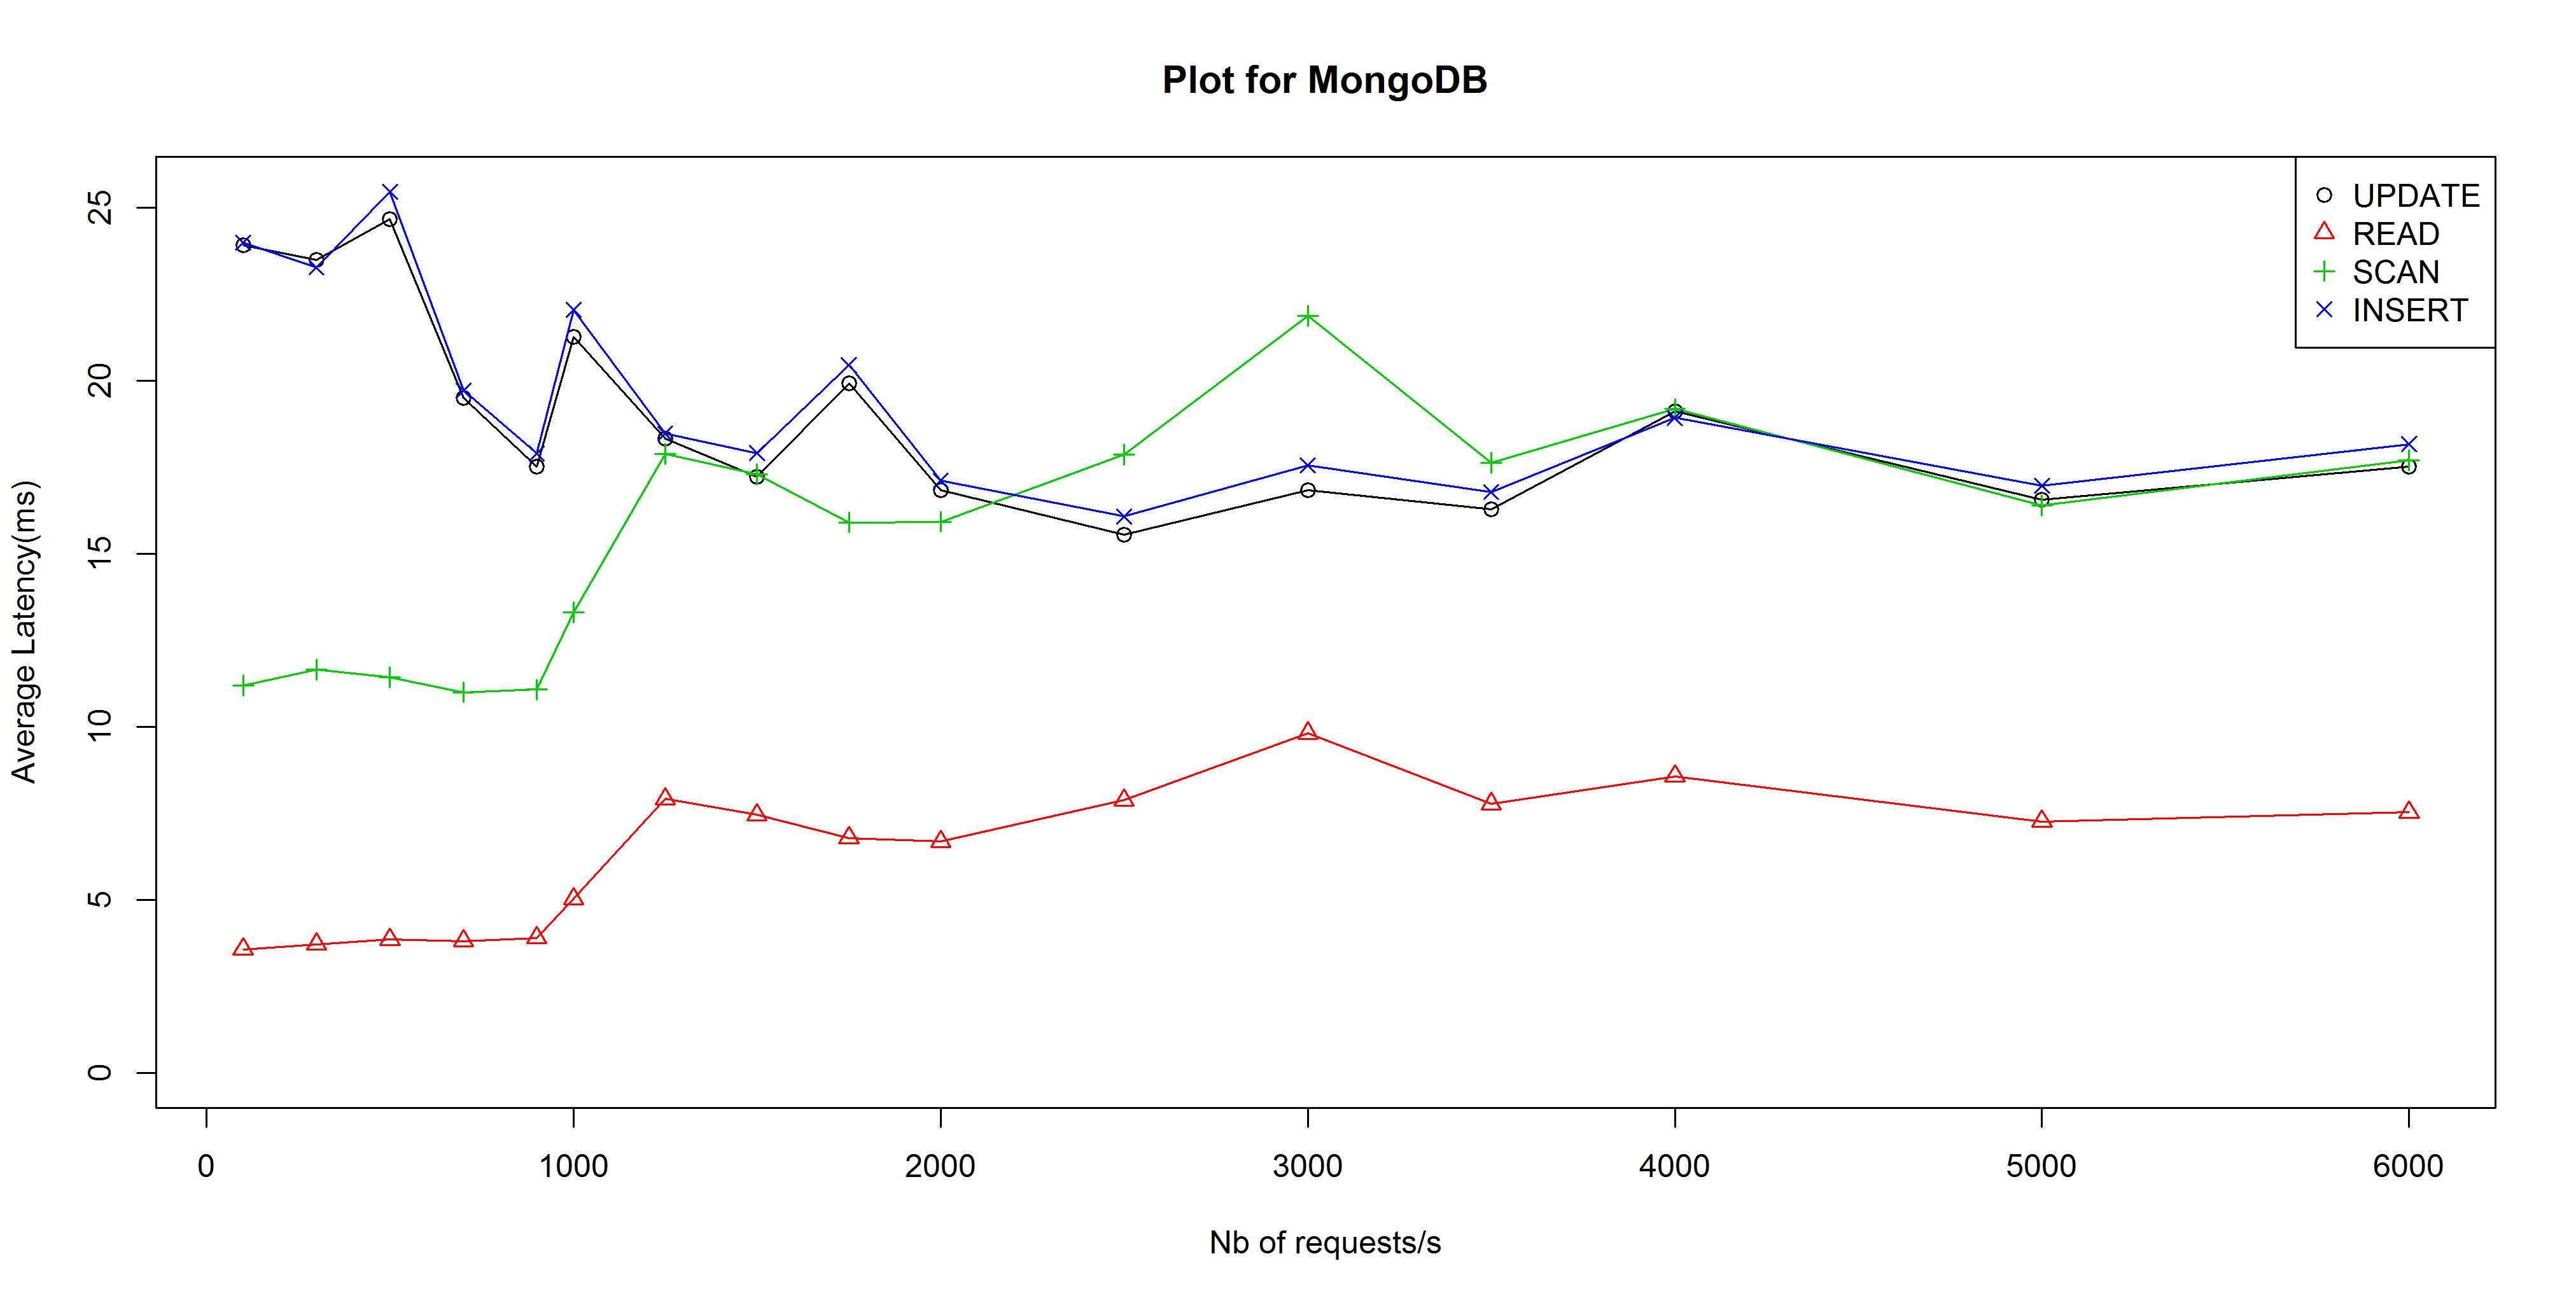
\includegraphics[width=\textwidth]{img/Observaties/loadbalance-db-MongoDB}}
	\subfigure{\label{fig:calibratie-queriesperseconde-mongodb-2} 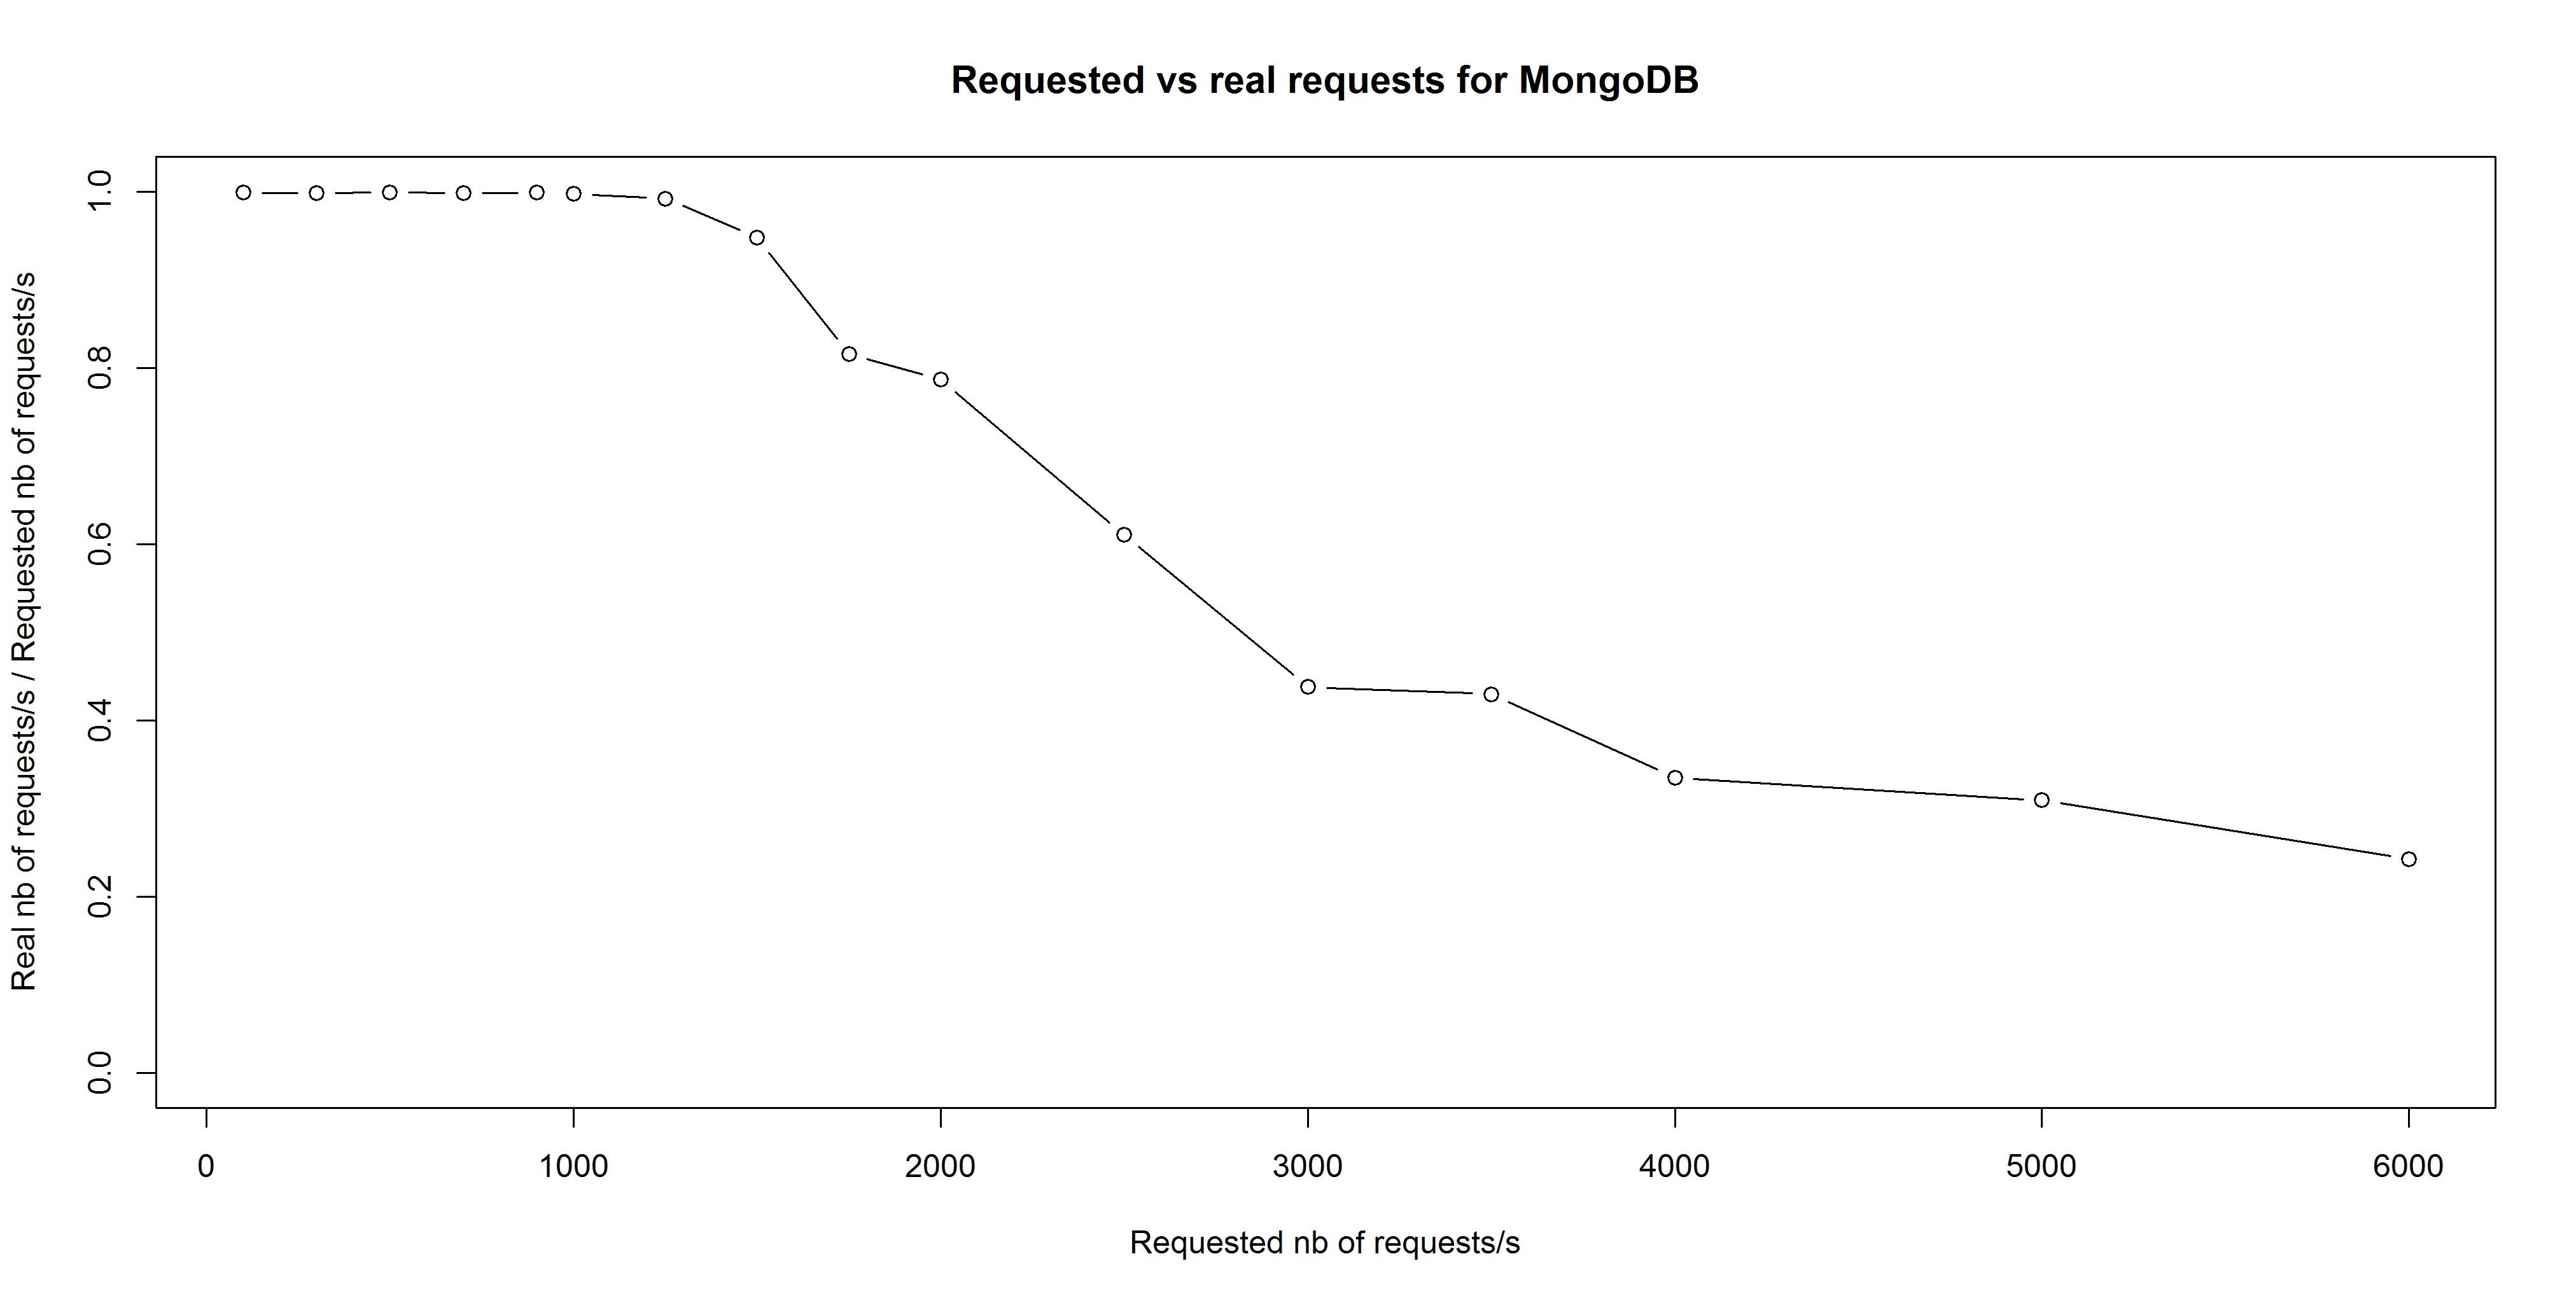
\includegraphics[width=\textwidth]{img/Observaties/loadbalance-realthroughput-db-MongoDB}}
	\caption{Calibratie: Overzicht van de vertraging t.o.v. het theoretisch aantal aanvragen met een vergelijking hoeveel werkelijke aanvragen er waren voor MongoDB. }
	\label{fig:calibratie-queriesperseconde-mongodb}
\end{figure}

\begin{figure}[h!] 
	\centering
	\subfigure{\label{fig:calibratie-queriesperseconde-pgpool-ii-1} 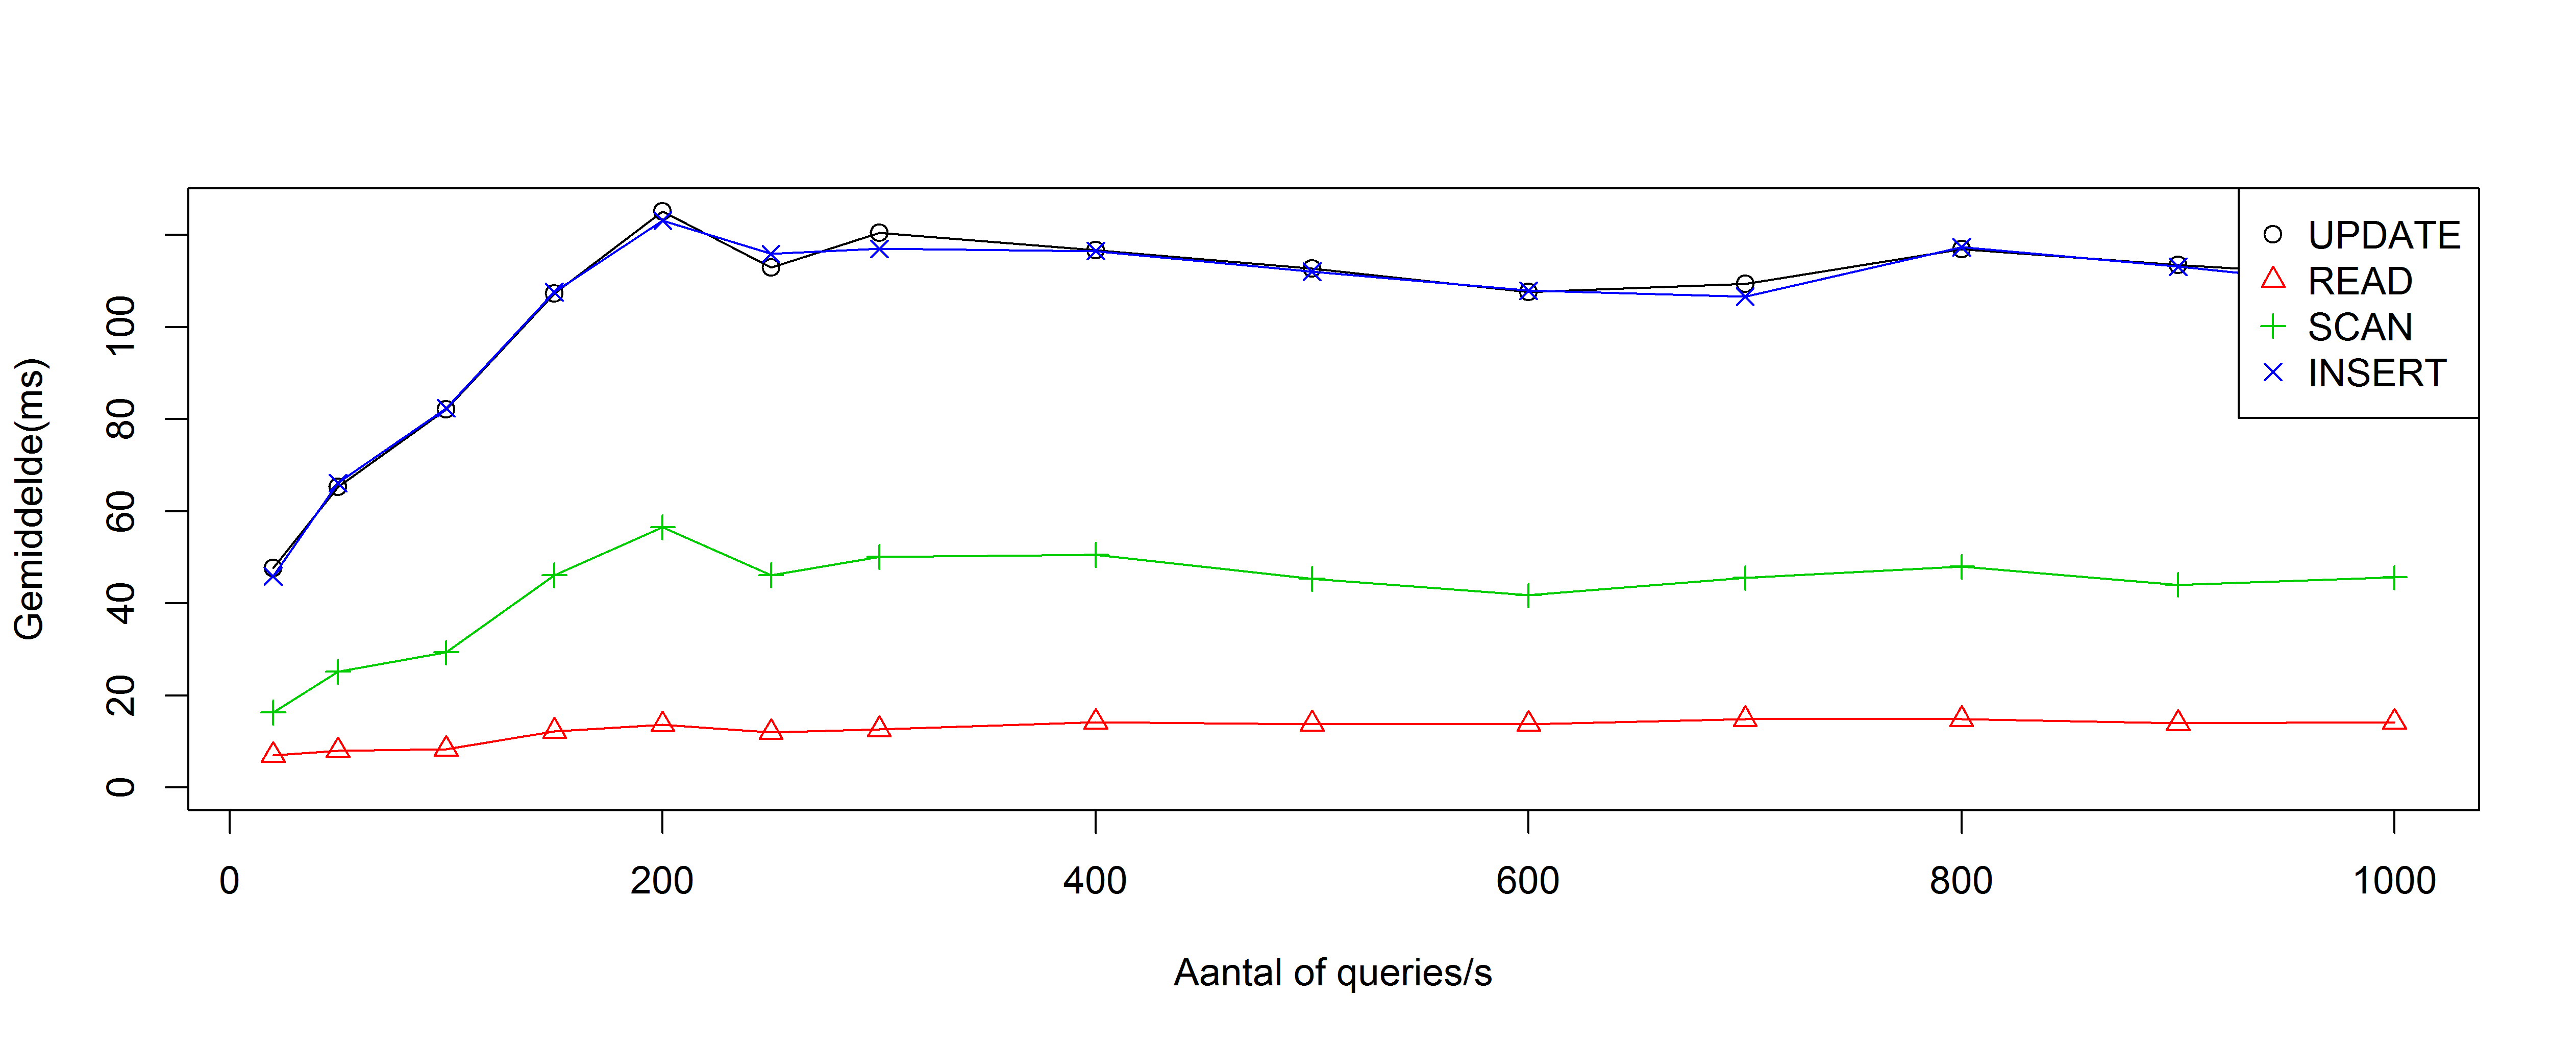
\includegraphics[width=\textwidth]{img/Observaties/loadbalance-db-PostgreSQL}}
	\subfigure{\label{fig:calibratie-queriesperseconde-pgpool-ii-2} 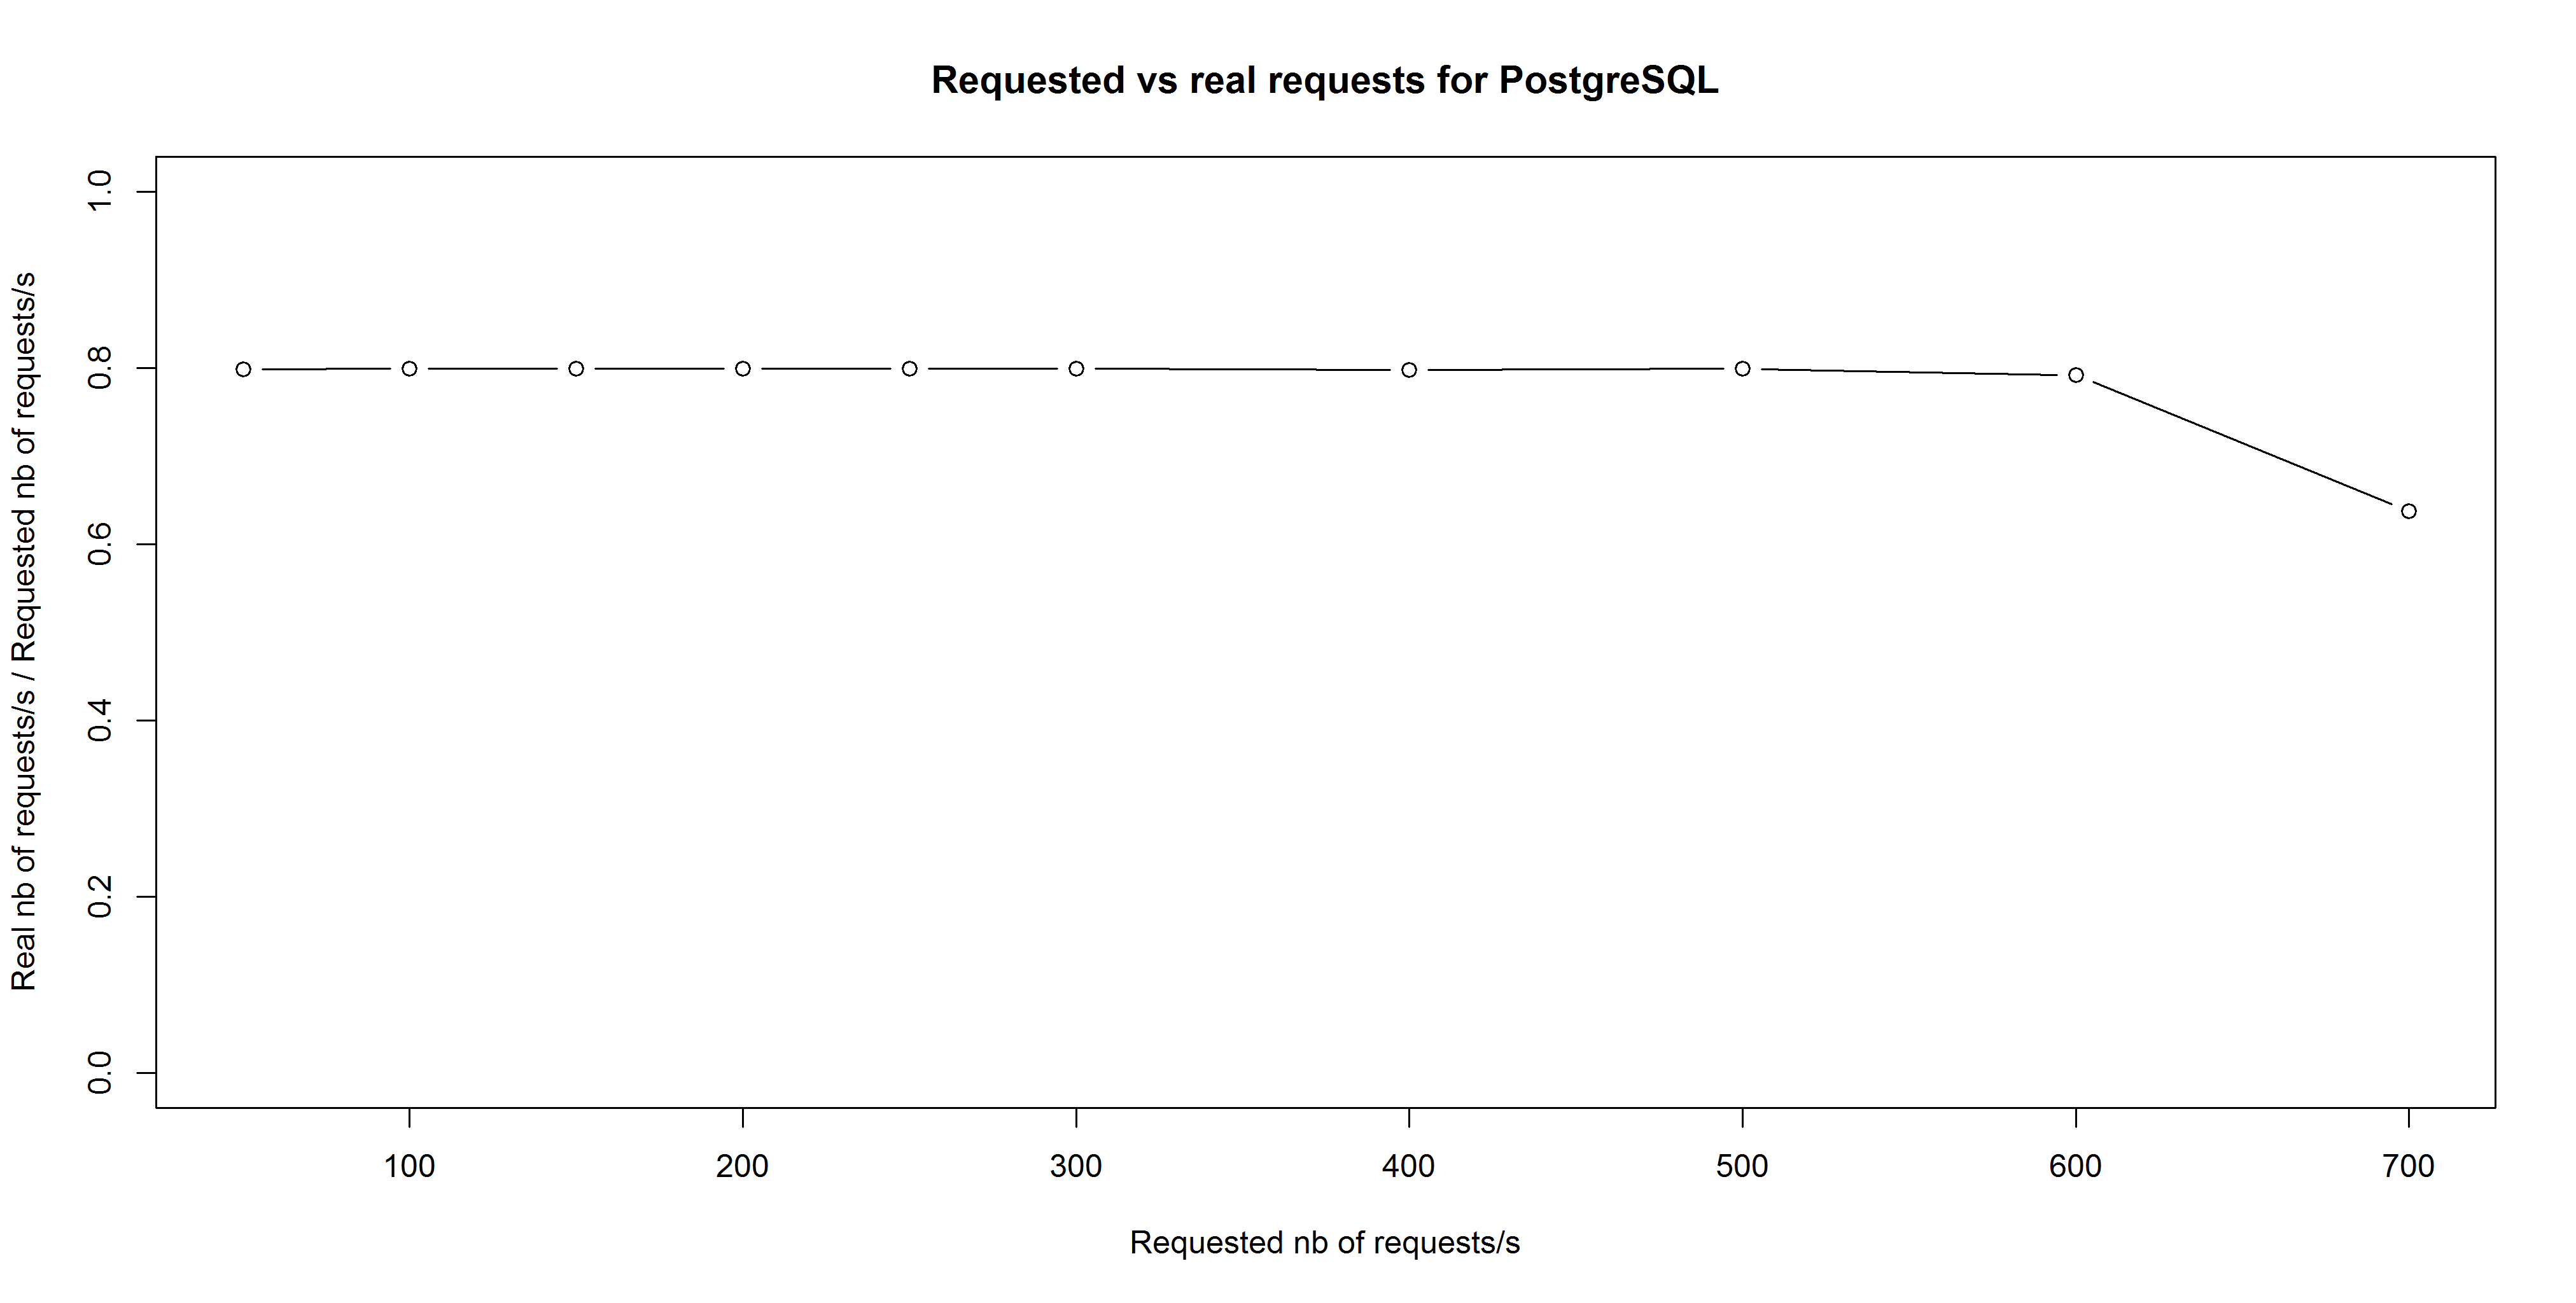
\includegraphics[width=\textwidth]{img/Observaties/loadbalance-realthroughput-db-PostgreSQL}}
	\caption{Calibratie: Overzicht van de vertraging t.o.v. het theoretisch aantal aanvragen met een vergelijking hoeveel werkelijke aanvragen er waren voor Pgpool-II. }
	\label{fig:calibratie-queriesperseconde-pgpool-ii}
\end{figure}

\section{Beschikbaarheidstest}
Bij de beschikbaarheidstesten kunnen de gegevens op verschillende manieren voorgesteld worden: de vertraging per query over de hele test, de vertraging tijdens het stoppen en starten van systemen of een vergelijking van de vertraging voor het stoppen (150-250s), na het herstarten (700-800s) en tussen het stoppen en starten(400-500s). 

Voor elk van de systemen is voor al de acties op de verschillende instanties data in voorhand, maar slechts enkele grafieken zullen getoond worden. Al de grafieken kunnen gevonden worden op GitHub op de link gegeven in het begin van het hoofdstuk. 

Een punt op de grafiek stelt de gemiddelde vertraging van 1 seconde voor, de lijn het gemiddelde over 10 seconden. 

\paragraph{HBase}
Bij HBase zijn er verschillende reacties op het stopzetten van een node. Bij het zacht stoppen van een instantie, is er een onderbreking van gemiddeld 20 seconde in de testen. Daarna kunnen er nog verhogingen in de queries af en toe optreden. Zie figuur \ref{fig:beschikbaar-hbase-soft}. 

Bij de netwerk onderbreking is er in de testen een onderbreking van ongeveer 100 seconden. Daarna is het terug stabiel. Zie figuur \ref{fig:beschikbaar-hbase-drop}

Bij een harde stop is er een combinatie van de netwerk onderbreking én is het af en toe zo dat de volledige periode geen queries mogelijk zijn. Zie figuur \ref{fig:beschikbaar-hbase-drop} en \ref{fig:beschikbaar-hbase-hard}

Tijdens de onderbreking, is er geen significante verandering in de vertraging van de uitgevoerde queries gemeten. 
\begin{figure}[ht!] 
	\centering
	\subfigure[Voorbeeld zacht stop]{\label{fig:beschikbaar-hbase-soft} 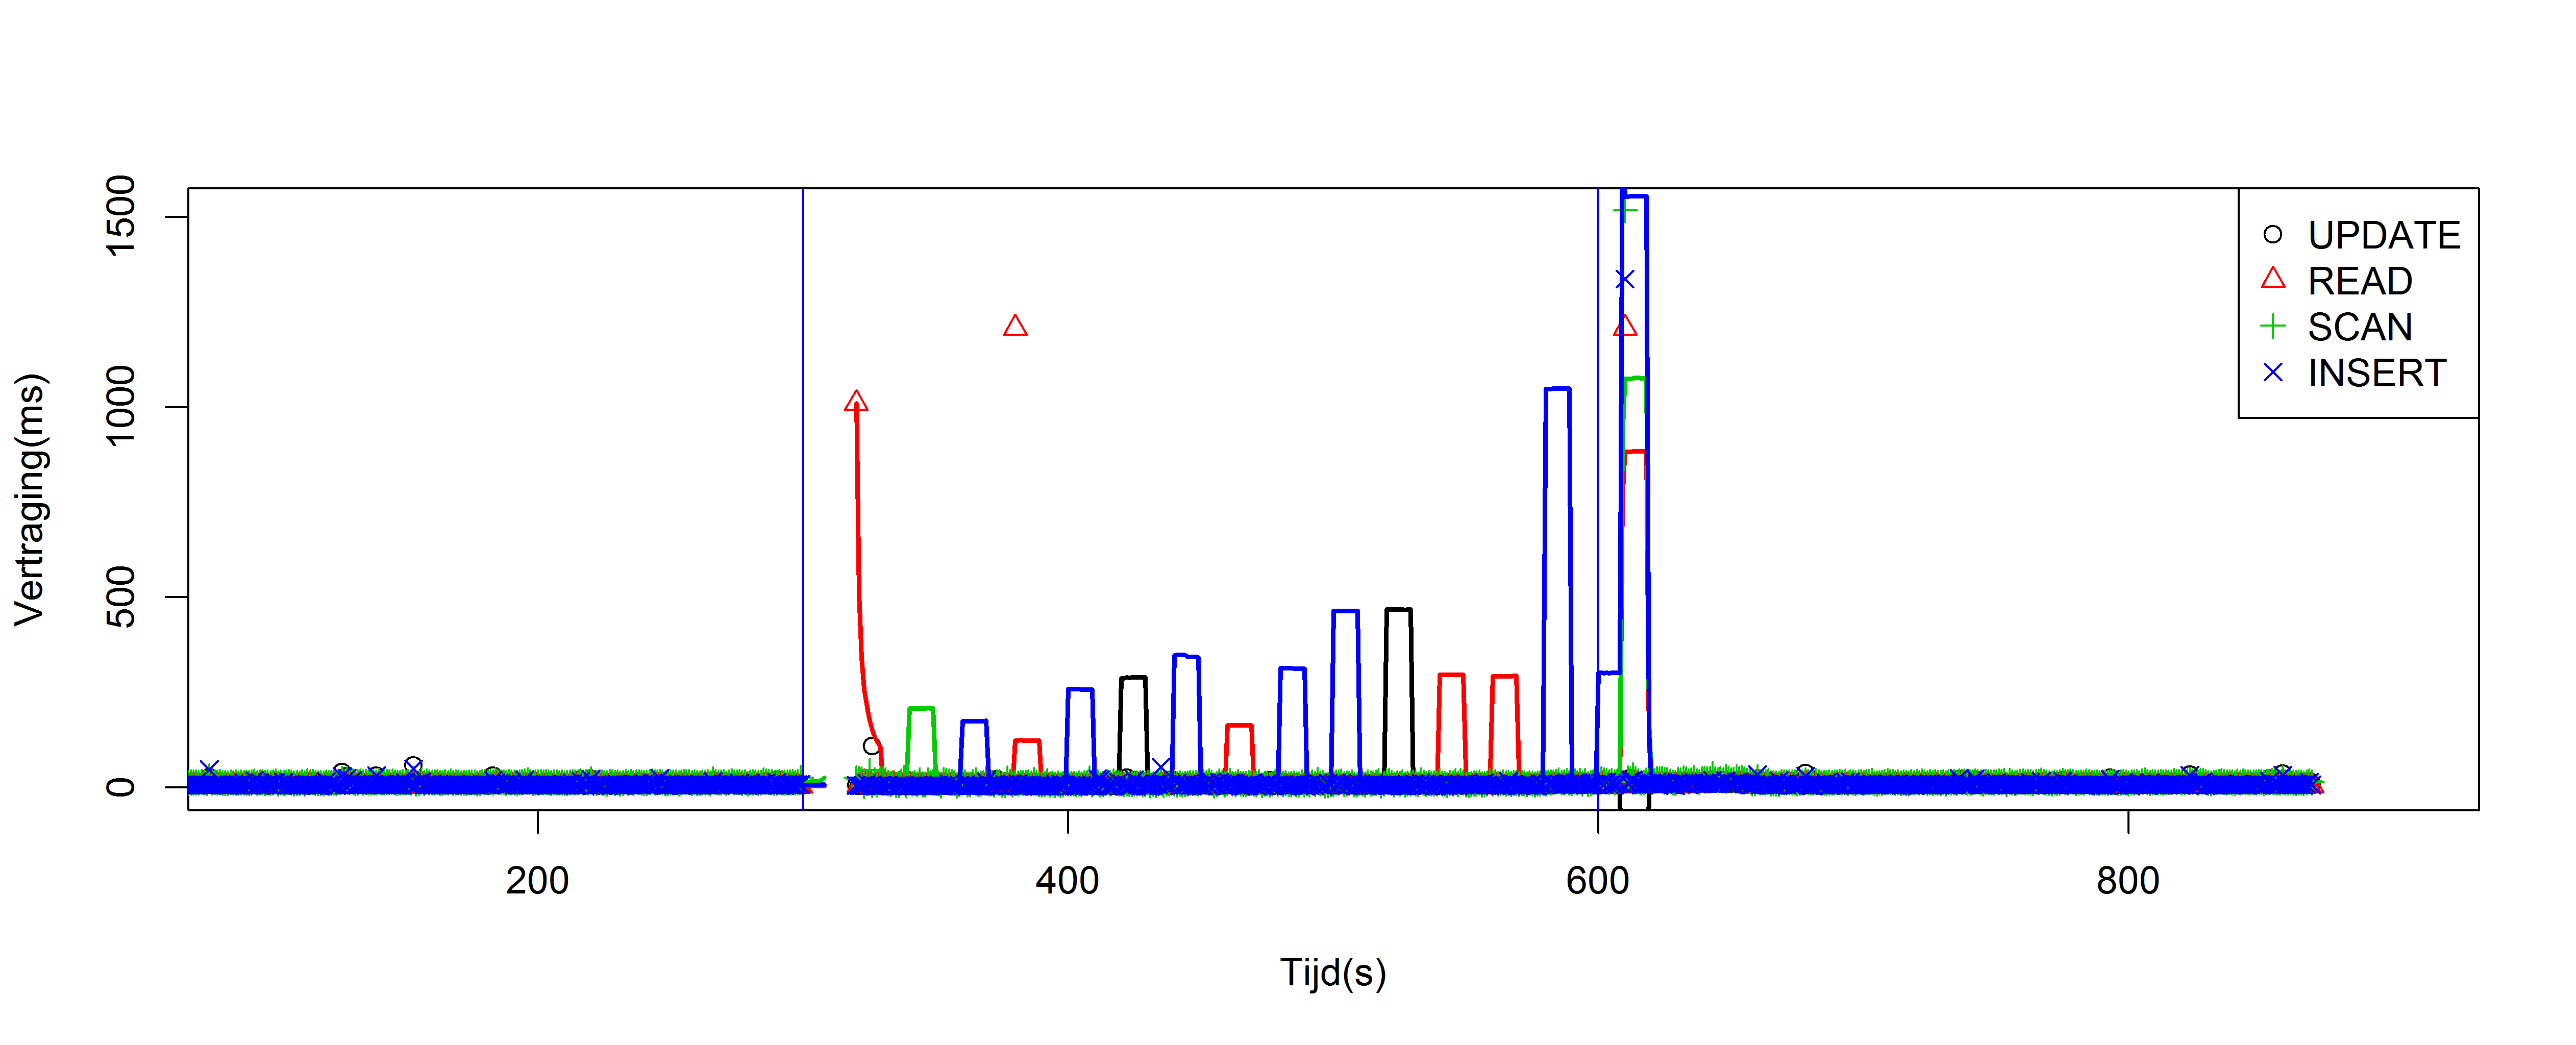
\includegraphics[width=\textwidth]{img/Observaties/HBase/single-graph-2-1}}
	\subfigure[Voorbeeld netwerk onderbreking en harde stop]{\label{fig:beschikbaar-hbase-drop} 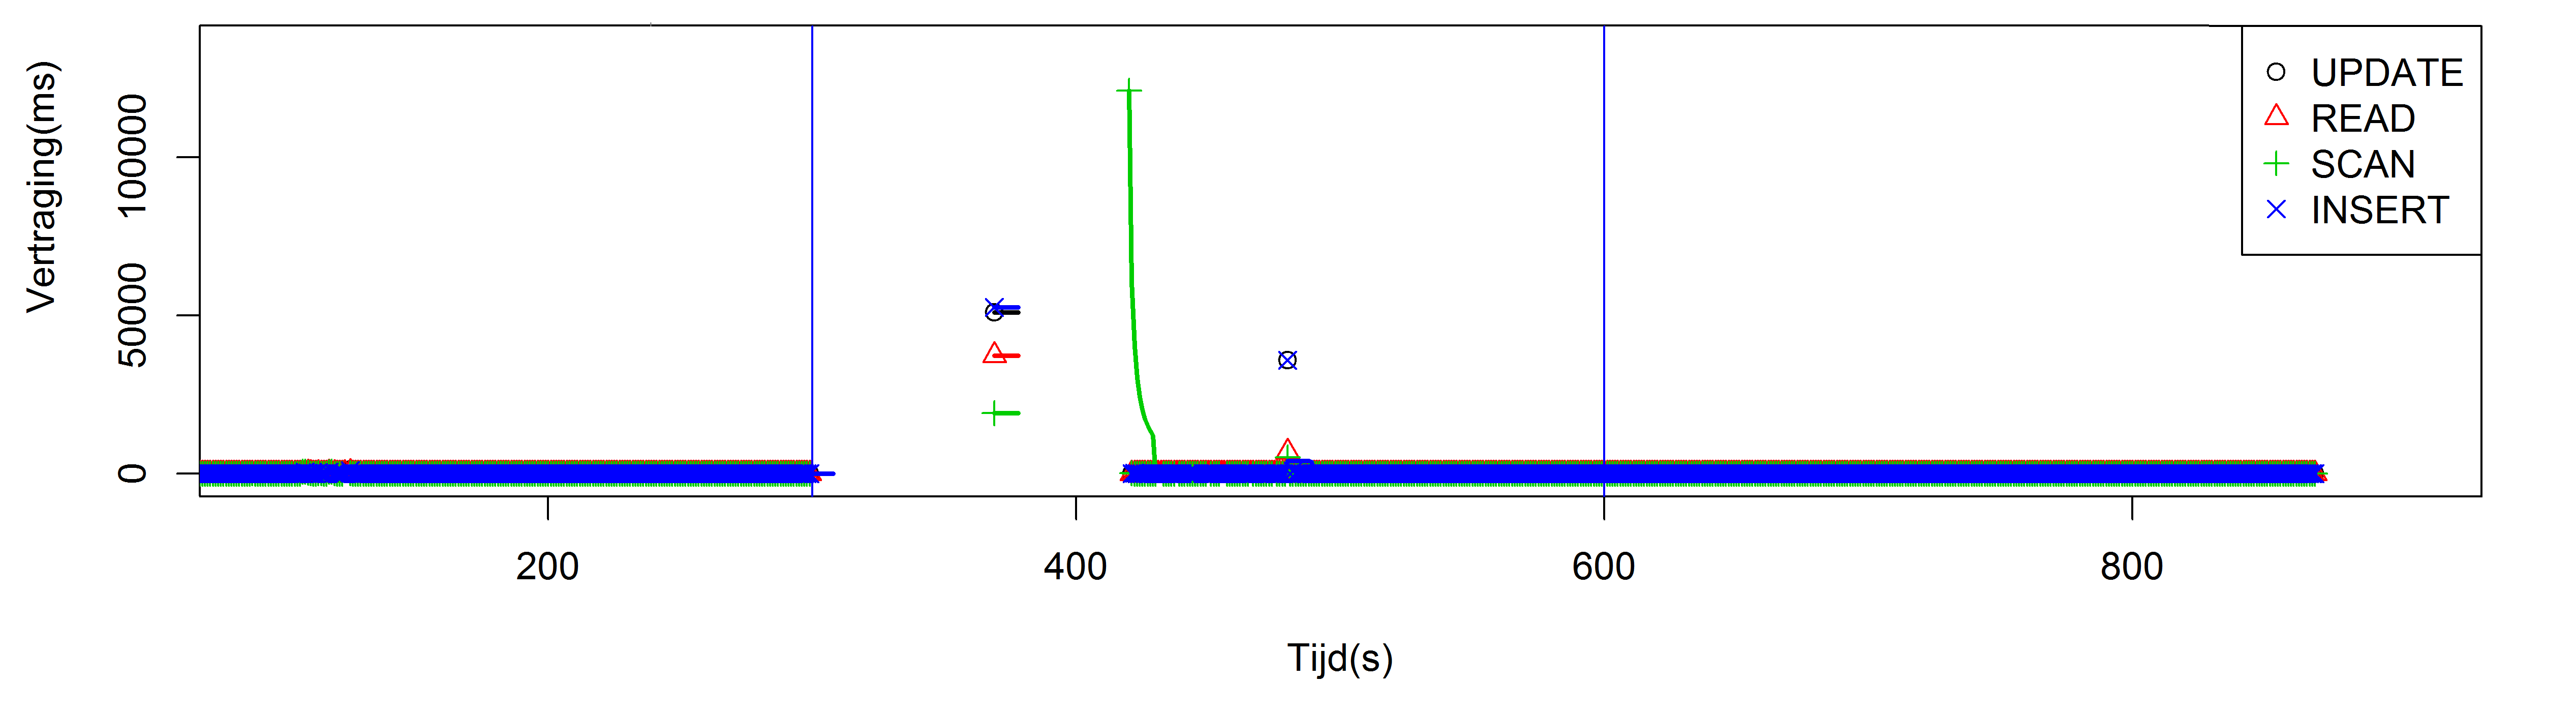
\includegraphics[width=\textwidth]{img/Observaties/HBase/single-graph-2-drop-1}}
	\subfigure[Voorbeeld hard stop]{\label{fig:beschikbaar-hbase-hard} 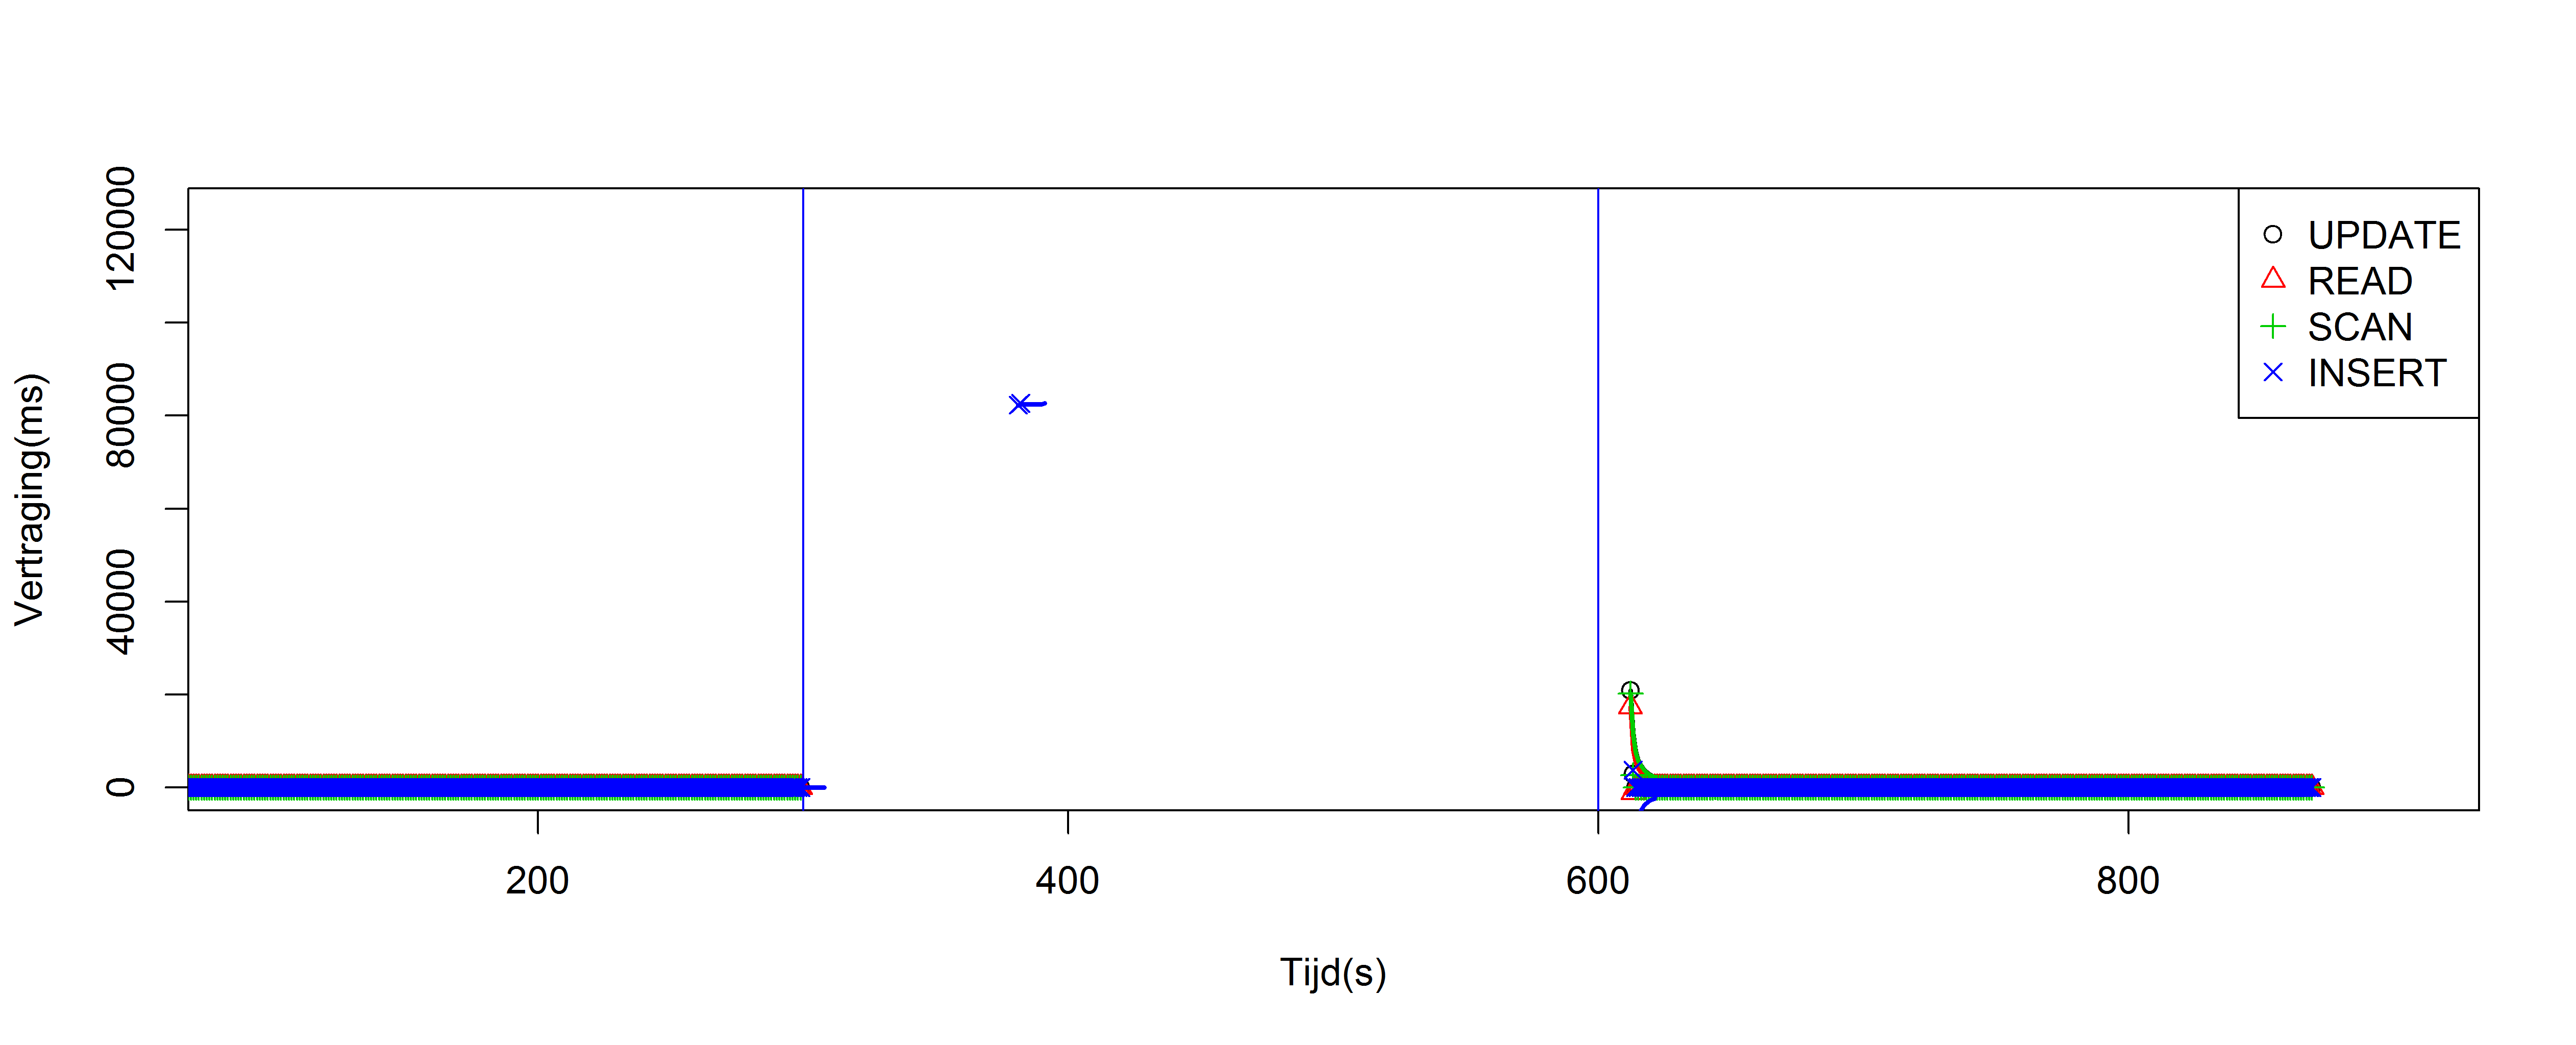
\includegraphics[width=\textwidth]{img/Observaties/HBase/single-graph-3-kill-1}}
	\caption{Beschikbaarheid: Verschillende voorbeeldreacties van HBase op beschikbaarheidstesten }
	\label{fig:beschikbaar-hbase-1}
\end{figure}

\paragraph{MongoDB} \todo{}
Ook bij MongoDB zijn er verschillende reacties op het stopzetten als men de queries onder standaard configuratie uitvoert. In het geval van zacht of hard stoppen is er geen verschil in de reactie, bij 2/3 van de keren is er geen verschil merkbaar, bij 1/3 van de keren is er tijdelijke verhoging van het aantal queries, een voorbeeld toont dat de scan operatie voor 2 seconden uitgesteld wordt. Figuur van het overzicht: \ref{fig:beschikbaar-mongodb-soft} met een zoom naar de stop \ref{fig:beschikbaar-mongodb-soft-zoom}.

Bij het onderbreken van het netwerk is er in bepaalde geen significante verandering, op andere momenten is een gedrag soortgelijk aan dat bij een zachte stop te merken. In andere gevallen is het zo dat er geen queries mogelijk zijn gedurende de volledige netwerk onderbreking. Zie figuur \ref{fig:beschikbaar-mongodb-drop}. 

Tijdens de onderbreking, is er geen significante verandering in de vertraging van de uitgevoerde queries gemeten. 
\begin{figure}[ht!] 
	\centering
	\subfigure[Voorbeeld van een zacht stop, harde stop en netwerk onderbreking]{\label{fig:beschikbaar-mongodb-soft} 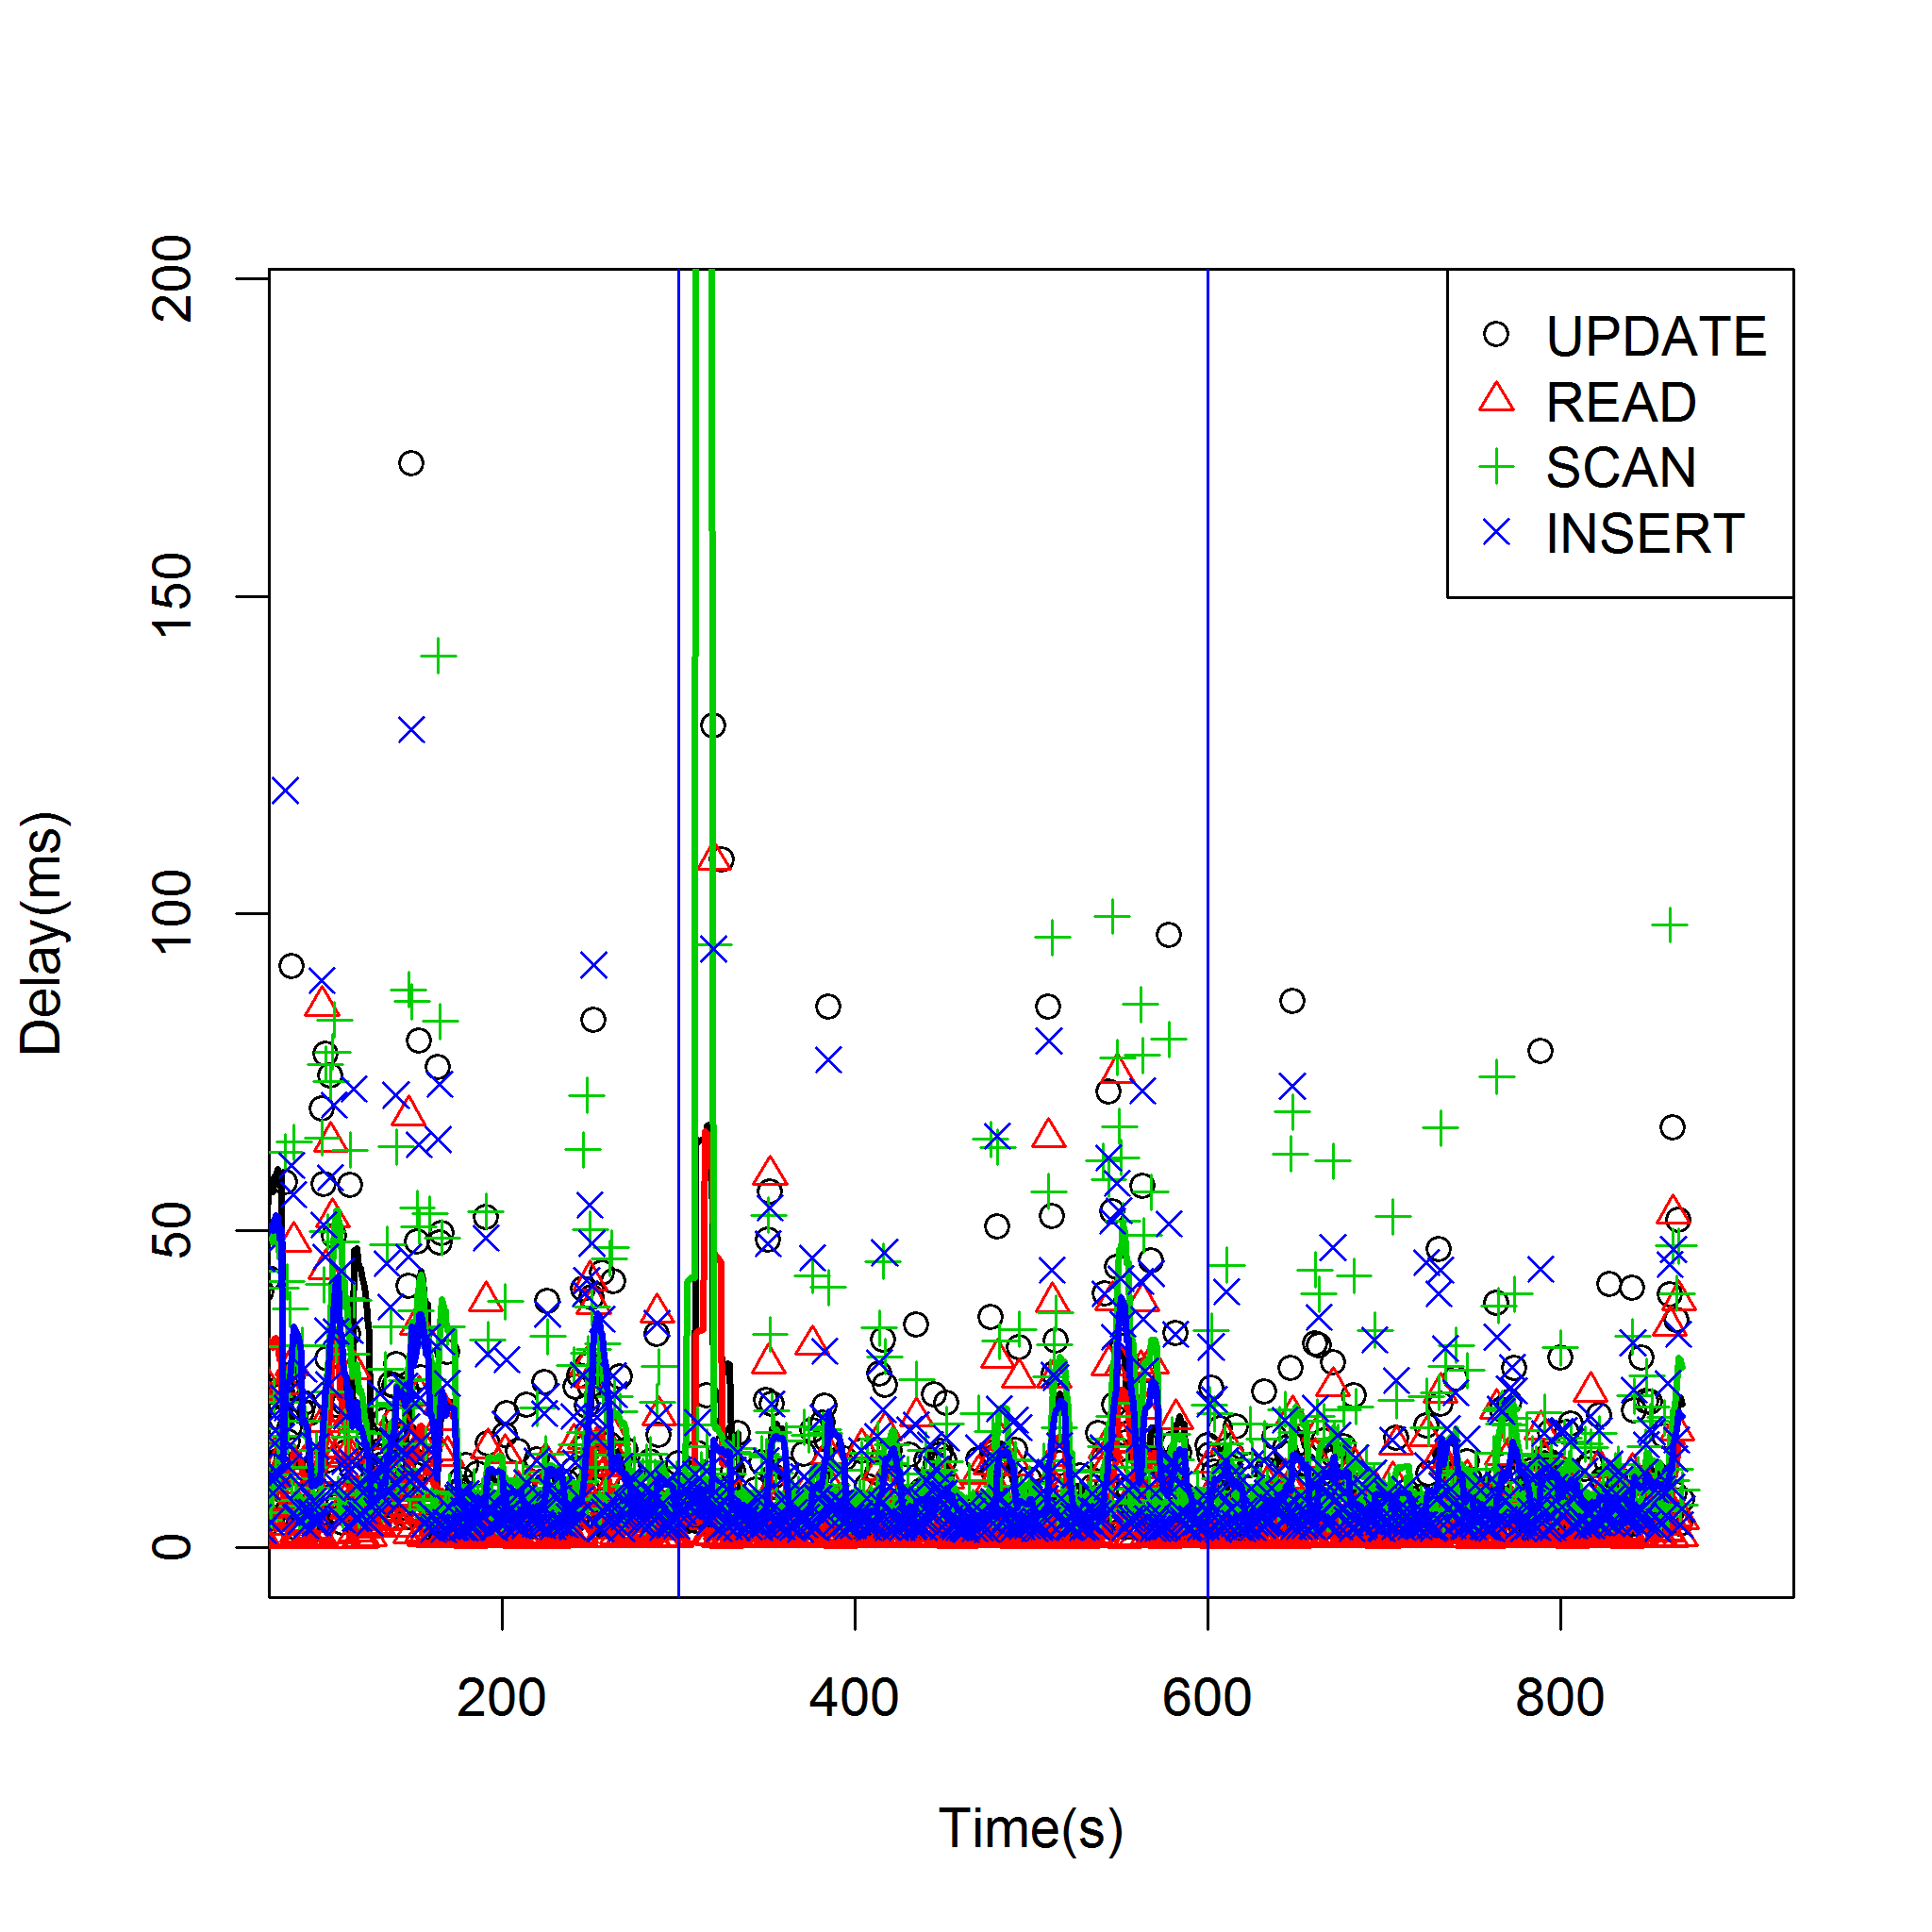
\includegraphics[width=\textwidth]{img/Observaties/MongoDB/single-graph-6-1}}
	\subfigure[Zacht stop met inzoomen op het uitschakelen]{\label{fig:beschikbaar-mongodb-soft-zoom} 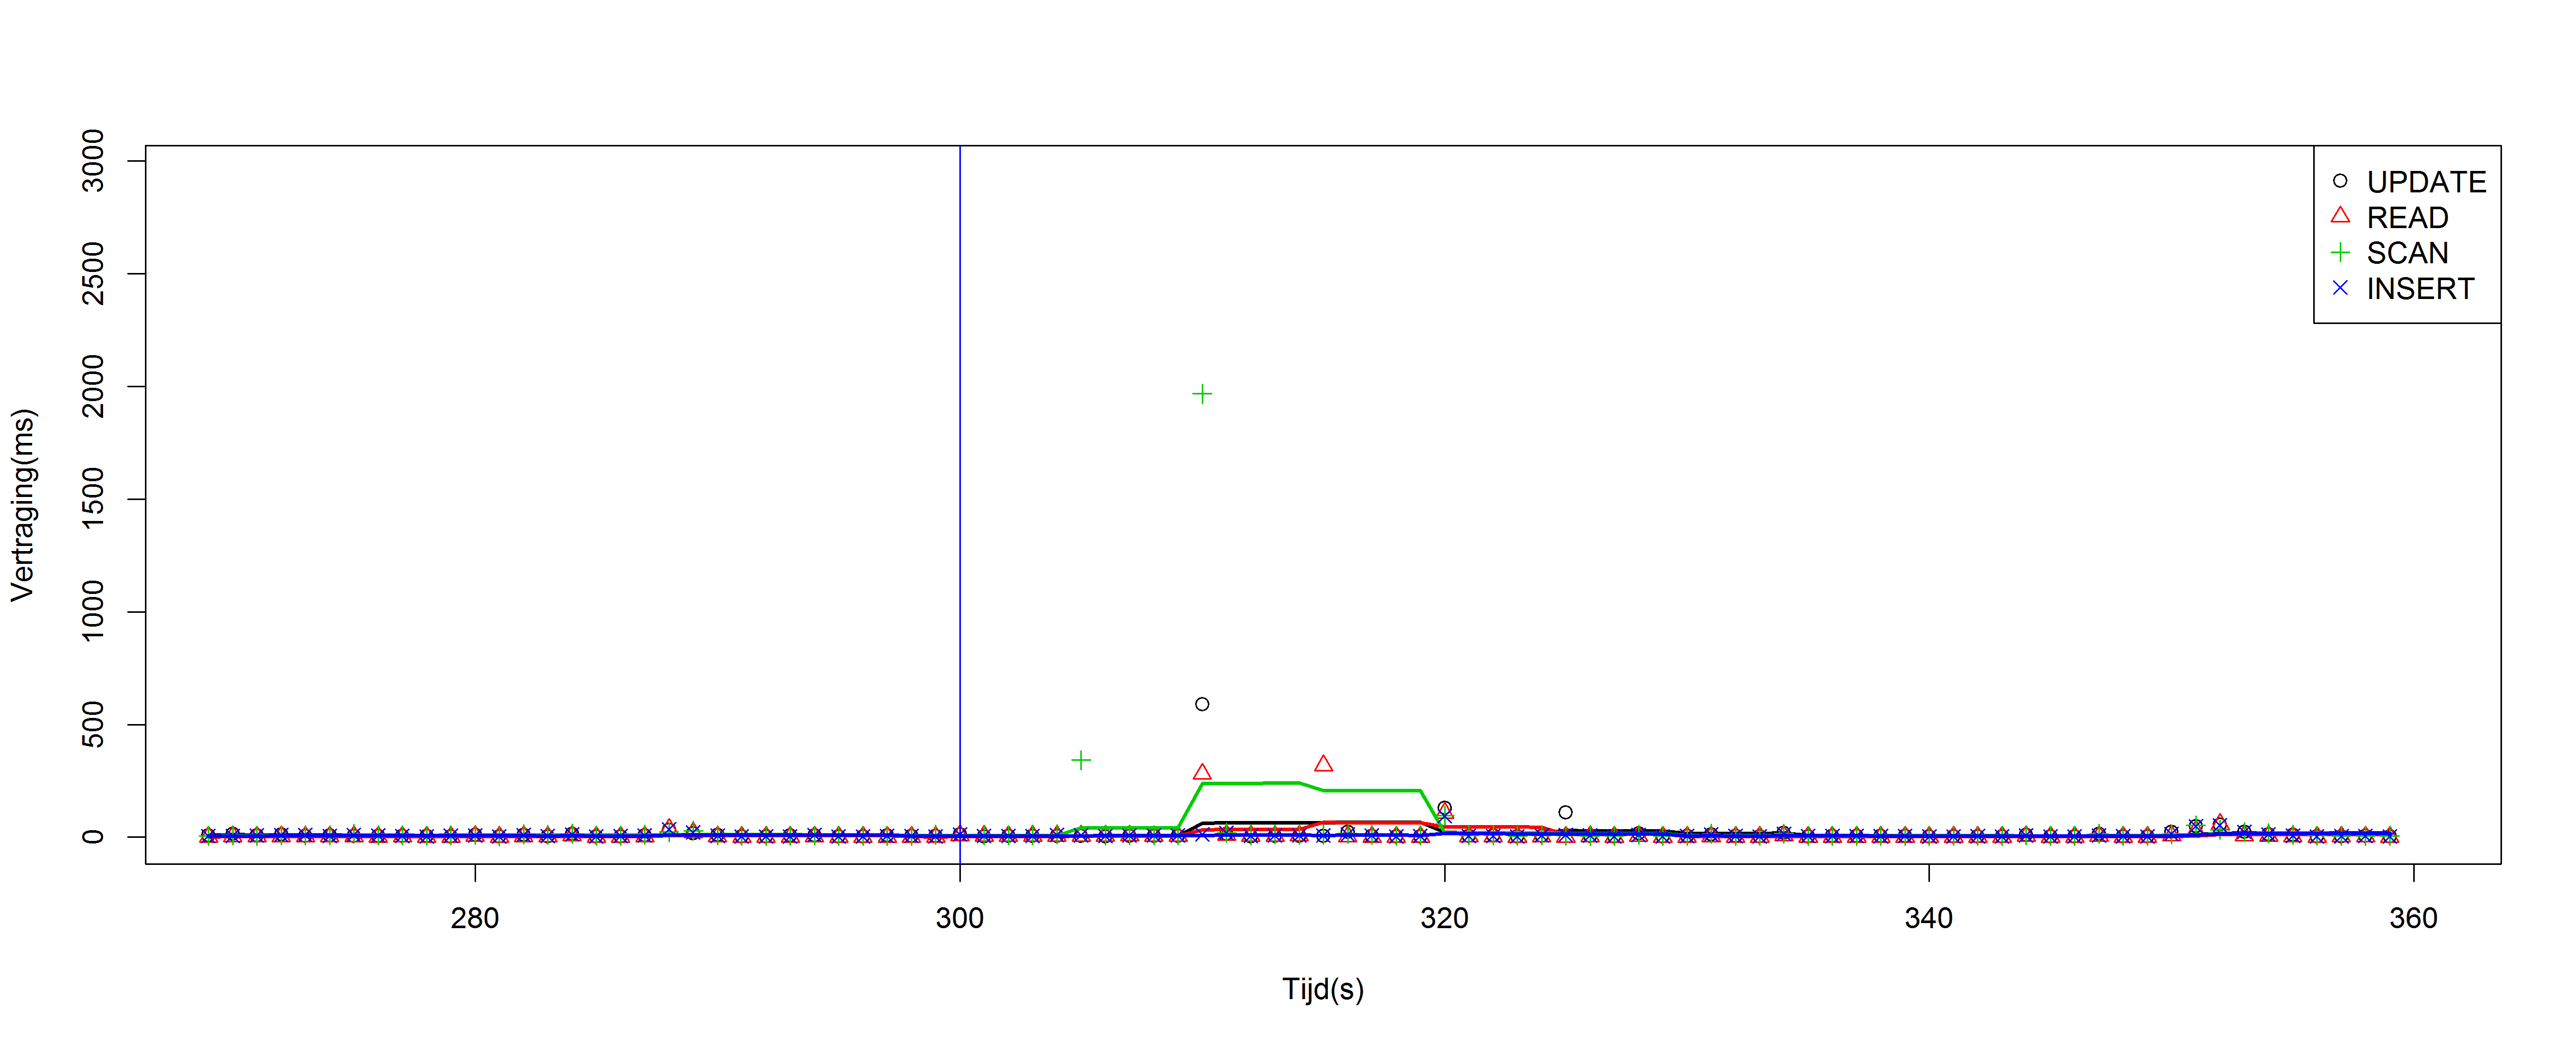
\includegraphics[width=\textwidth]{img/Observaties/MongoDB/multiple-graph-interrupt-Node-6-Shut-down}}
	\subfigure[Voorbeeld netwerk onderbreking ]{\label{fig:beschikbaar-mongodb-drop} 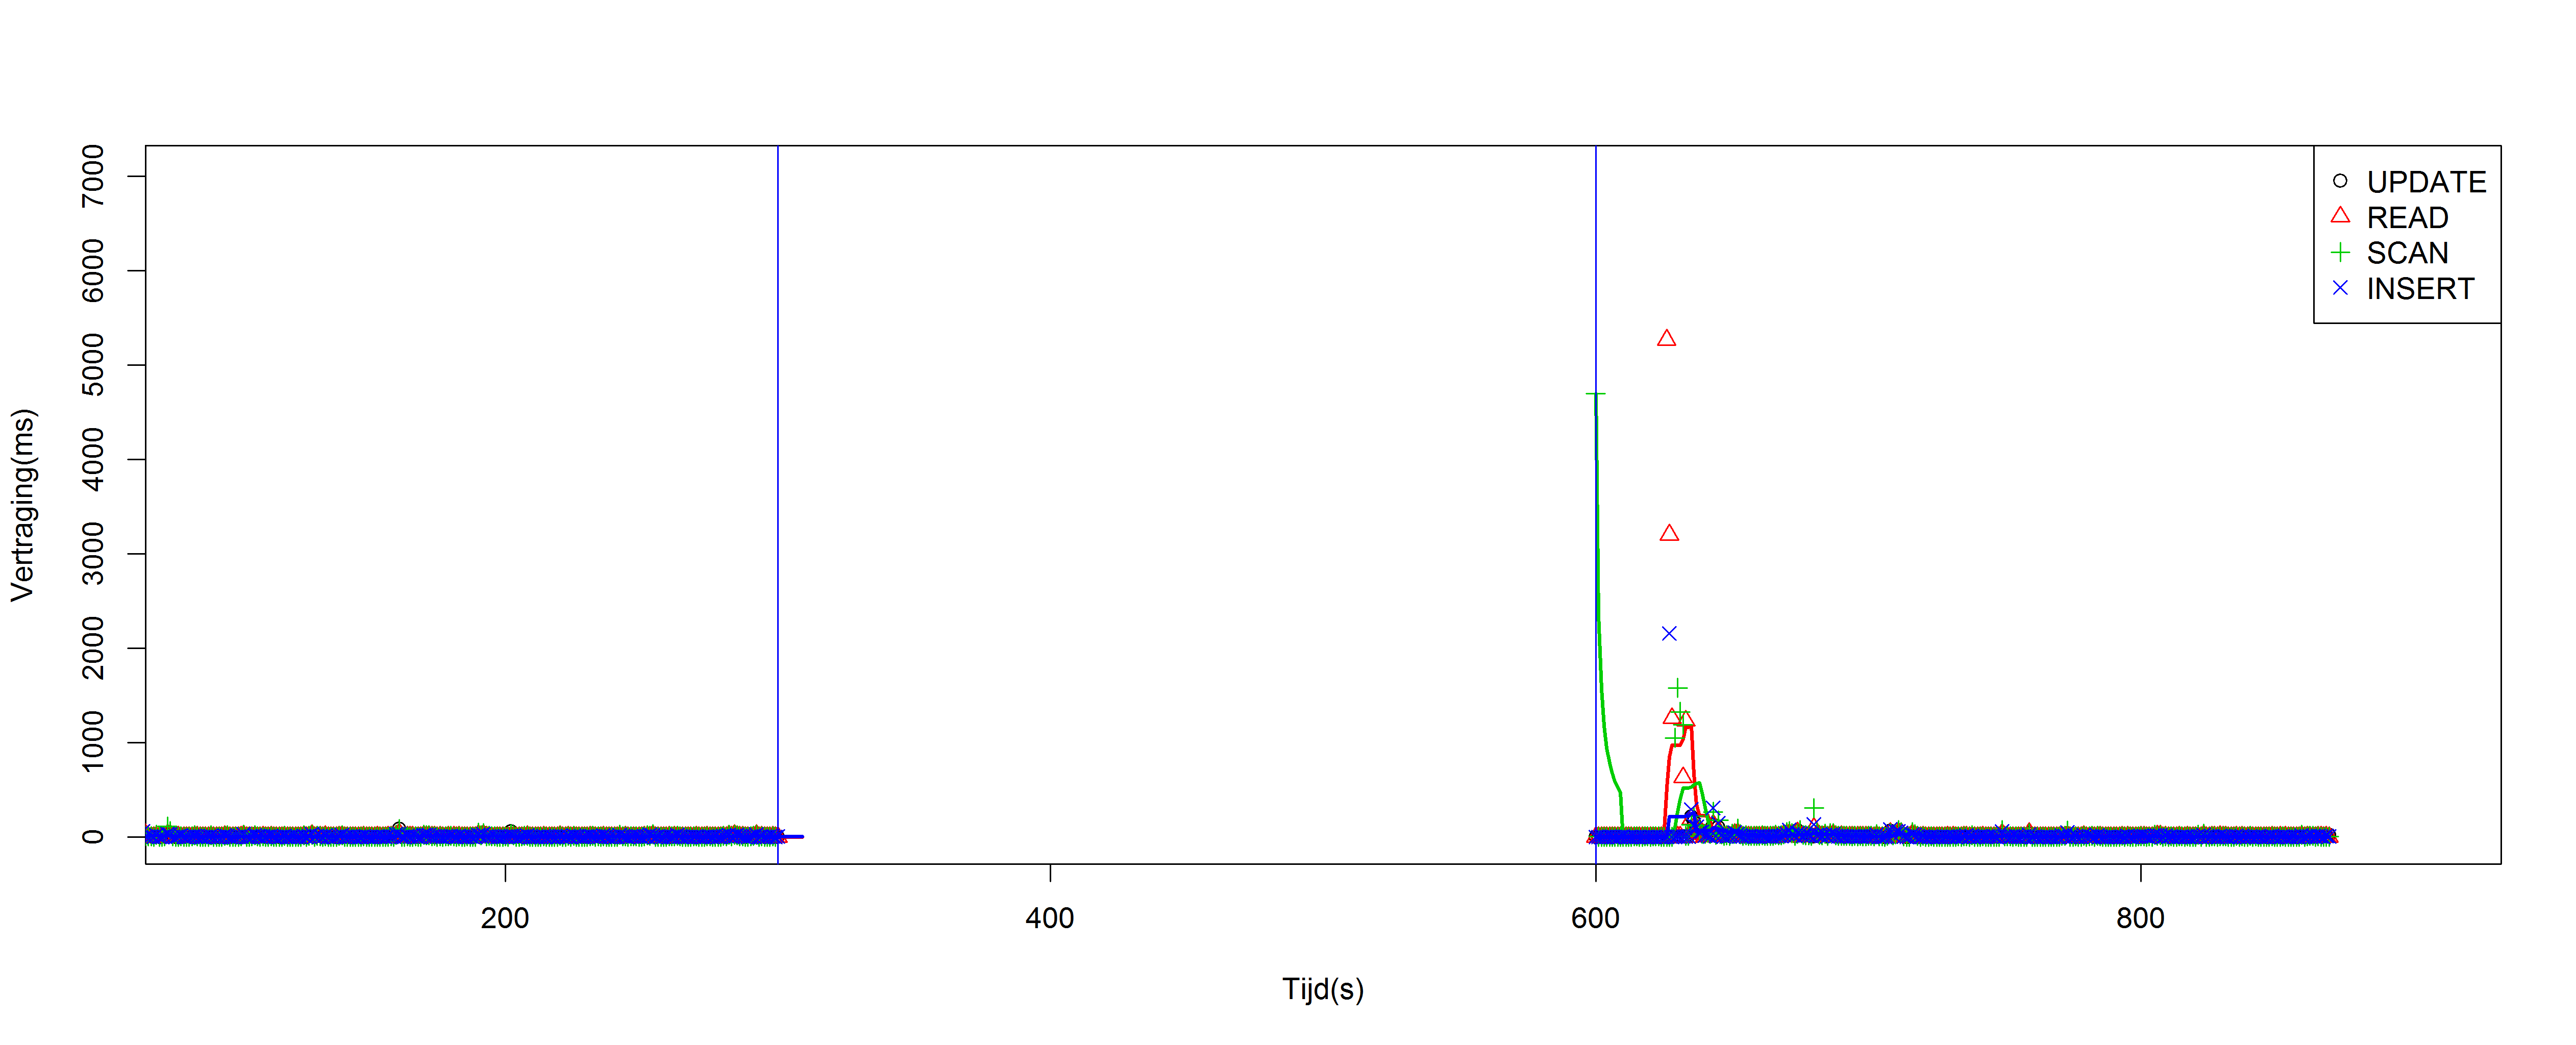
\includegraphics[width=\textwidth]{img/Observaties/MongoDB/single-graph-4-drop-1}}
	\caption{Beschikbaarheid: Verschillende voorbeeldreacties van MongoDB op beschikbaarheidstesten }
	\label{fig:beschikbaar-mongodb-1}
\end{figure}

\paragraph{Pgpool-II} Bij Pgpool-II is een gr\todo{}

In het geval van een zachte stop, is er tijdelijk een onderbreking van al de queries, de queries worden tijdelijk vertraagd met ongeveer 2 seconden, een voorbeeld bevindt zich in figuur \ref{fig:beschikbaar-pgpool-soft}. 

Bij een netwerk onderbreking, zijn er enige tijd geen queries mogelijk en na 30 seconden was de onderbreking over in de testen.  Een voorbeeld bevindt zich in figuur \ref{fig:beschikbaar-pgpool-netwerk}.  

Tijdens de onderbreking is er een verandering naar schrijf queries toe, deze nemen significant minder tijd in beslag, dit geldt niet voor lees queries. Het voorbeelden uit de testen bevinden zich in figuur \ref{fig:beschikbaar-pgpool-boxplot-read} en \ref{fig:beschikbaar-pgpool-boxplot-write} voor respectievelijk schrijf en lees queries. 
\begin{figure}[ht!] 
	\centering
	\subfigure[Voorbeeld van een zacht stop]{\label{fig:beschikbaar-pgpool-soft} 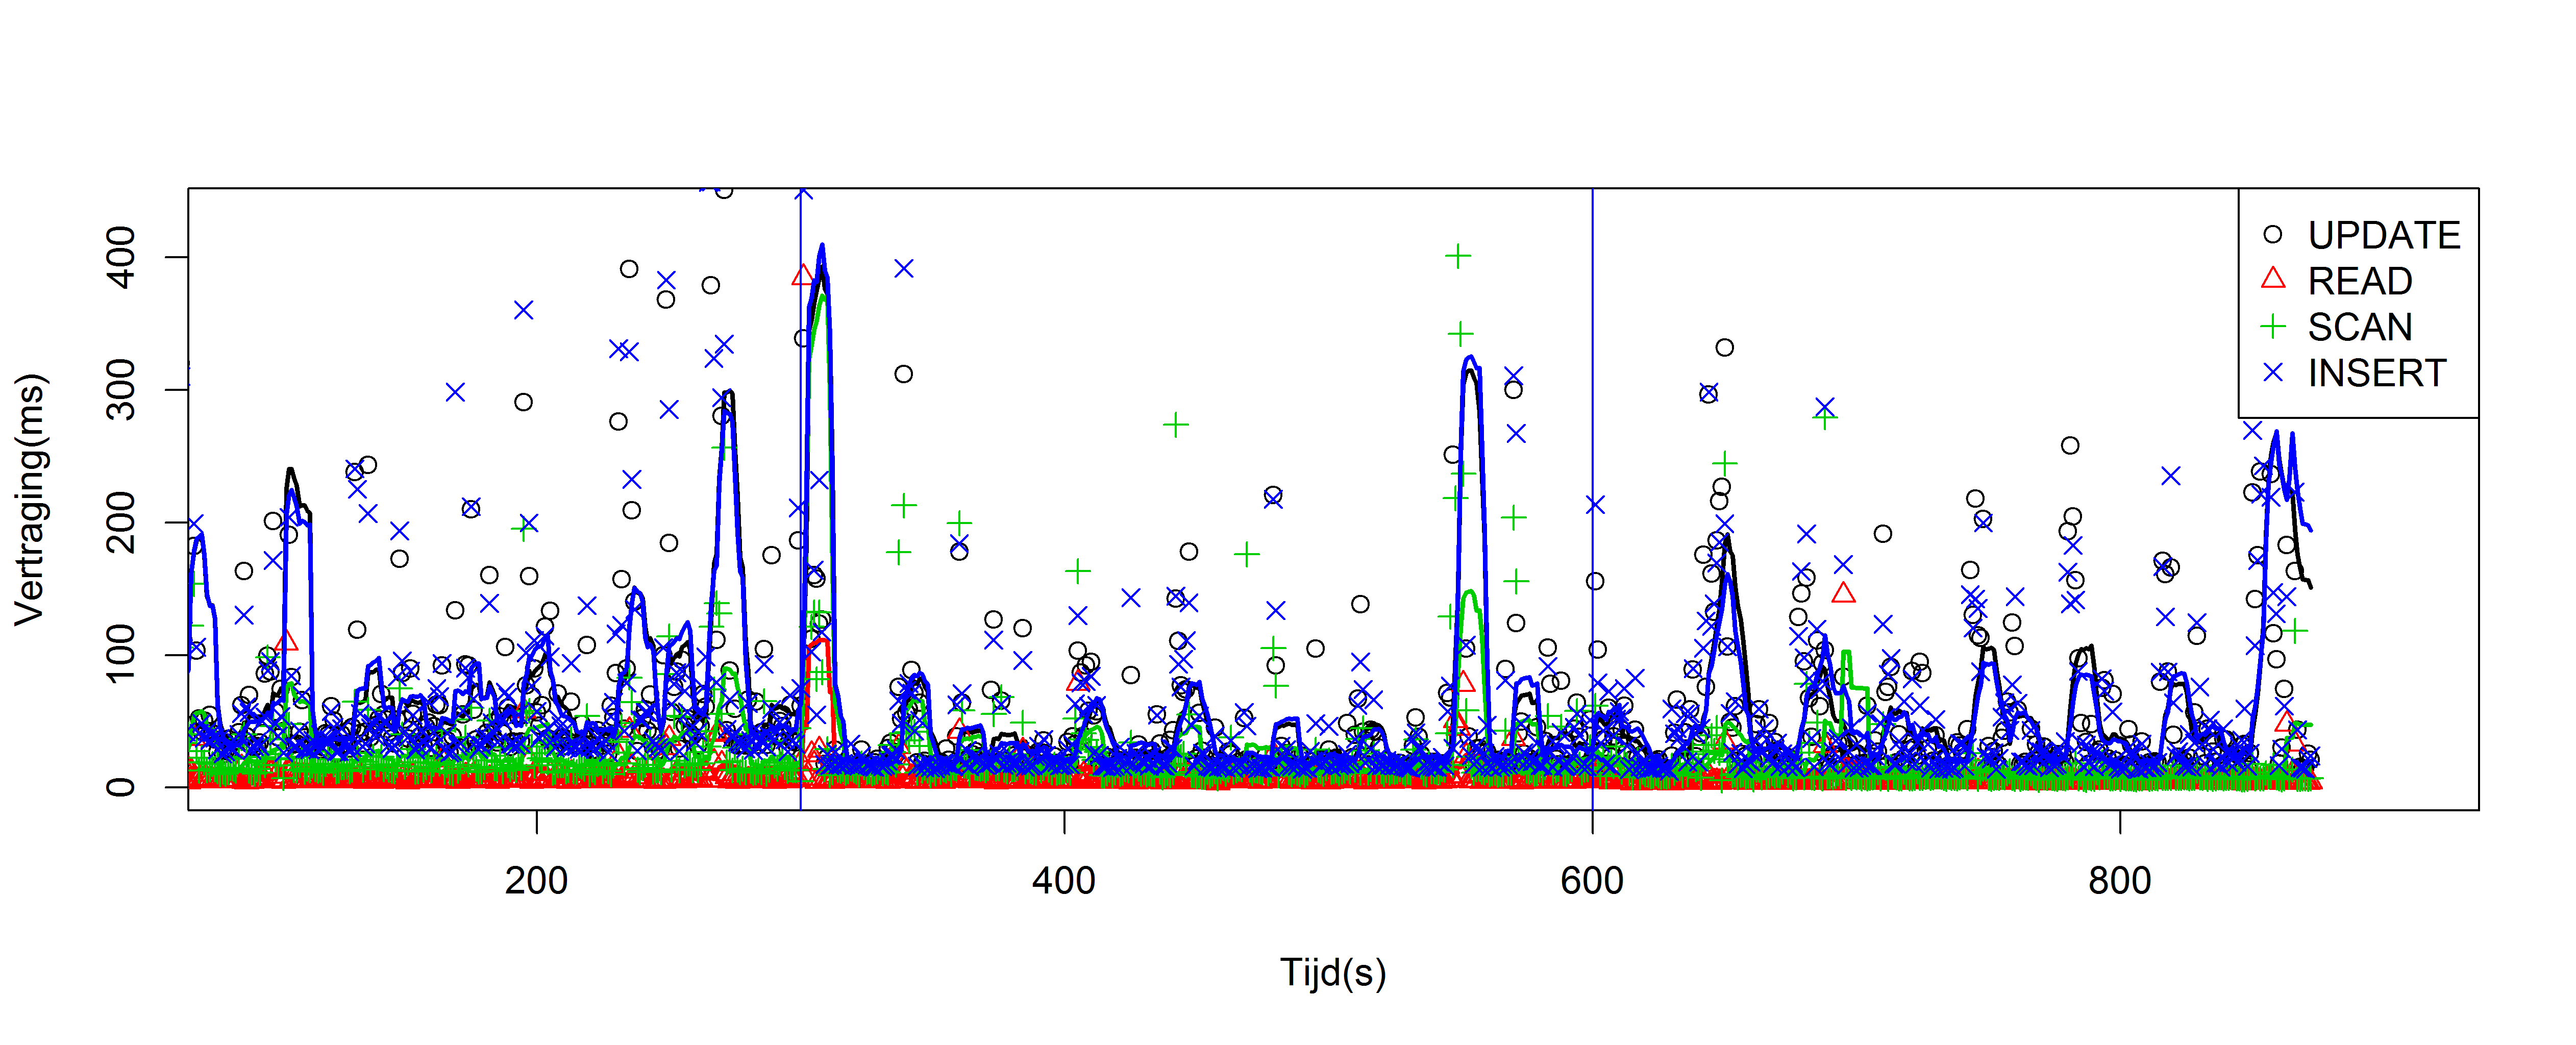
\includegraphics[width=\textwidth]{img/Observaties/Pgpool/single-graph-1-2}}
	\subfigure[Voorbeeld van een harde stop of netwerk onderbreking]{\label{fig:beschikbaar-pgpool-netwerk} 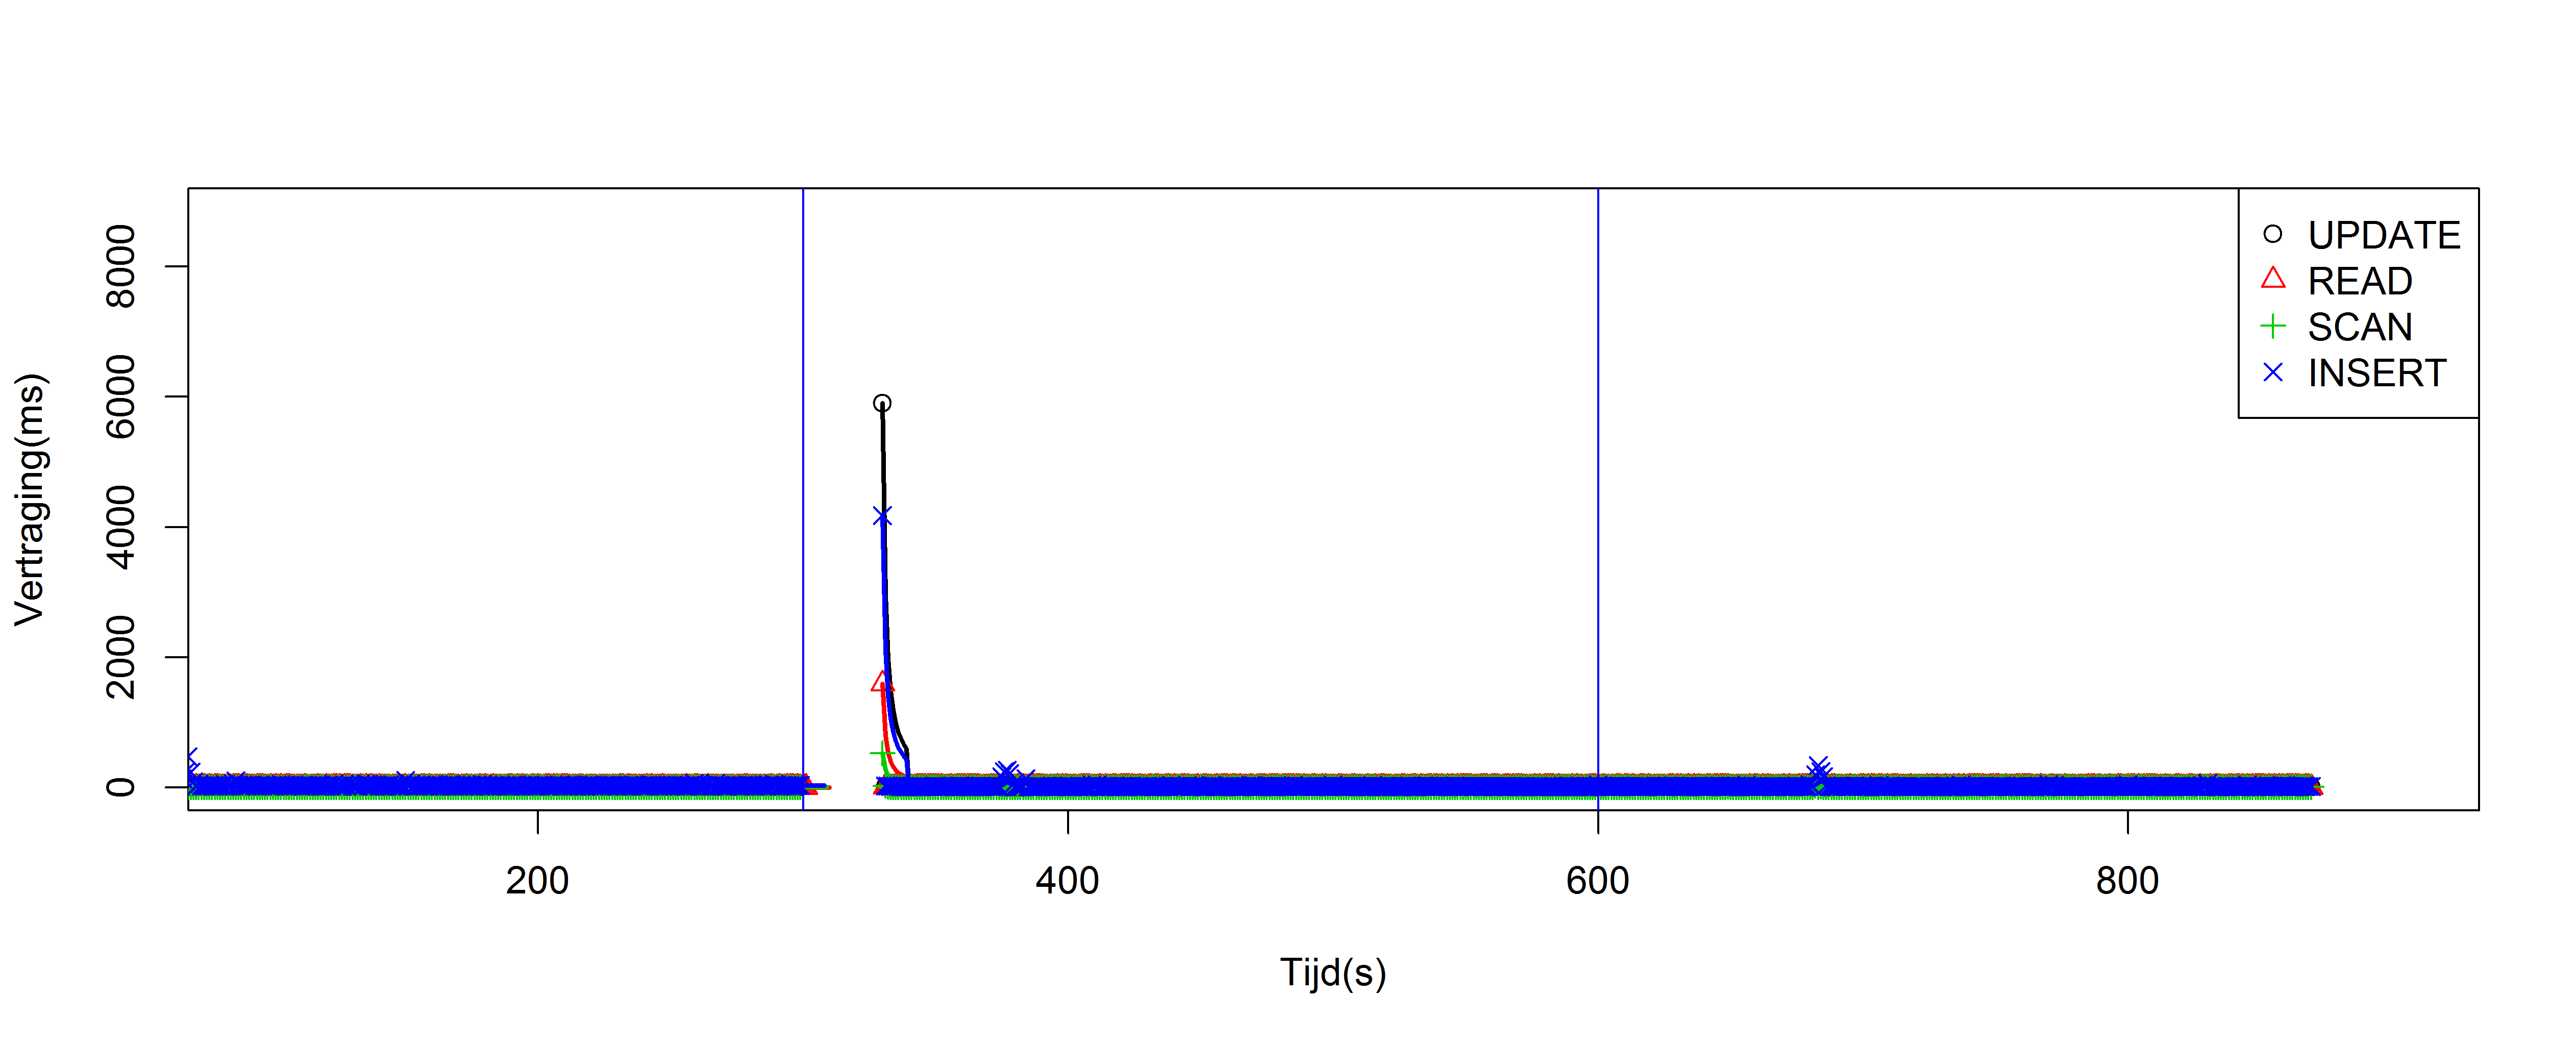
\includegraphics[width=\textwidth]{img/Observaties/Pgpool/single-graph-1-drop-1}}
	\subfigure[Boxplot met leesvertragingen]{\label{fig:beschikbaar-pgpool-boxplot-read} 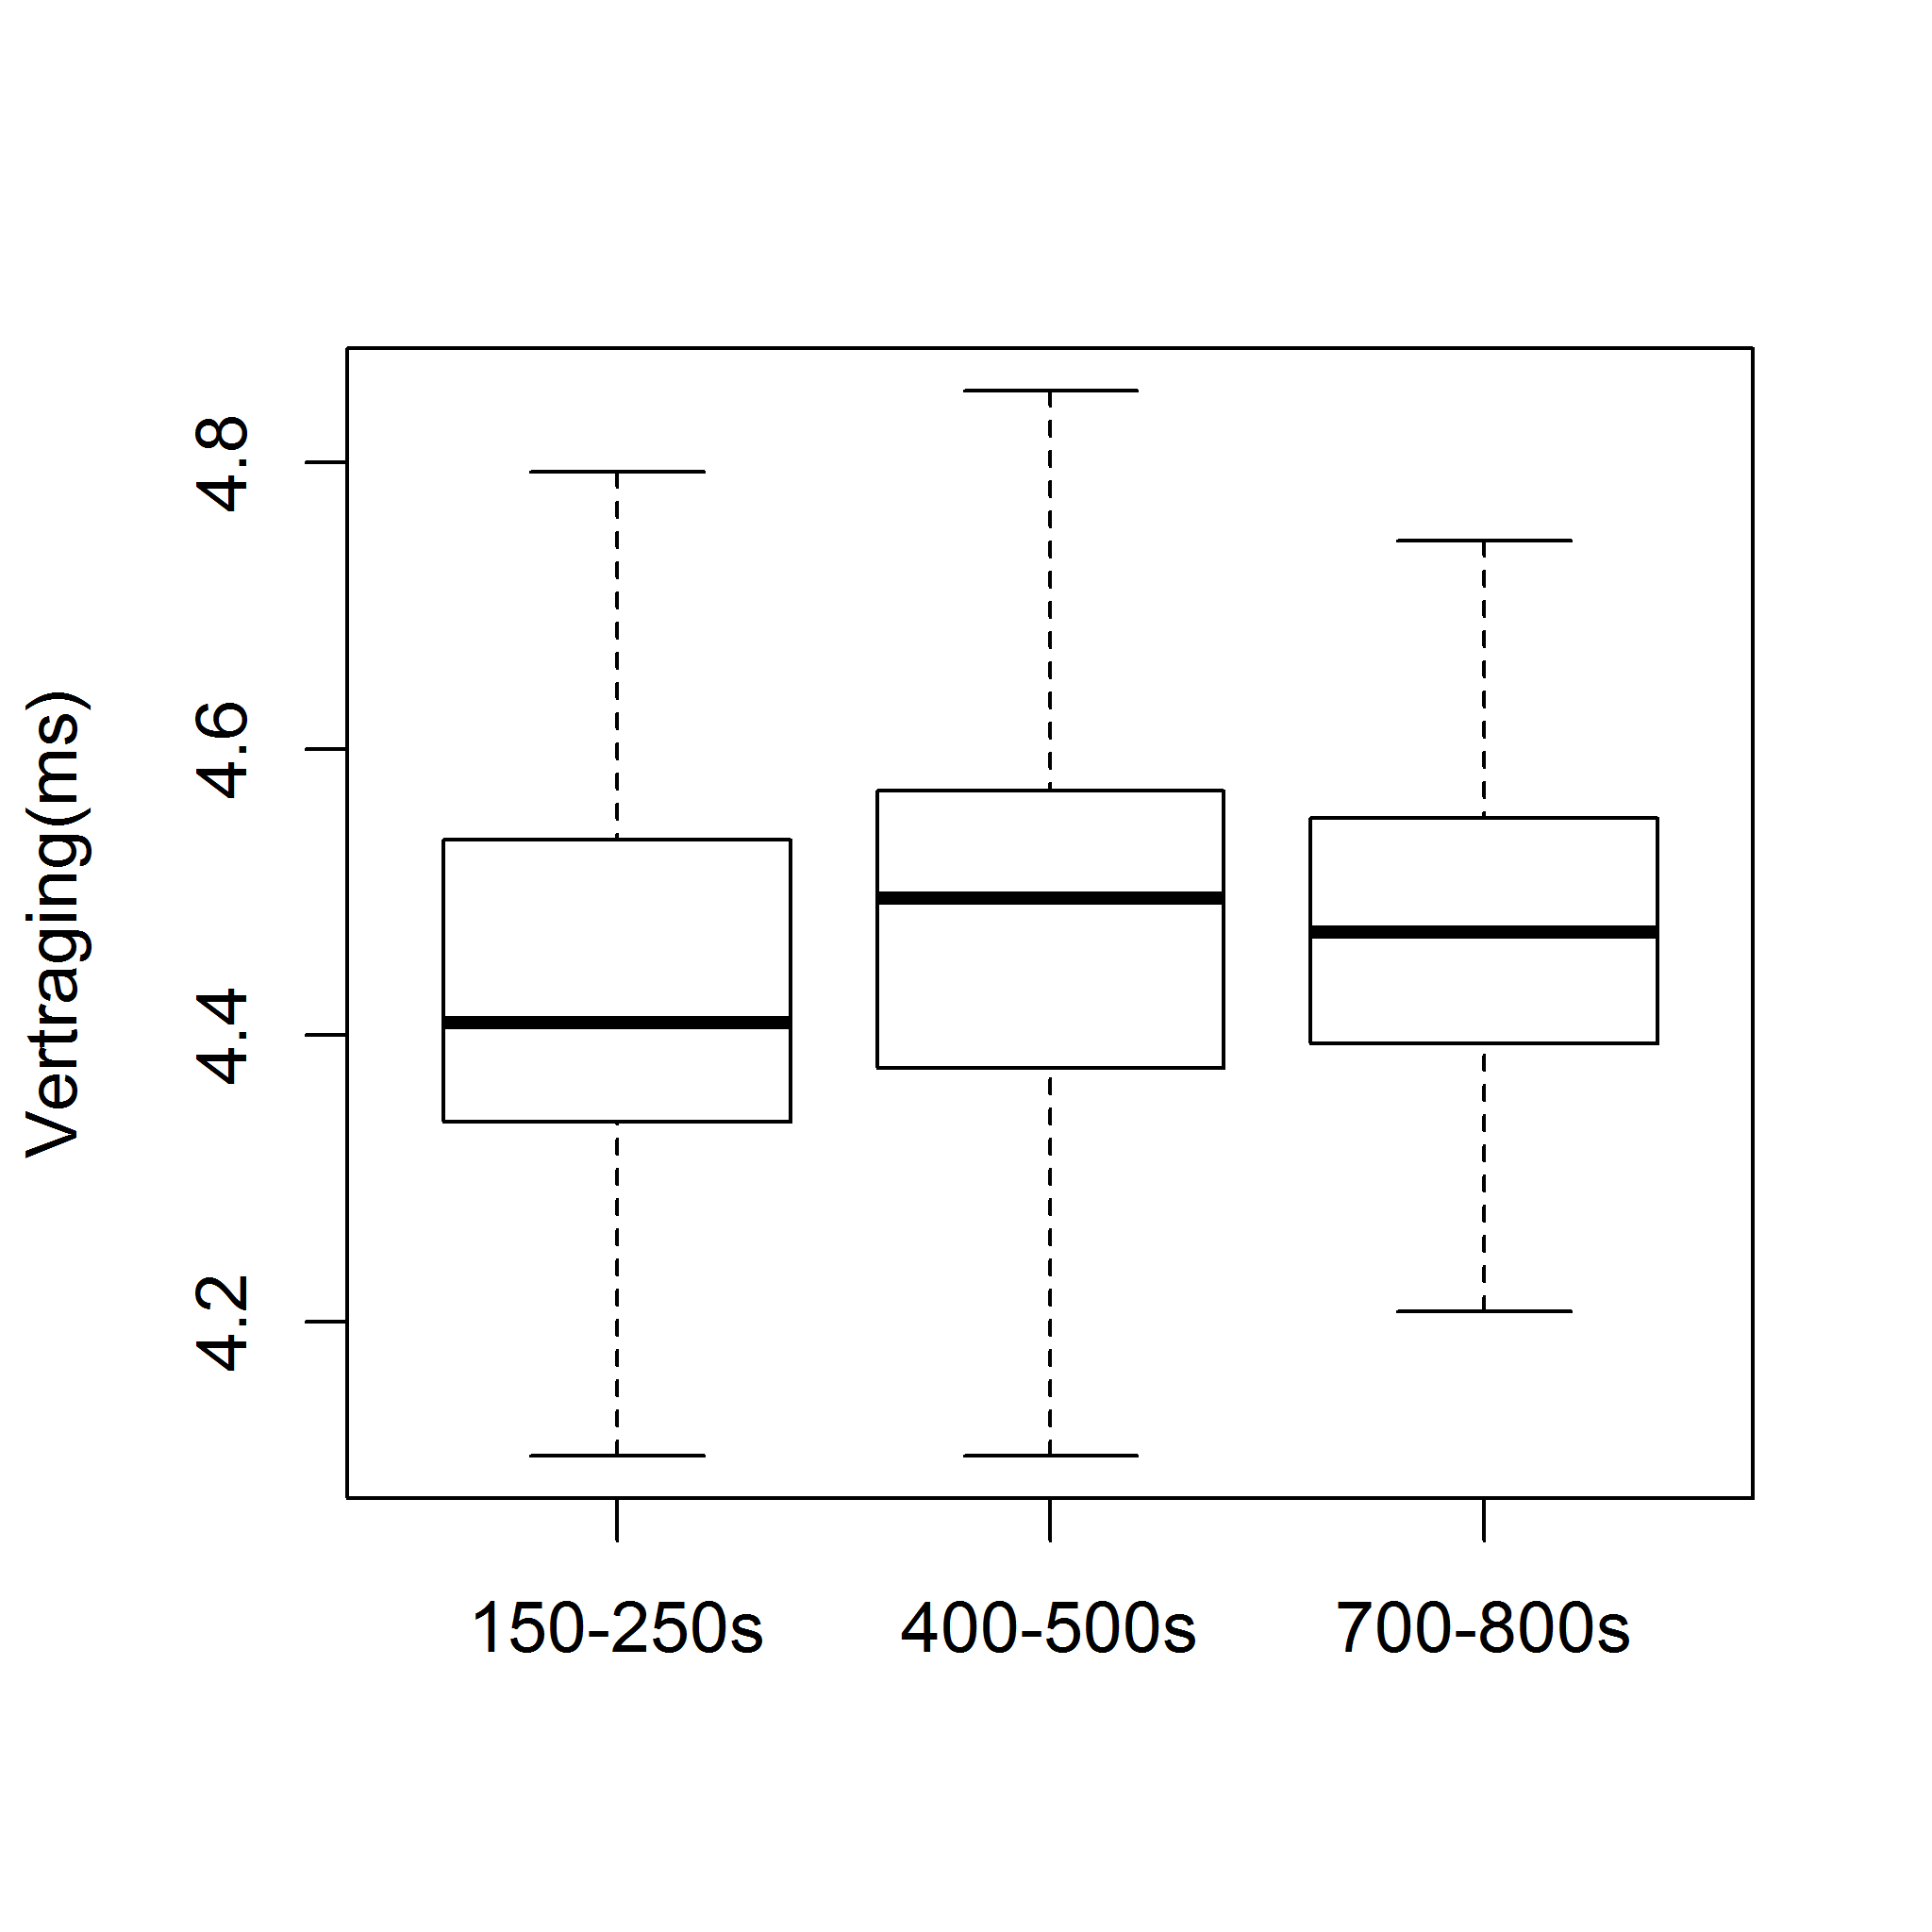
\includegraphics[width=0.45\textwidth]{img/Observaties/Pgpool/boxplot-graph-Node-1-READ}}
	\subfigure[Boxplot met schrijf vertragingen]{\label{fig:beschikbaar-pgpool-boxplot-write} 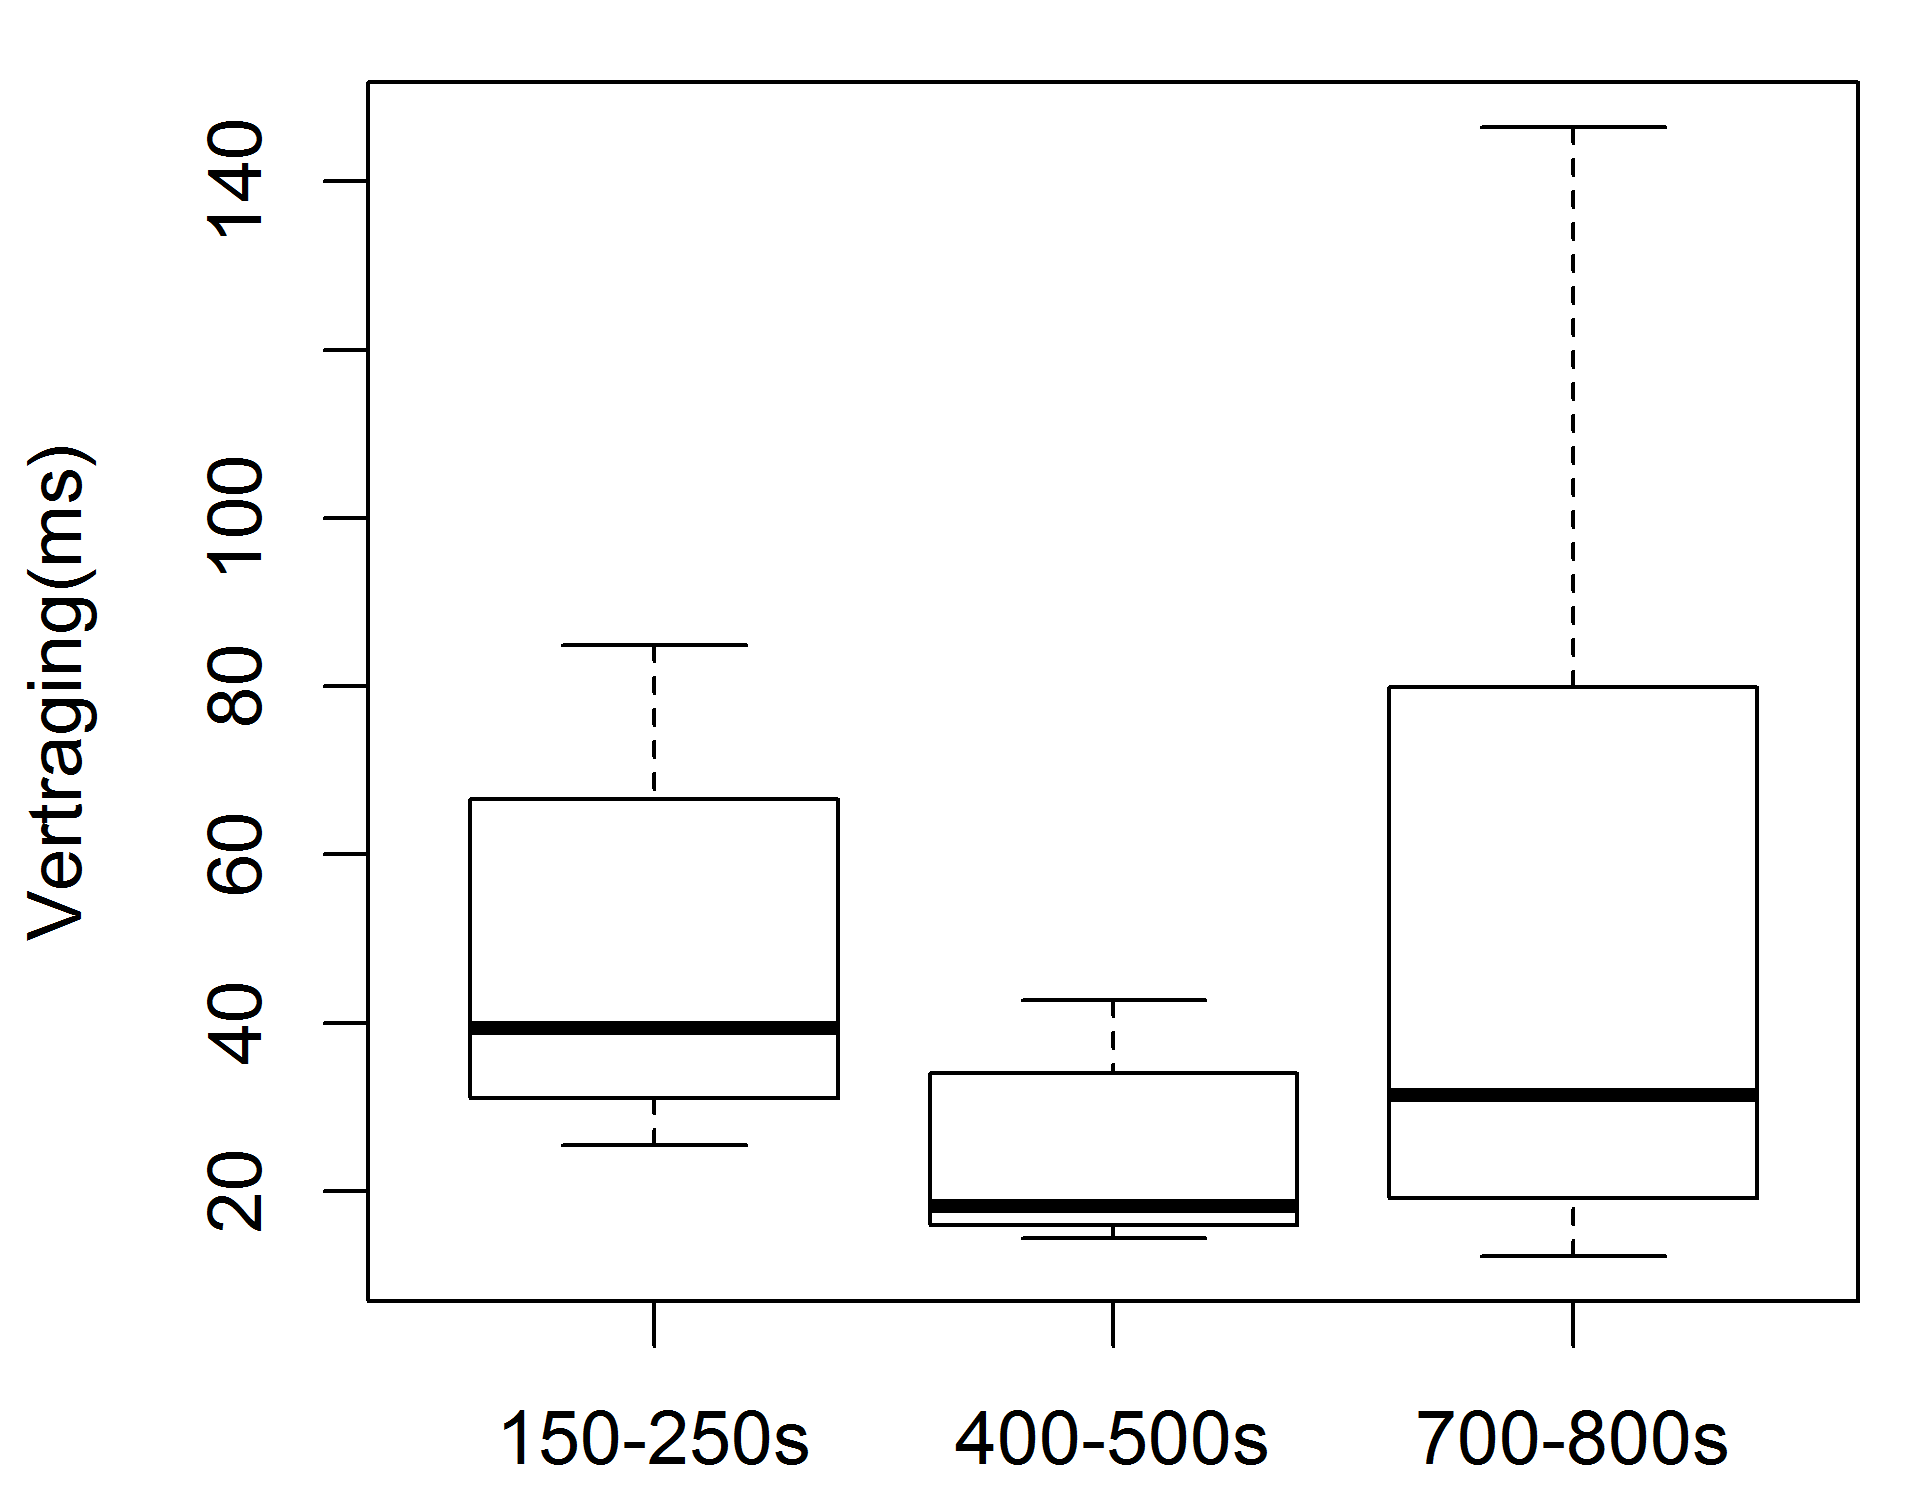
\includegraphics[width=0.45\textwidth]{img/Observaties/Pgpool/boxplot-graph-Node-1-UPDATE}}
	\caption{Beschikbaarheid: Verschillende voorbeeldreacties van MongoDB op beschikbaarheidstesten }
	\label{fig:beschikbaar-pgpool}
\end{figure}

\section{Consistentie test}
Voor de consistentie testen worden er empirische verdelingsfuncties gebruikt. Dit zijn functies waarbij op de x-as een waarde verloop is en op de y-as het percentage van de waarden kleiner dan x staat aangegeven.

Voor de consistentie testen wordt er op de x-as de start- en/of stoptijdstippen van de verschillende soorten getoond. Het verschil tussen de y-waarde van de start- en stoptijdstippen geeft aan hoeveel queries er op dat moment uitgevoerd worden. De startmomenten van een lezer zijn de eerste keer dat deze de correcte data leest.    

\paragraph{HBase}
Bij HBase is er geen verschil tussen het invoegen of aanpassen van data naar consistentie, dit zijn dezelfde queries. Daarnaast zijn er geen configuratie mogelijkheden voor het lezen of schrijven van data naast het in- of uitschakelen van de caches aan de gebruikerskant. 

Figuur \ref{fig:consistentie-hbase-start} toont een overzicht van de verschillende starttijdstippen voor het lezen van consistente data. Figuur \ref{fig:consistentie-hbase-R1} toont de start- en eindtijdstippen voor lezer 2 naast deze voor de schrijver. De maximale waarde van de x-as is zo gekozen dat voor elke dataset minstens 99\% van de data getoond is. 

\begin{figure}[ht!] 
	\centering
	\subfigure[Starttijdstippen van verschillende lezers voor lezen van consistente data]{\label{fig:consistentie-hbase-start} 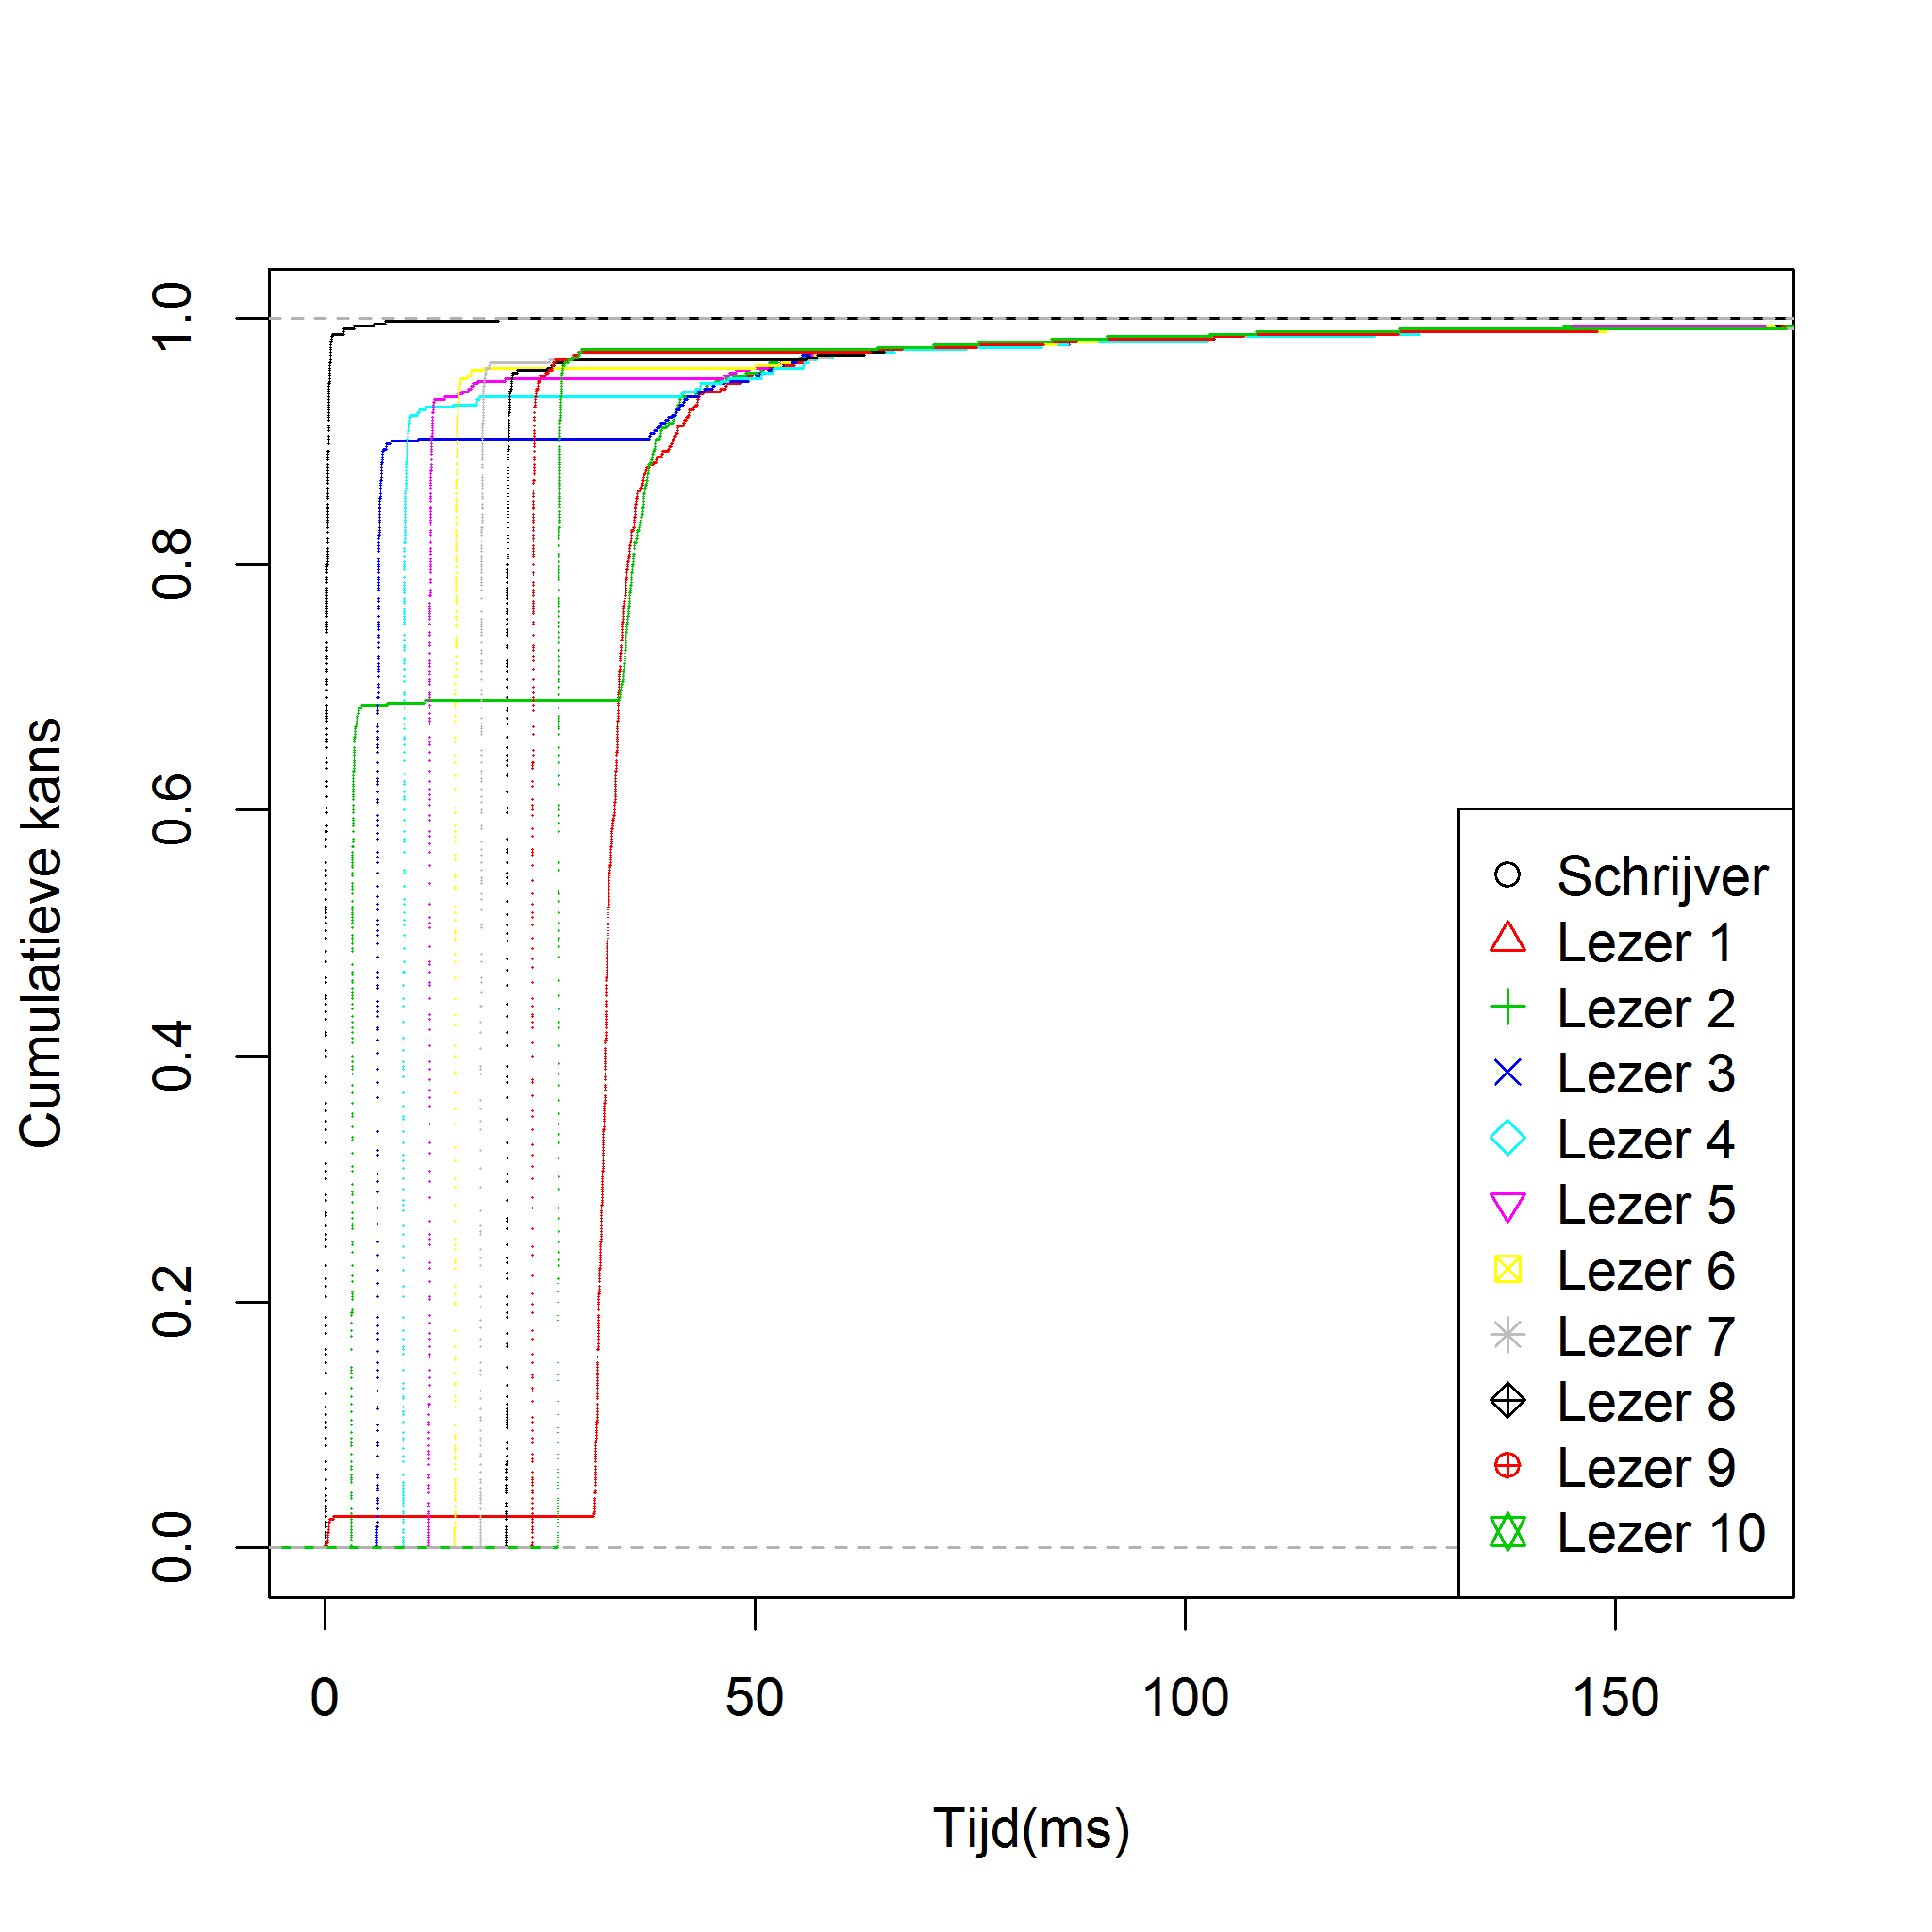
\includegraphics[width=.45\textwidth]{img/Observaties/HBase/ECDF-plot-Start-insertRawData-5}}
	\subfigure[De start- en stoptijdstippen voor lezer 2]{\label{fig:consistentie-hbase-R1} 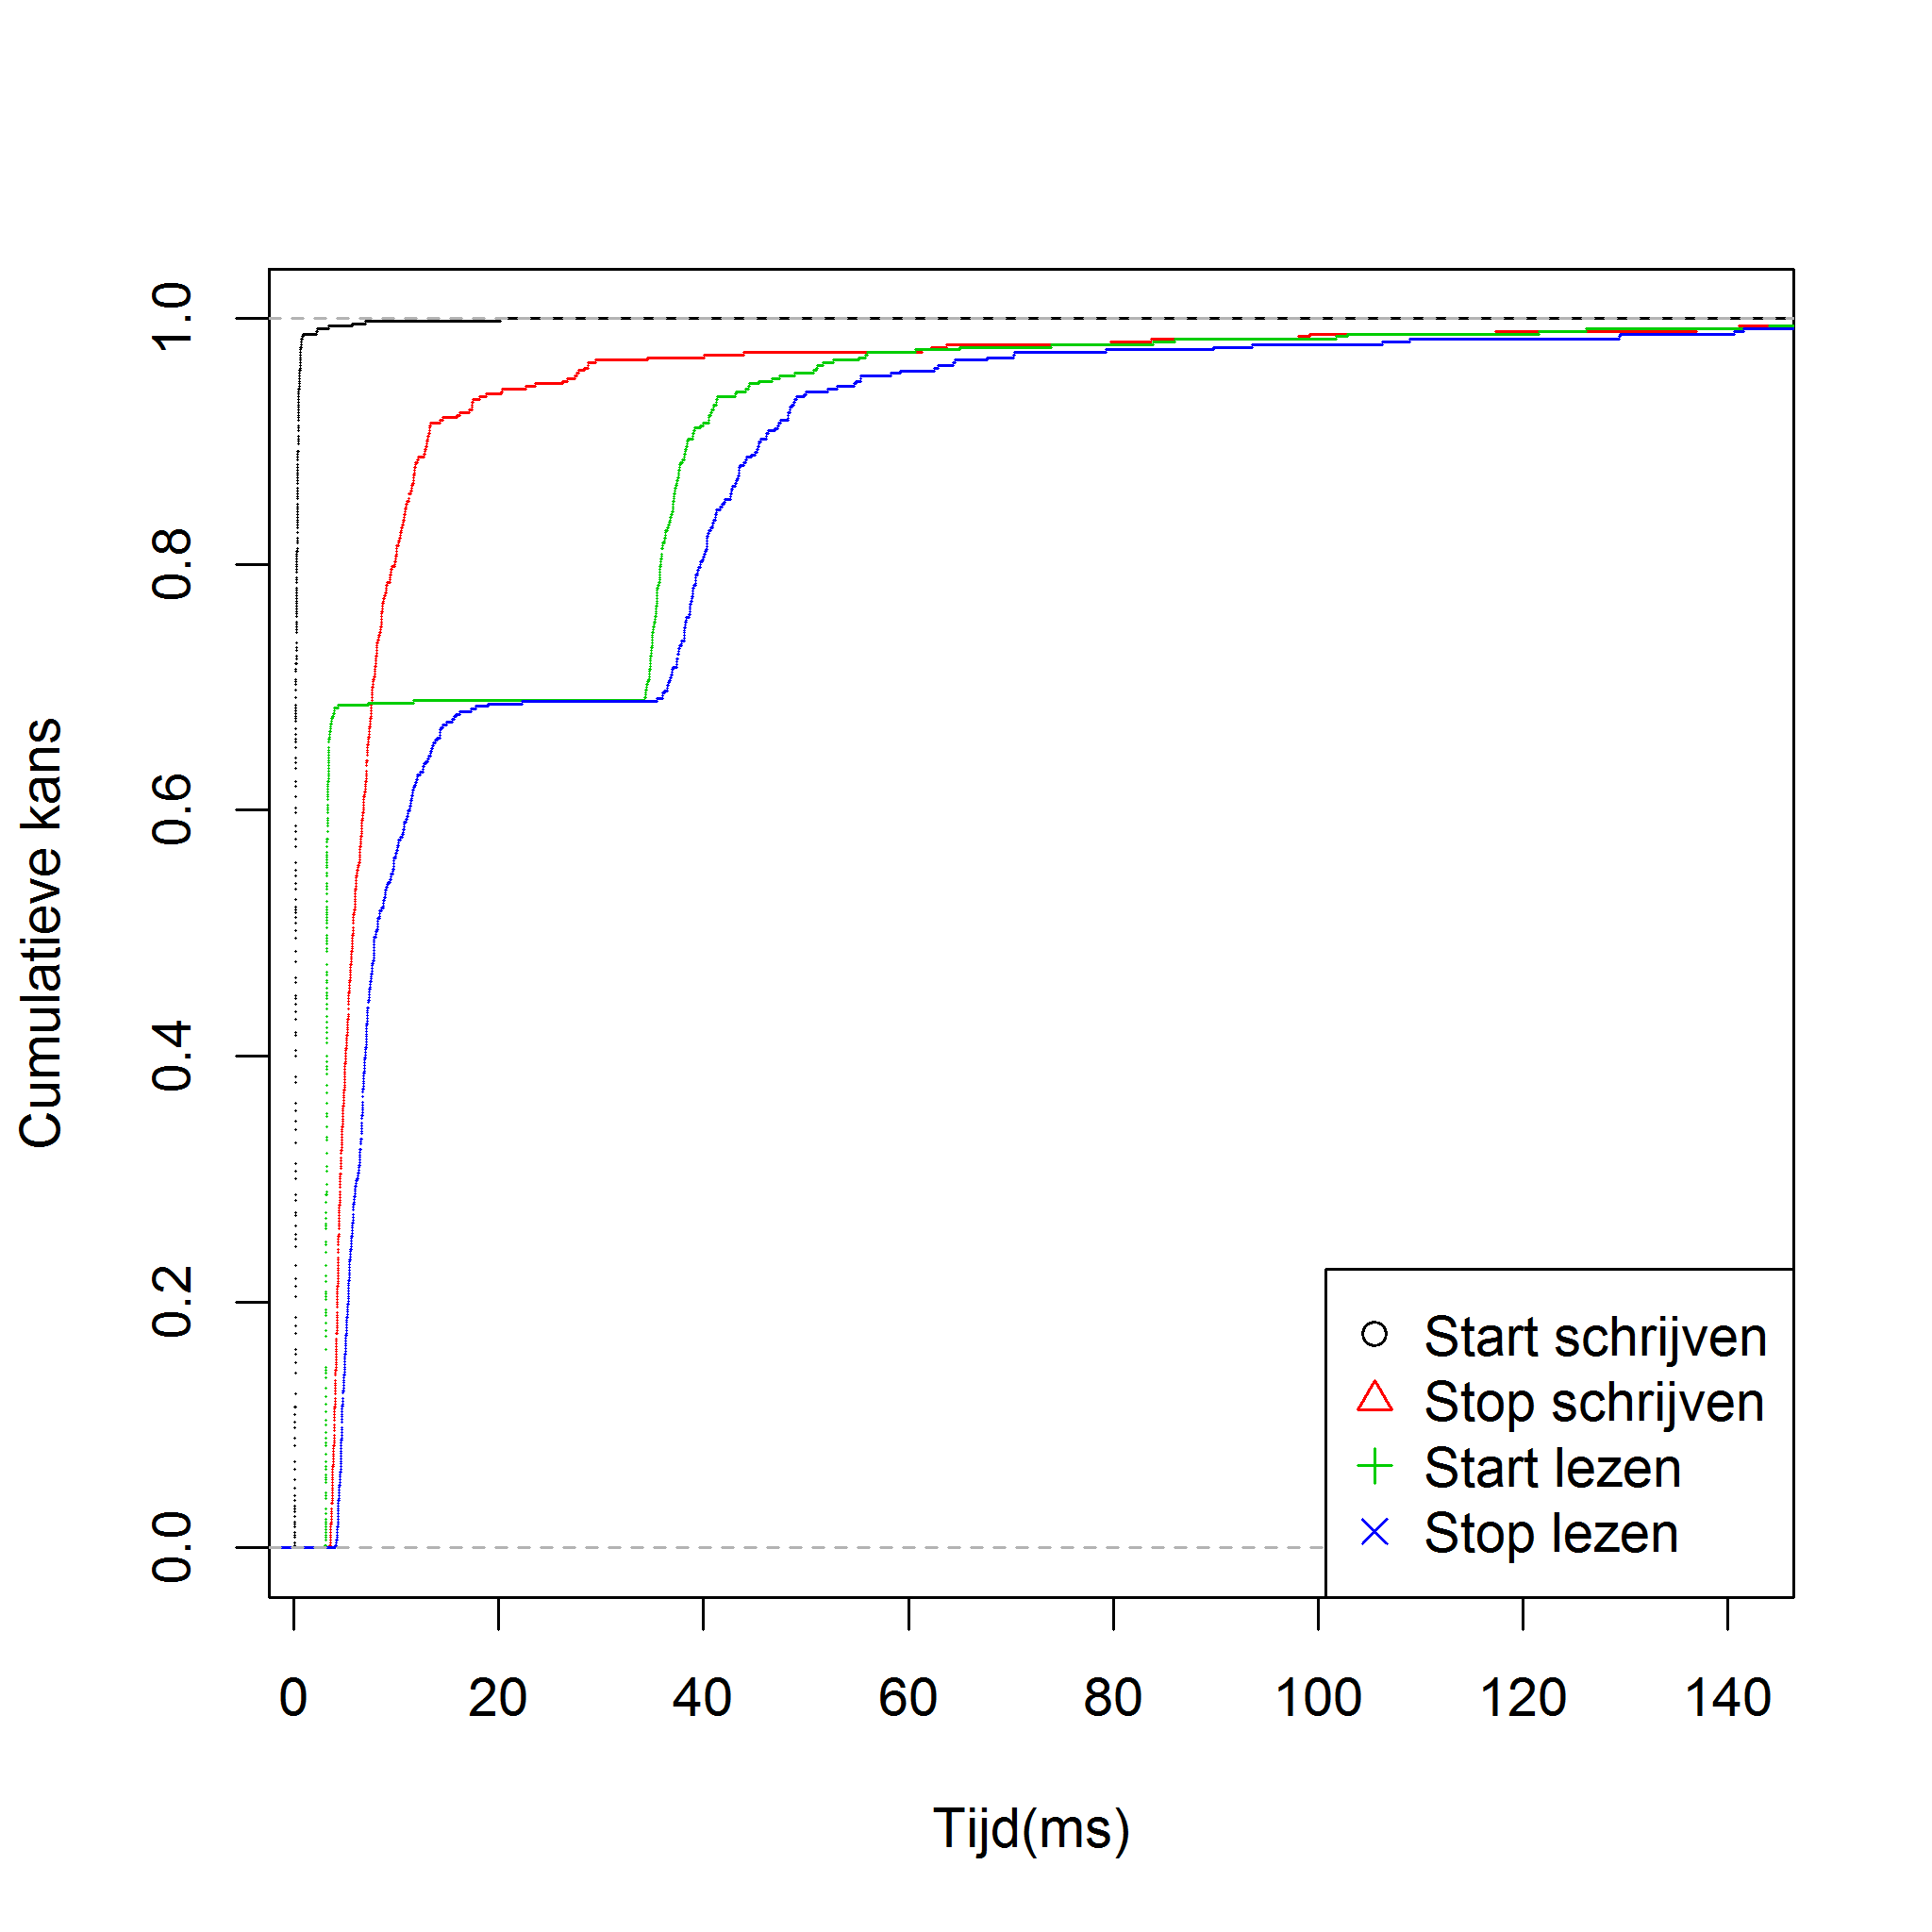
\includegraphics[width=0.45\textwidth]{img/Observaties/HBase/ECDF-plot-R-1-insertRawData-5}}

	\caption{Consistentie: Overzicht van HBase op de consistentie testen met een 99-percentiel.}
	\label{fig:consistentie-hbase}
\end{figure}

\paragraph{MongoDB} Bij MongoDB zijn er 5 soorten lees- en 5 soorten schrijfconfiguraties mogelijk. Na de testen bleek het dat secondarypreferred gelijk was aan secondary en is niet getoond in de grafieken om deze reden. 

Voor elk van de 5 mogelijke schrijvacties, is een overzicht gegeven in figuren \ref{fig:consistentie-mongodb-all} en \ref{fig:consistentie-mongodb-R2}. In de eerste figuur, is de data van al de lezers gecombineerd, bij de tweede wordt er enkel naar lezer 2 gekeken. De maximale waarde van de x-as is zo gekozen dat voor elke dataset minstens 97\% en 99\% van de data getoond is voor respectievelijk figuur \ref{fig:consistentie-mongodb-all} en \ref{fig:consistentie-mongodb-R2}. Er zijn telkens de update queries getoond met een vergelijking tussen de insert en update bij majority. Ook uit de andere data blijkt dat deze niet significant verschillend zijn. 

Een vergelijking van de duur van de verschillende leesoperaties kan gevonden worden in figuur \ref{fig:consistentie-mongodb-all-mongodb-write} waar er minstens 90\% van de data is getoond. 

\begin{figure}[htb!] 
	\centering
	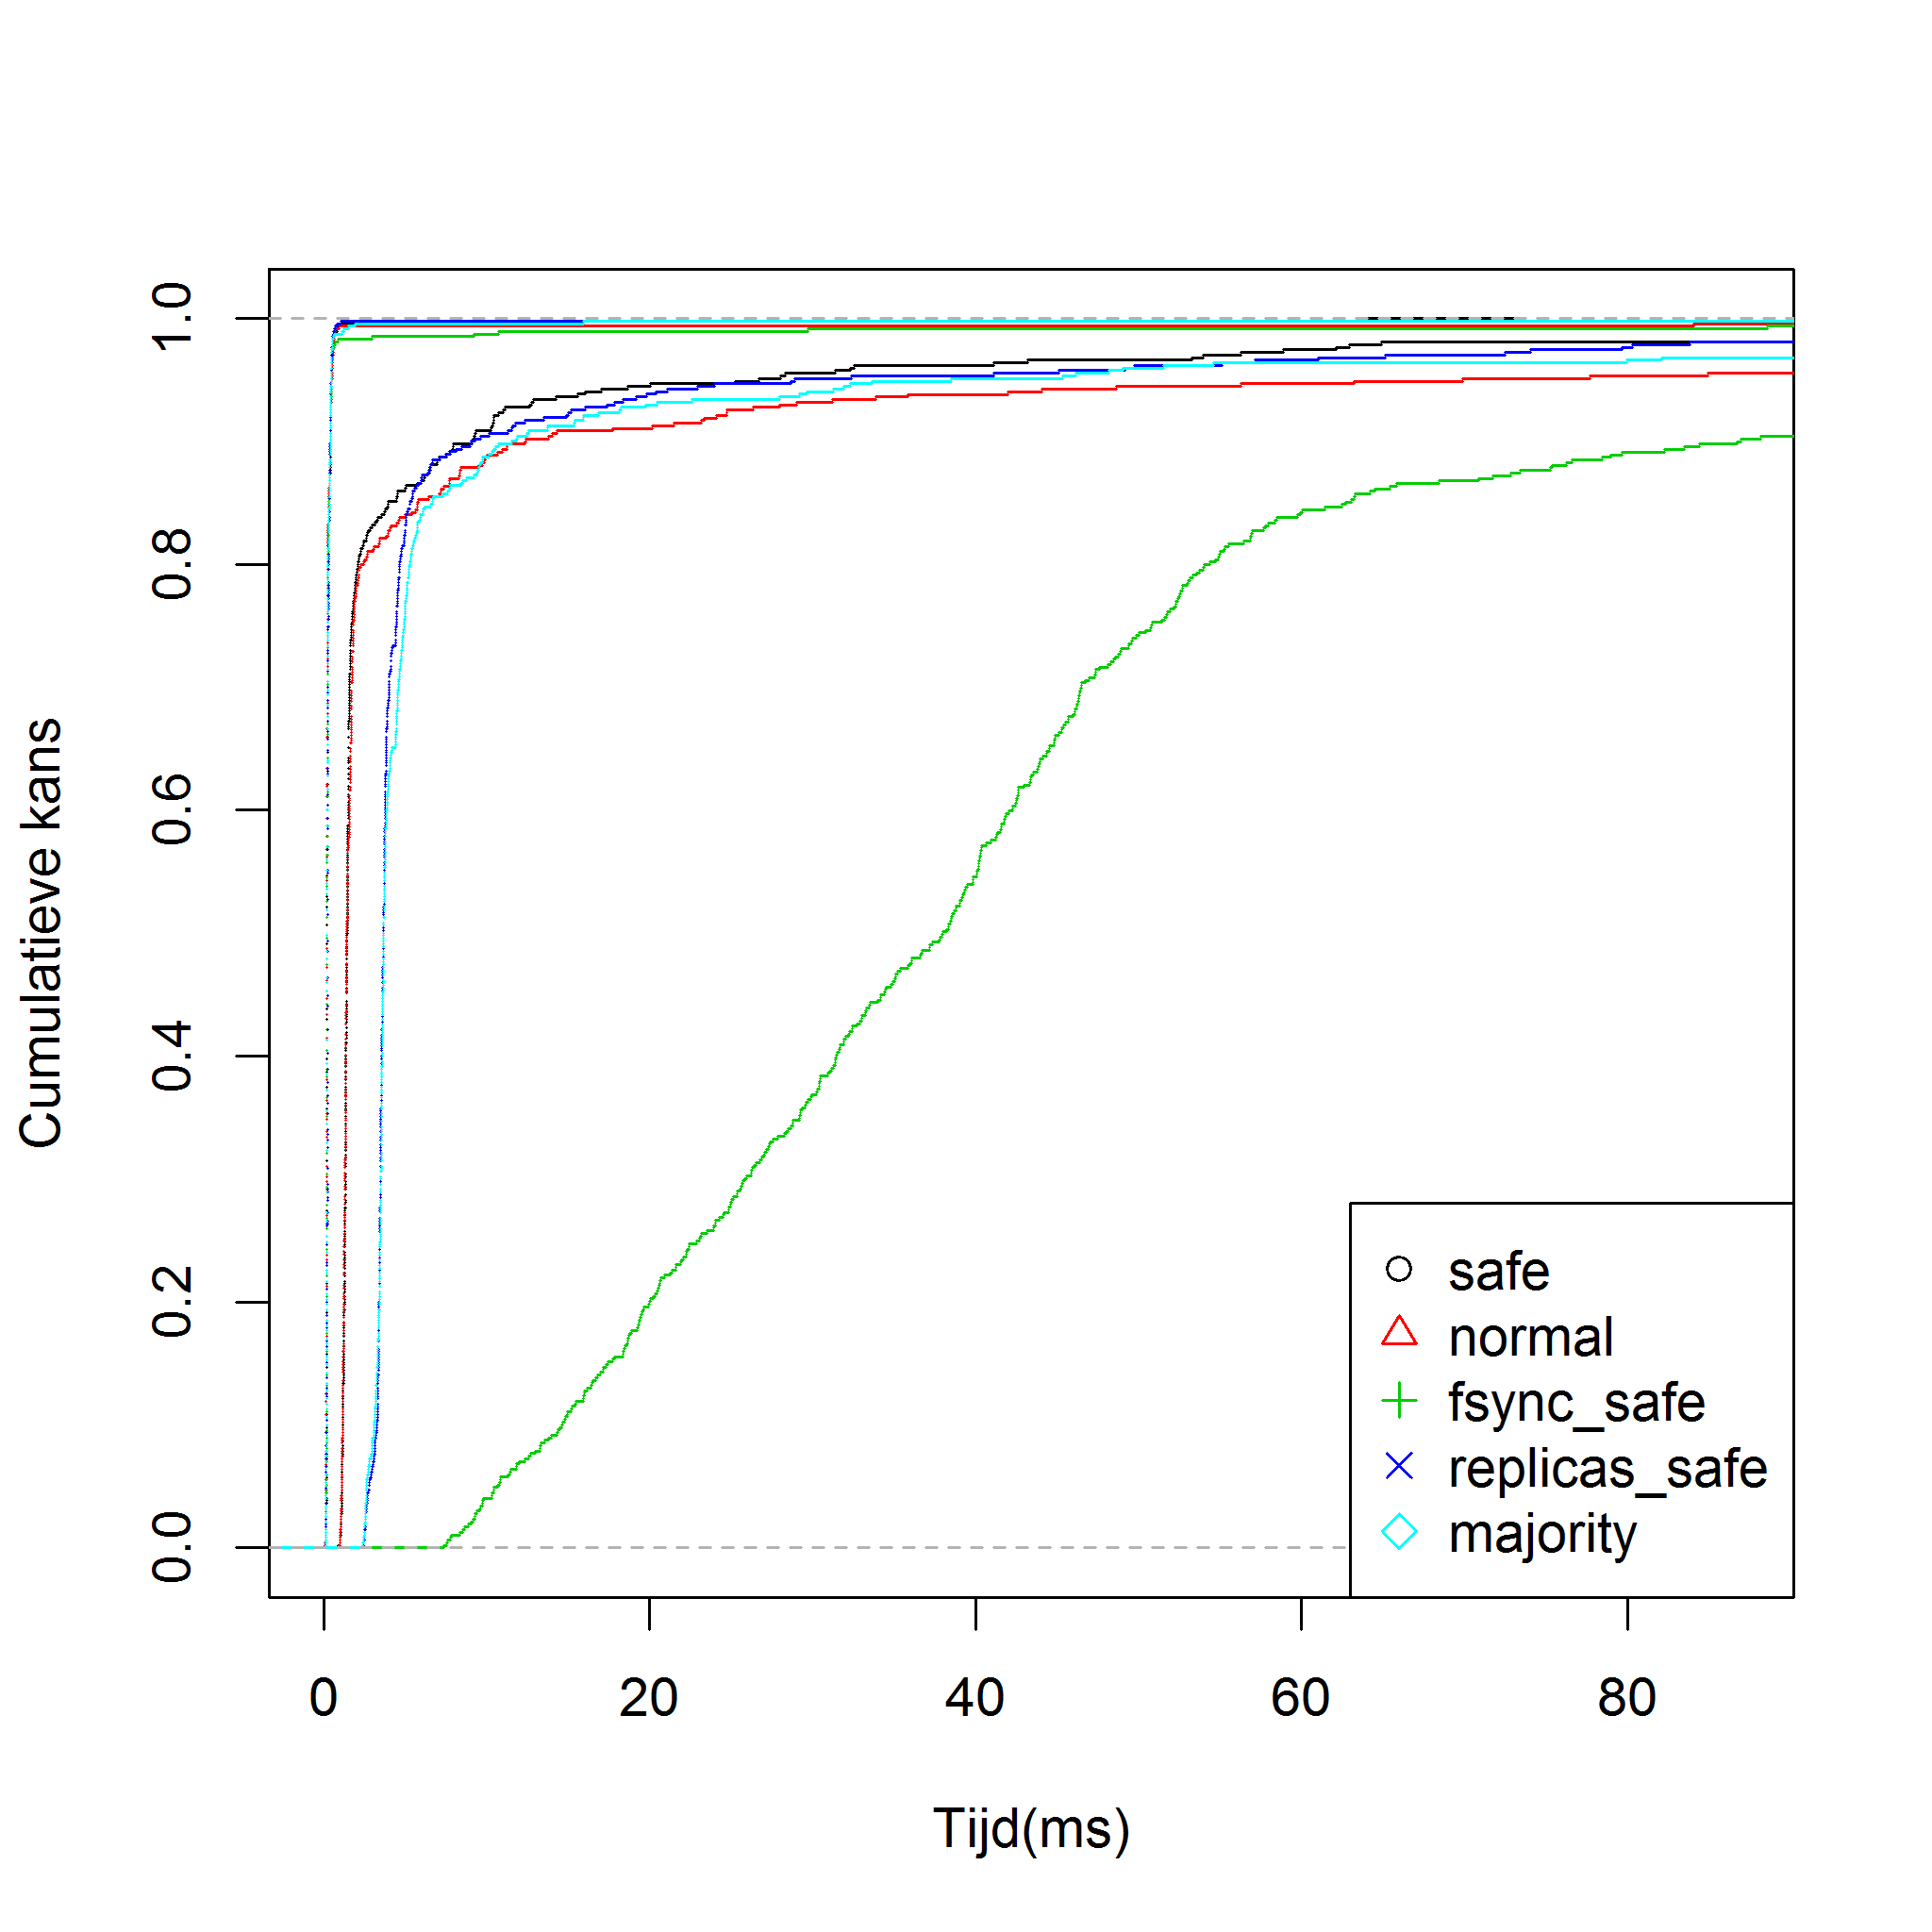
\includegraphics[width=.42\textwidth]{img/Observaties/MongoDB/ECDF-Compare-Write-insert-1}
	\caption{Consistentie: Overzicht van MongoDB's verschillende schrijfoperaties met een 90-percentiel. }
	\label{fig:consistentie-mongodb-all-mongodb-write}
\end{figure}

\begin{figure}[ht!] 
	\centering
	\subfigure[Normal Update]{\label{fig:consistentie-all-mongodb-normal} 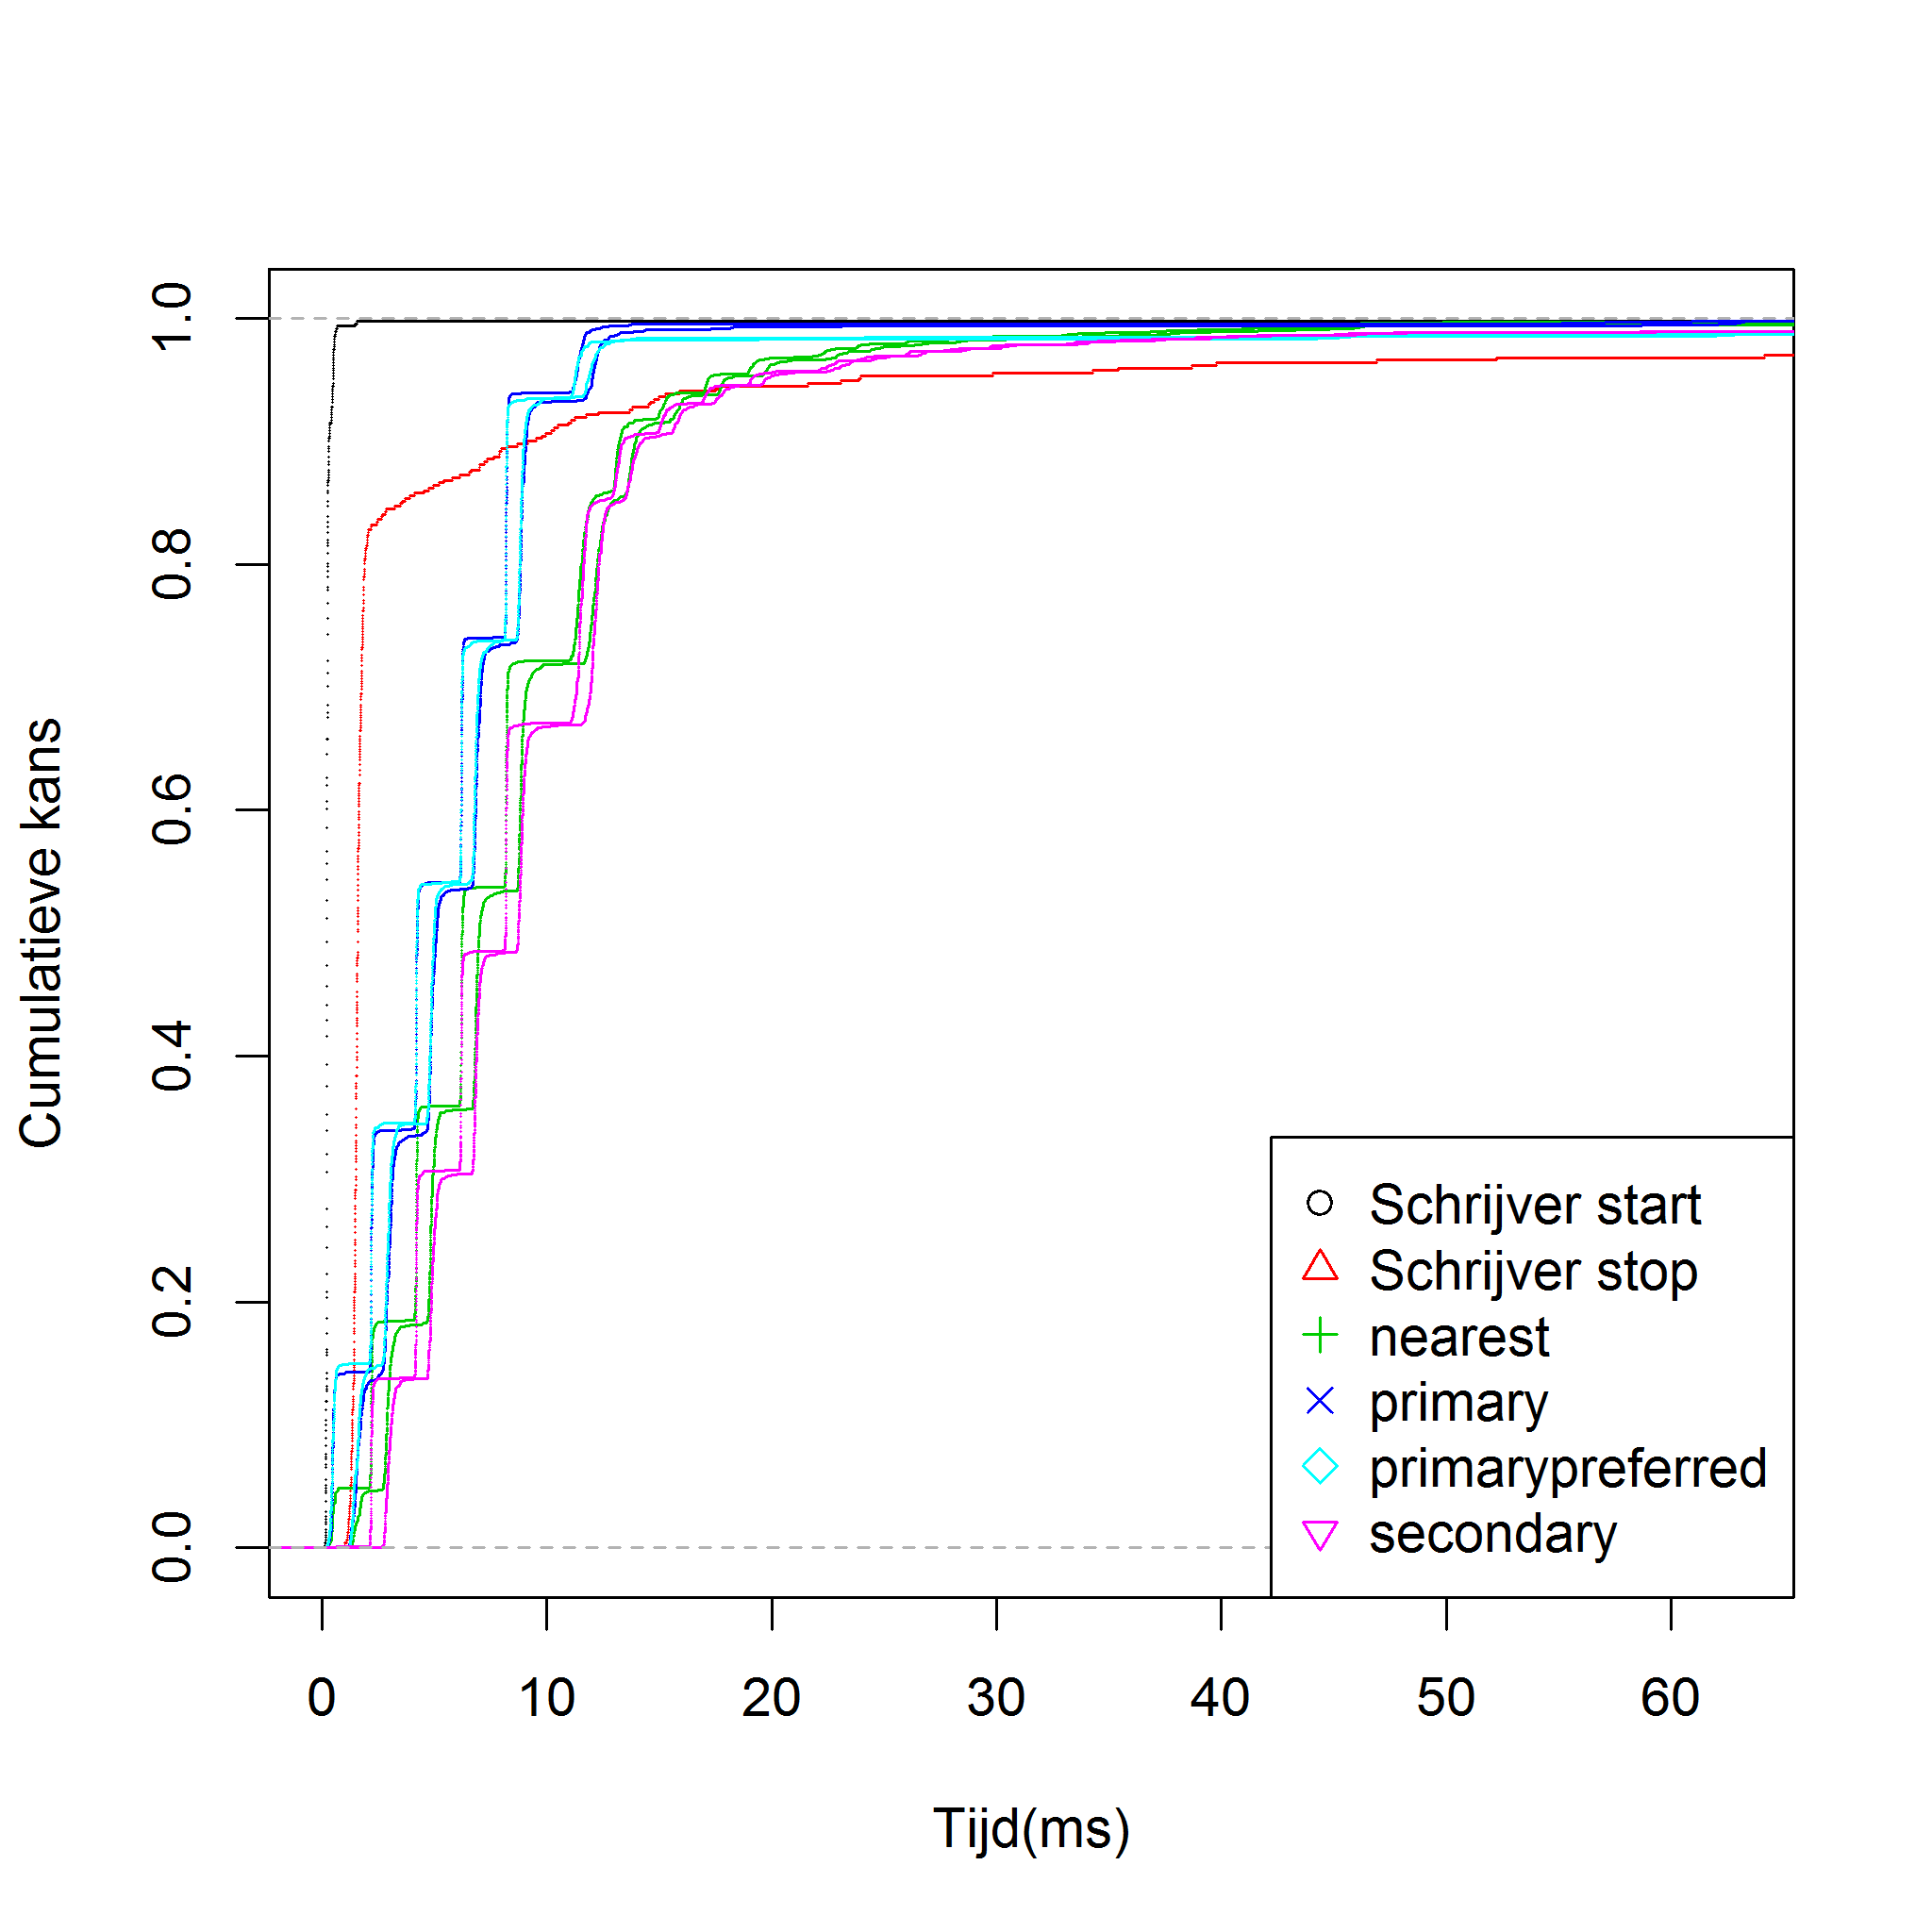
\includegraphics[width=.42\textwidth]{img/Observaties/MongoDB/ECDF-Reads-update-normal-all-2}}
	\subfigure[Safe Update]{\label{fig:consistentie-all-mongodb-safe} 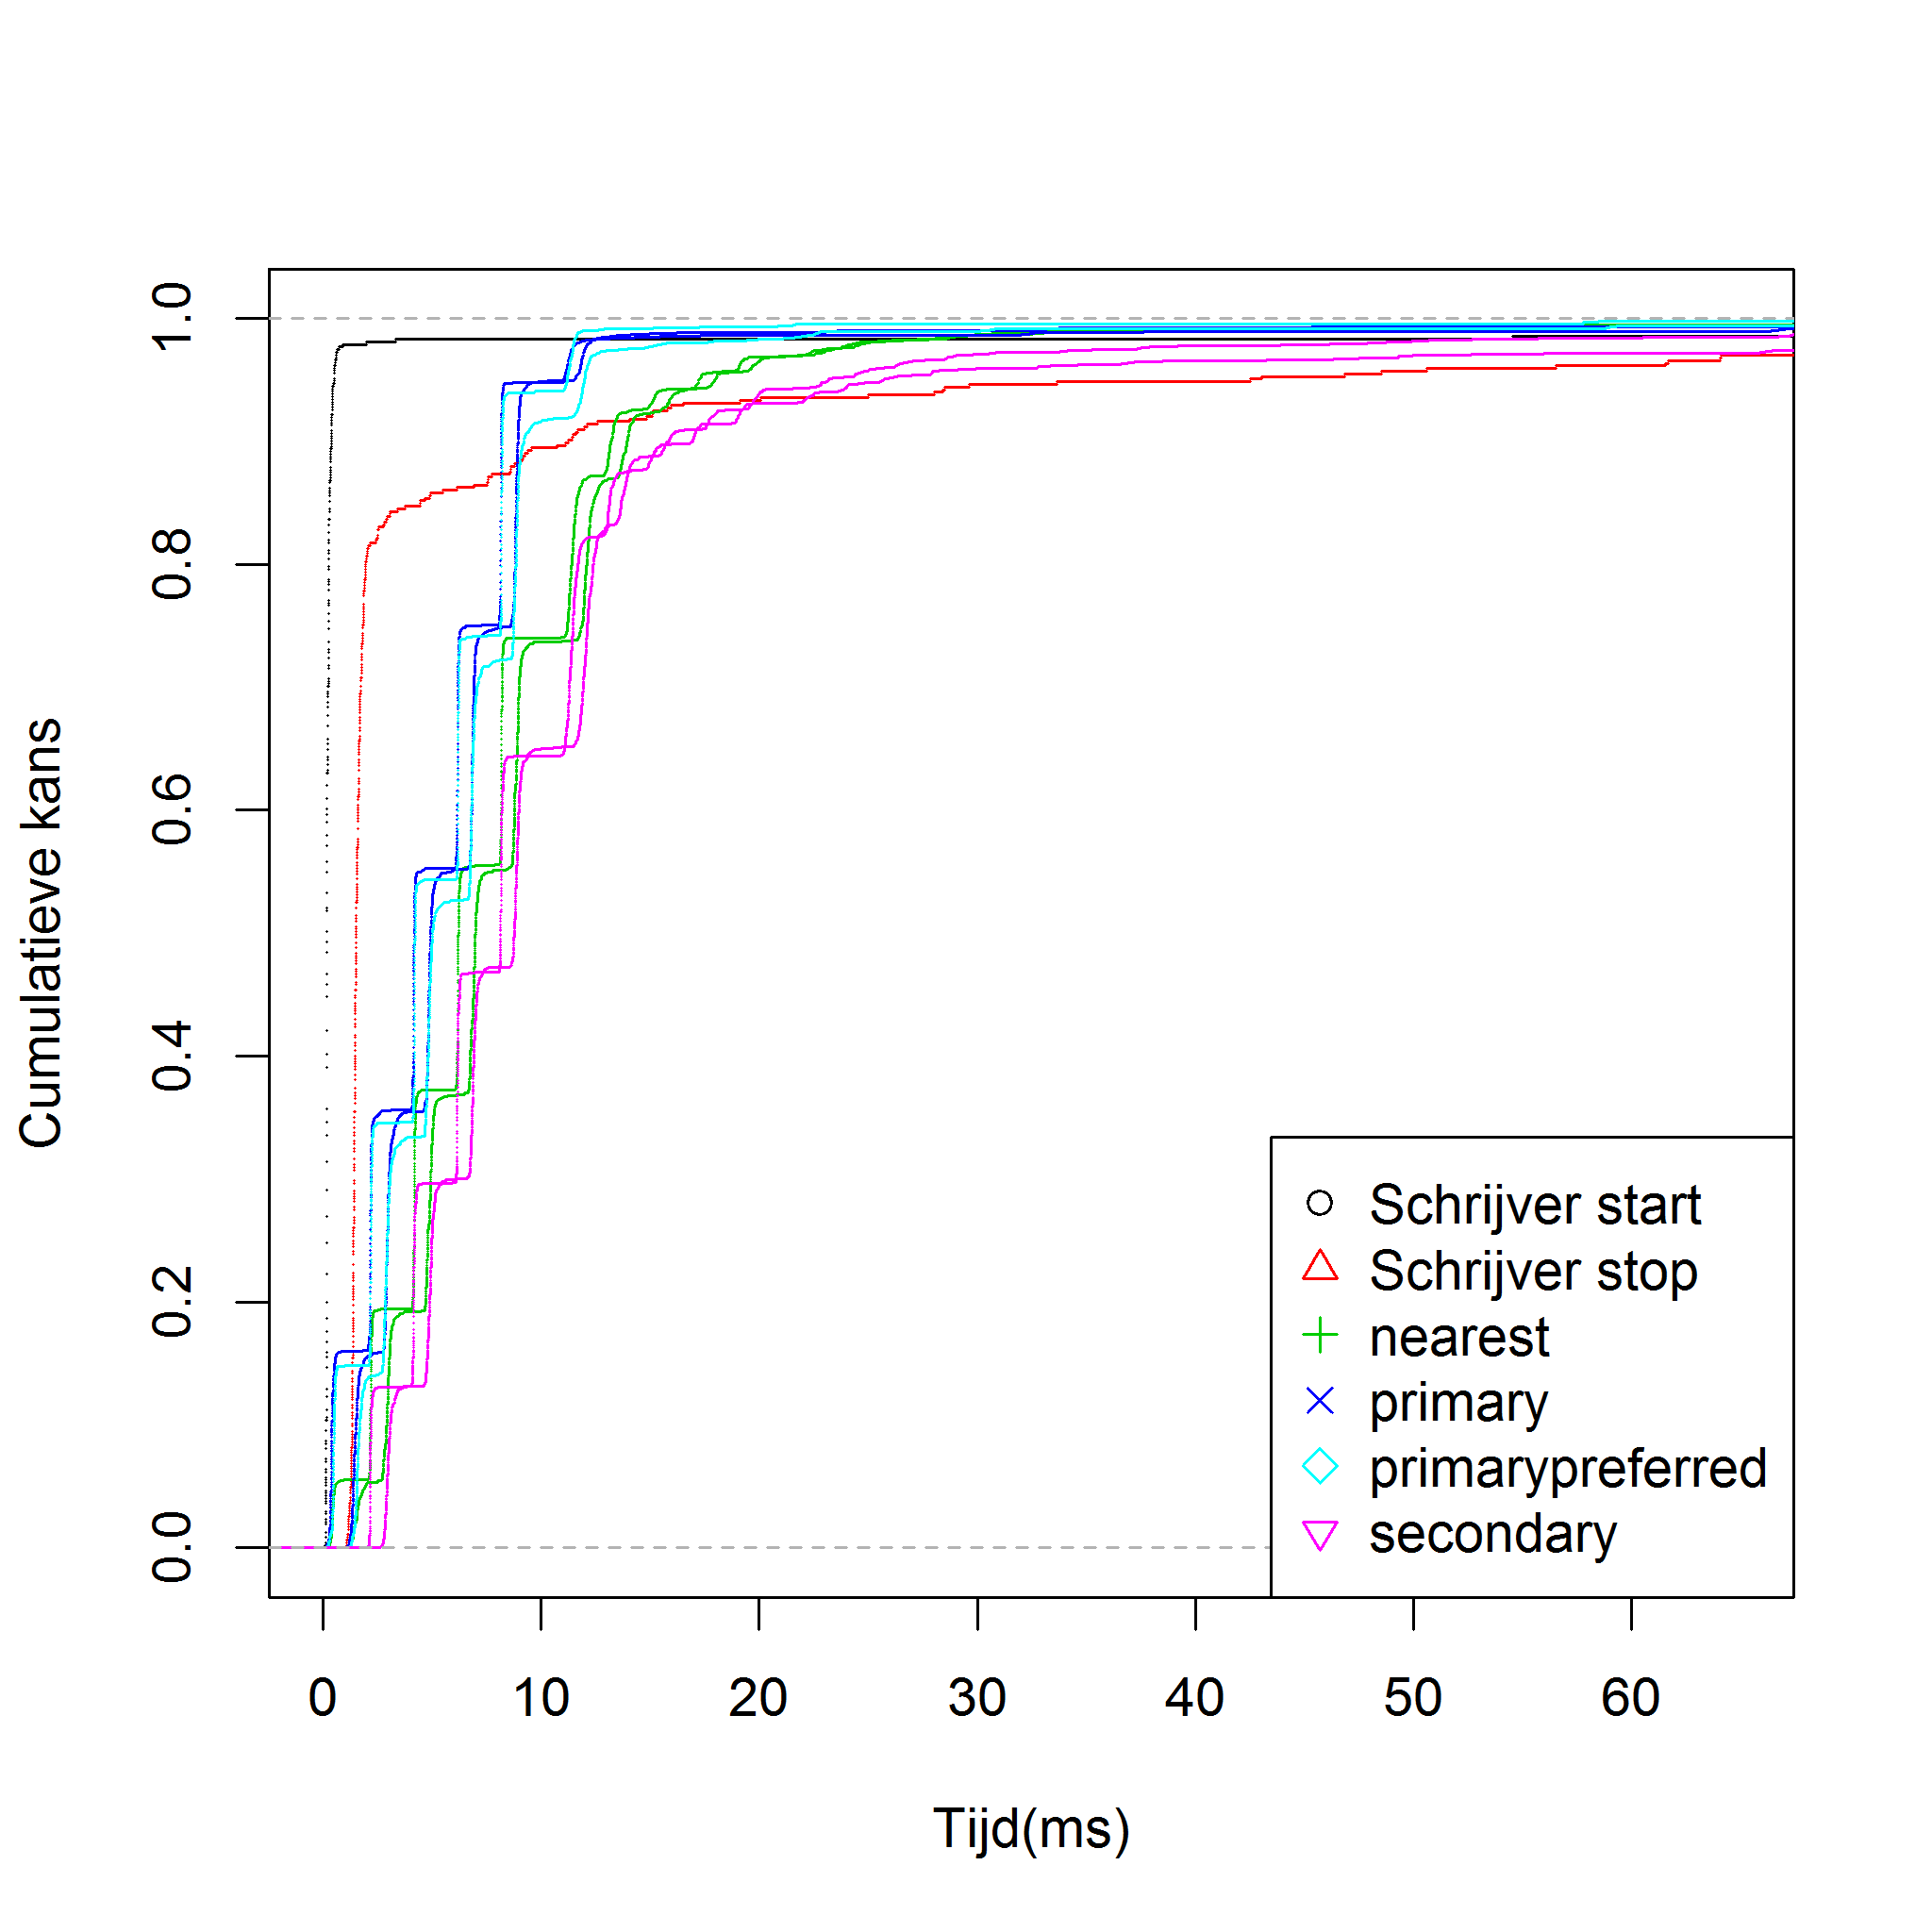
\includegraphics[width=.42\textwidth]{img/Observaties/MongoDB/ECDF-Reads-update-safe-all-2}}
	\subfigure[Fsync Safe Update]{\label{fig:consistentie-all-mongodb-fsync} 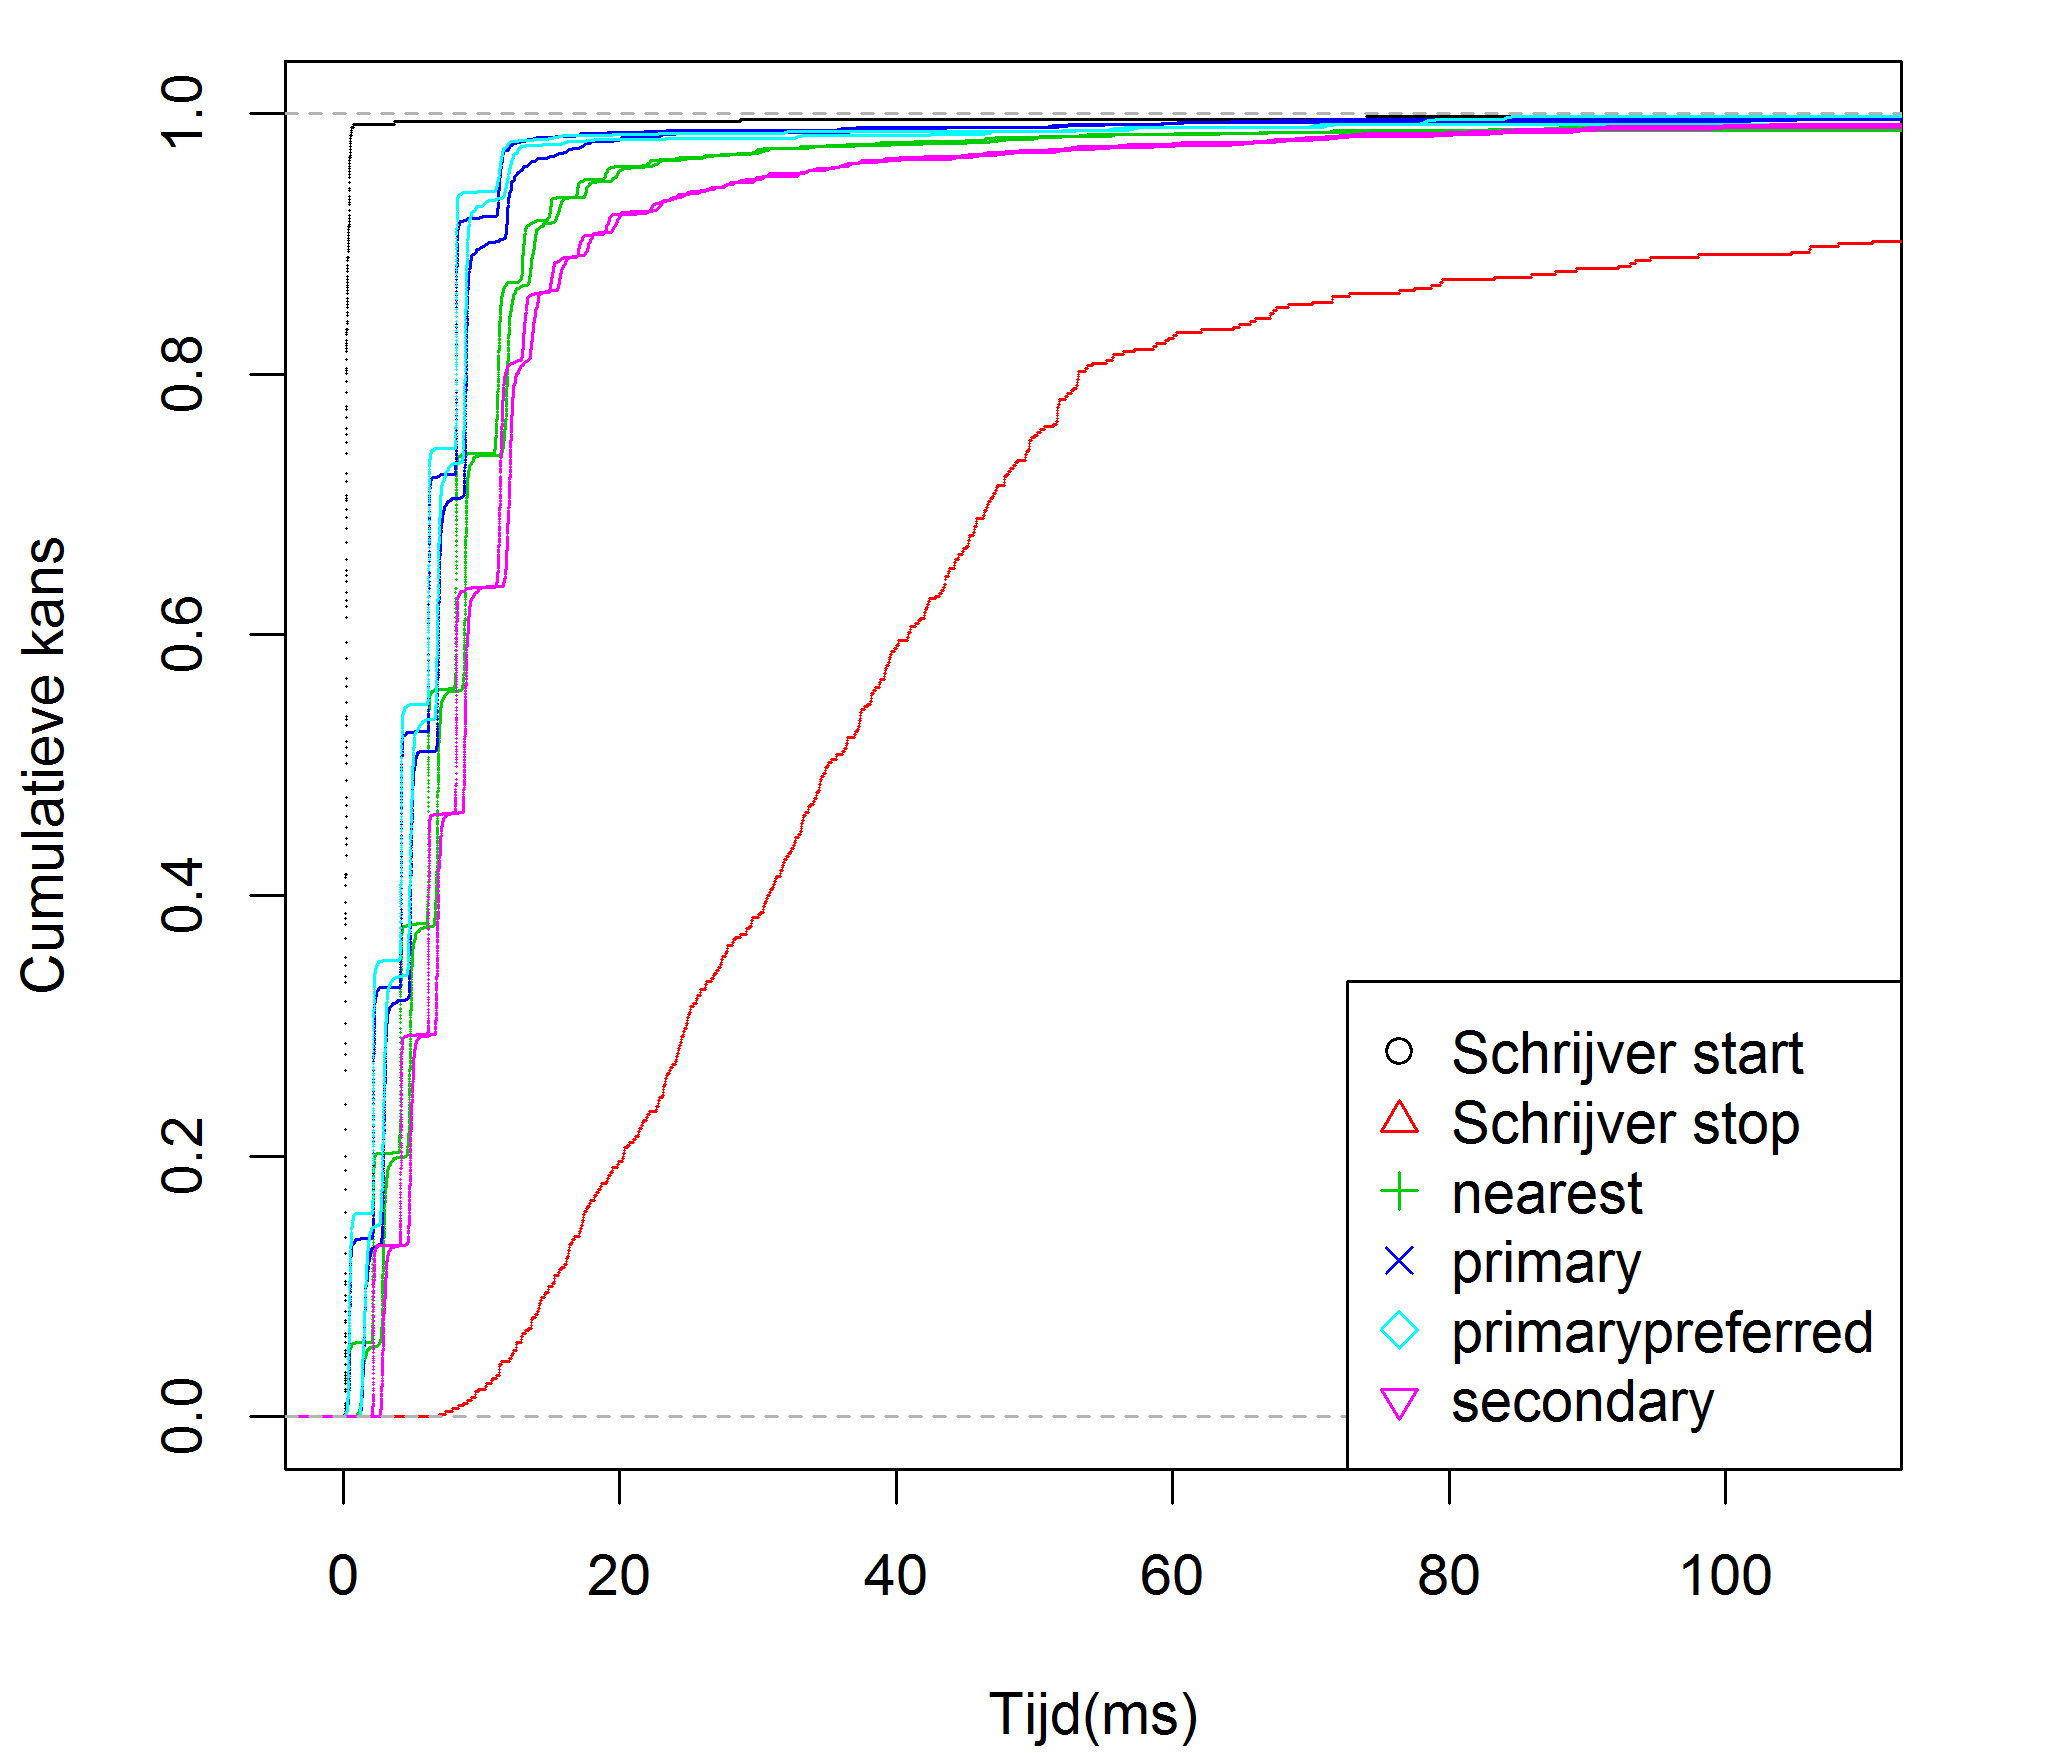
\includegraphics[width=.42\textwidth]{img/Observaties/MongoDB/ECDF-Reads-update-fsync_safe-all-2}}
	\subfigure[Replica Safe Update]{\label{fig:consistentie-all-mongodb-replicasafe} 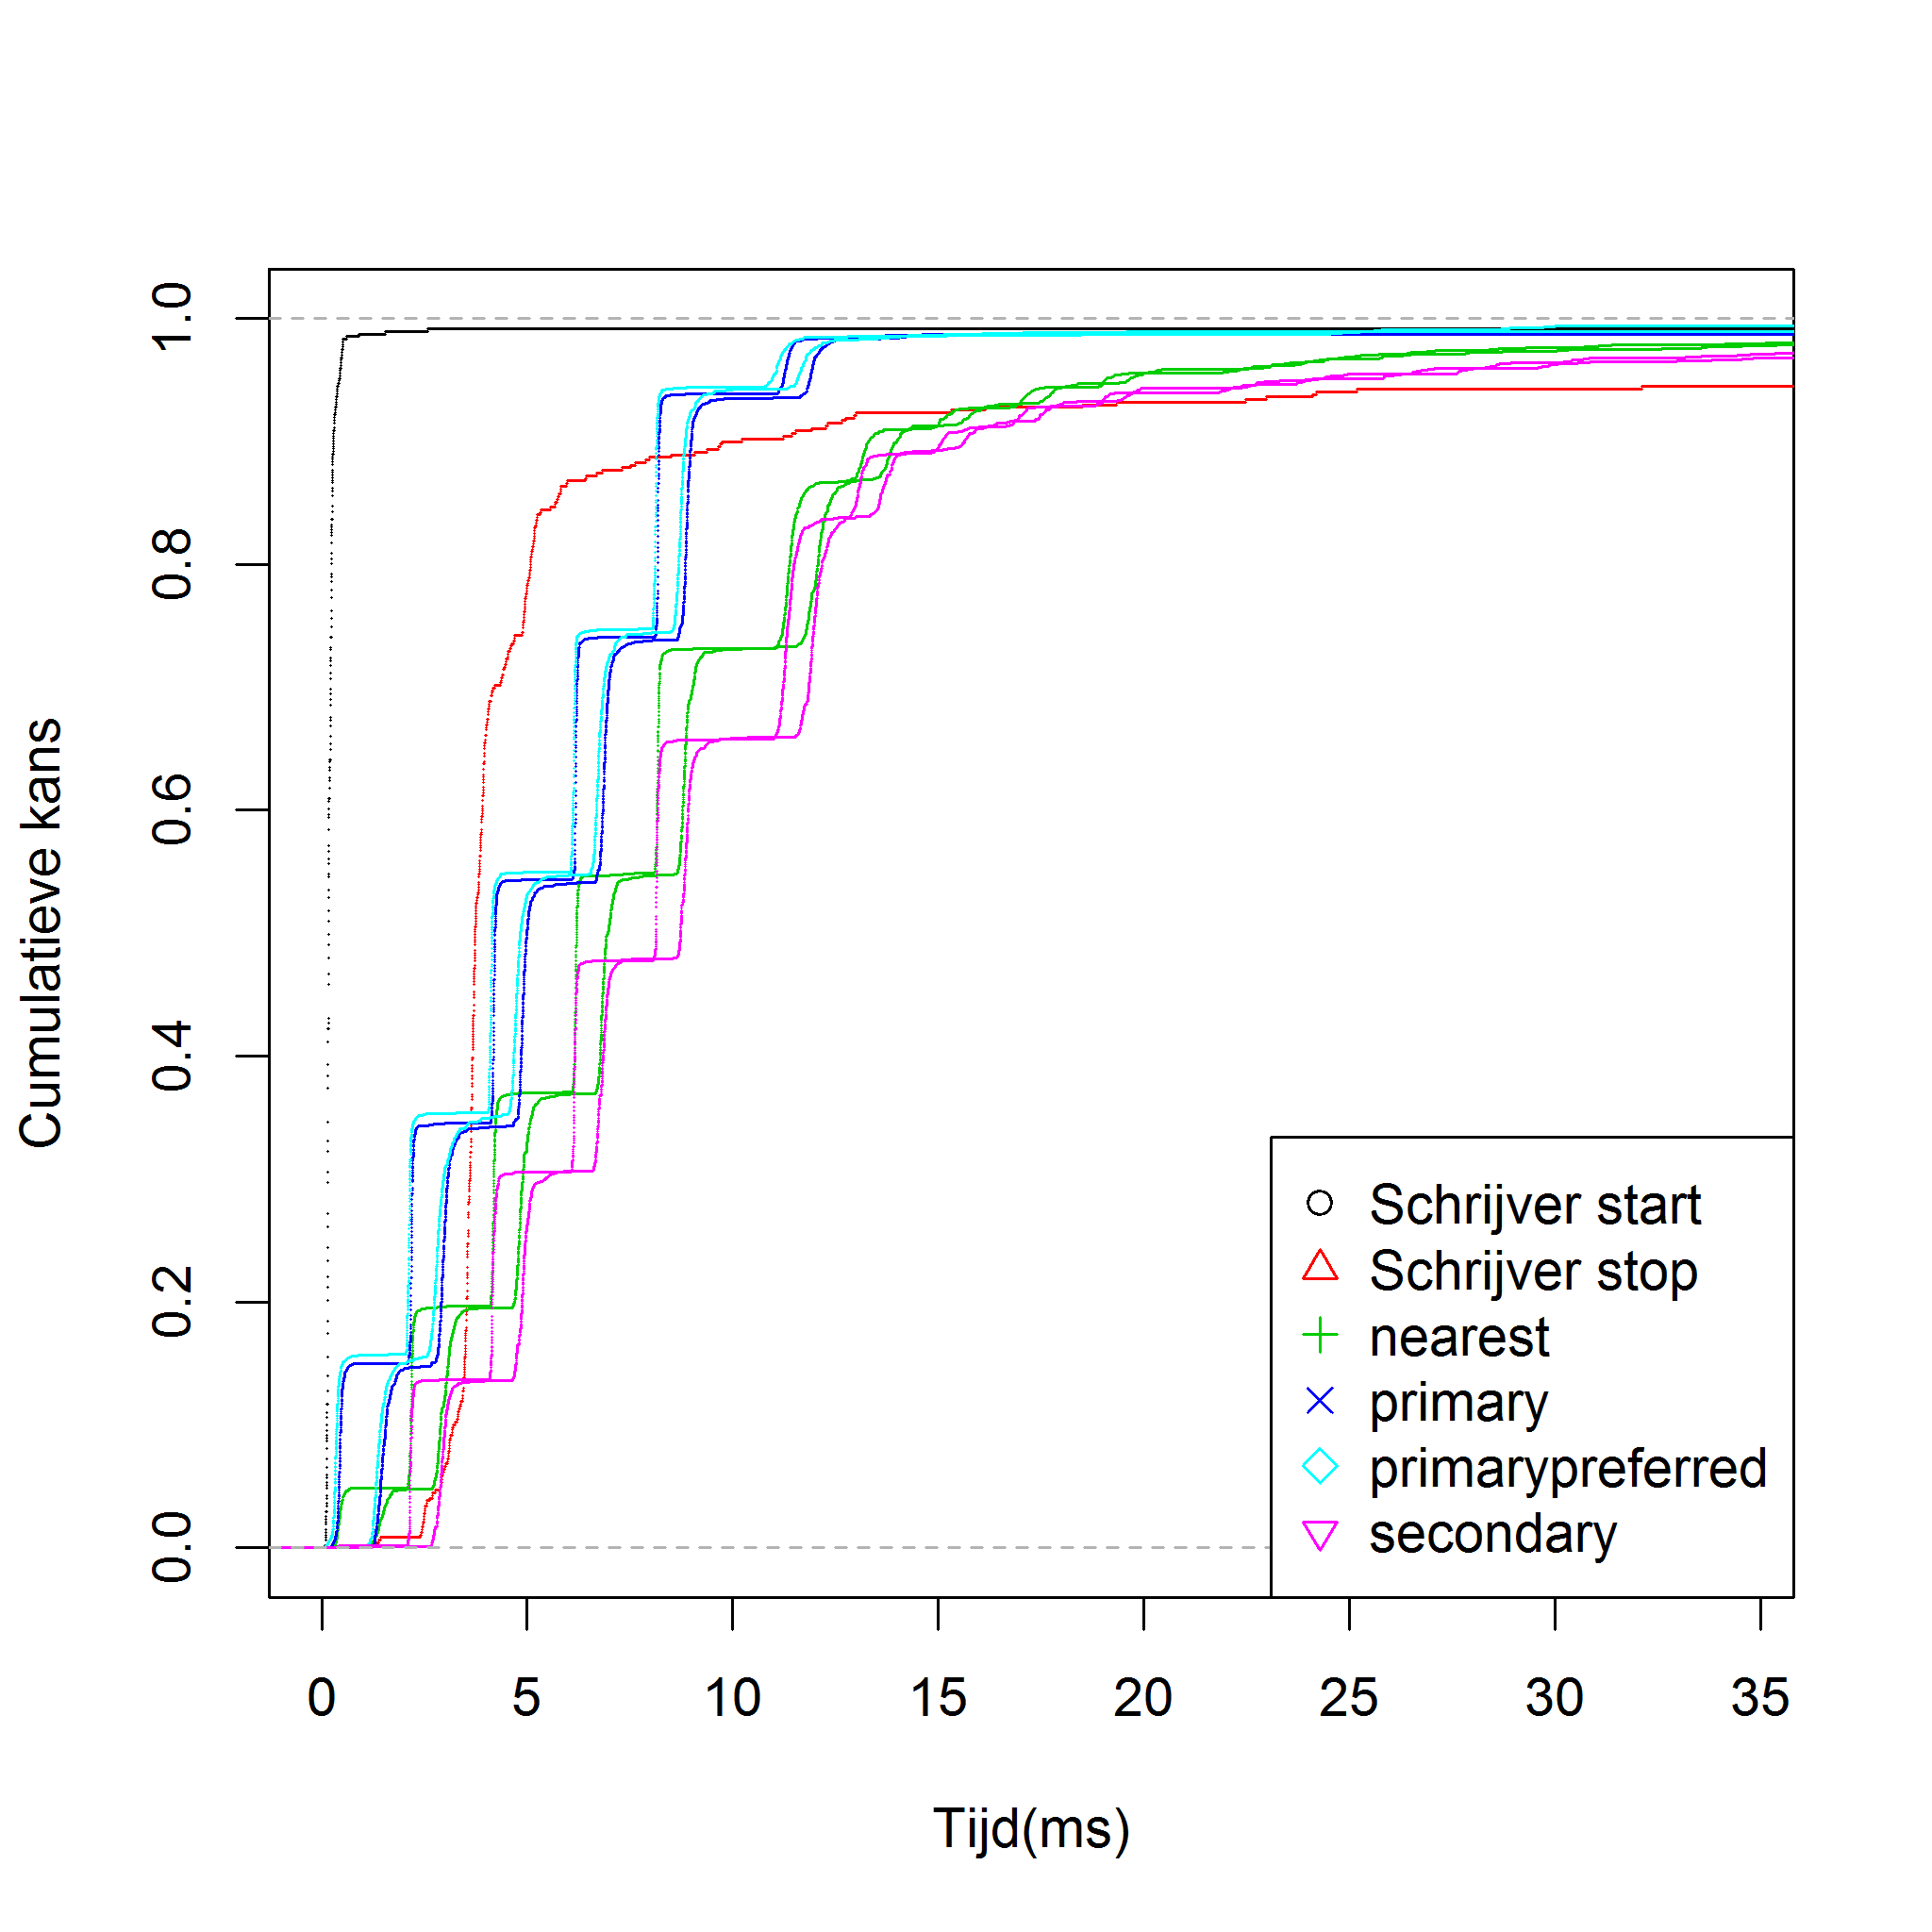
\includegraphics[width=.42\textwidth]{img/Observaties/MongoDB/ECDF-Reads-update-replicas_safe-all-2}}
	\subfigure[Majority Update]{\label{fig:consistentie-mongodb-all-majority} 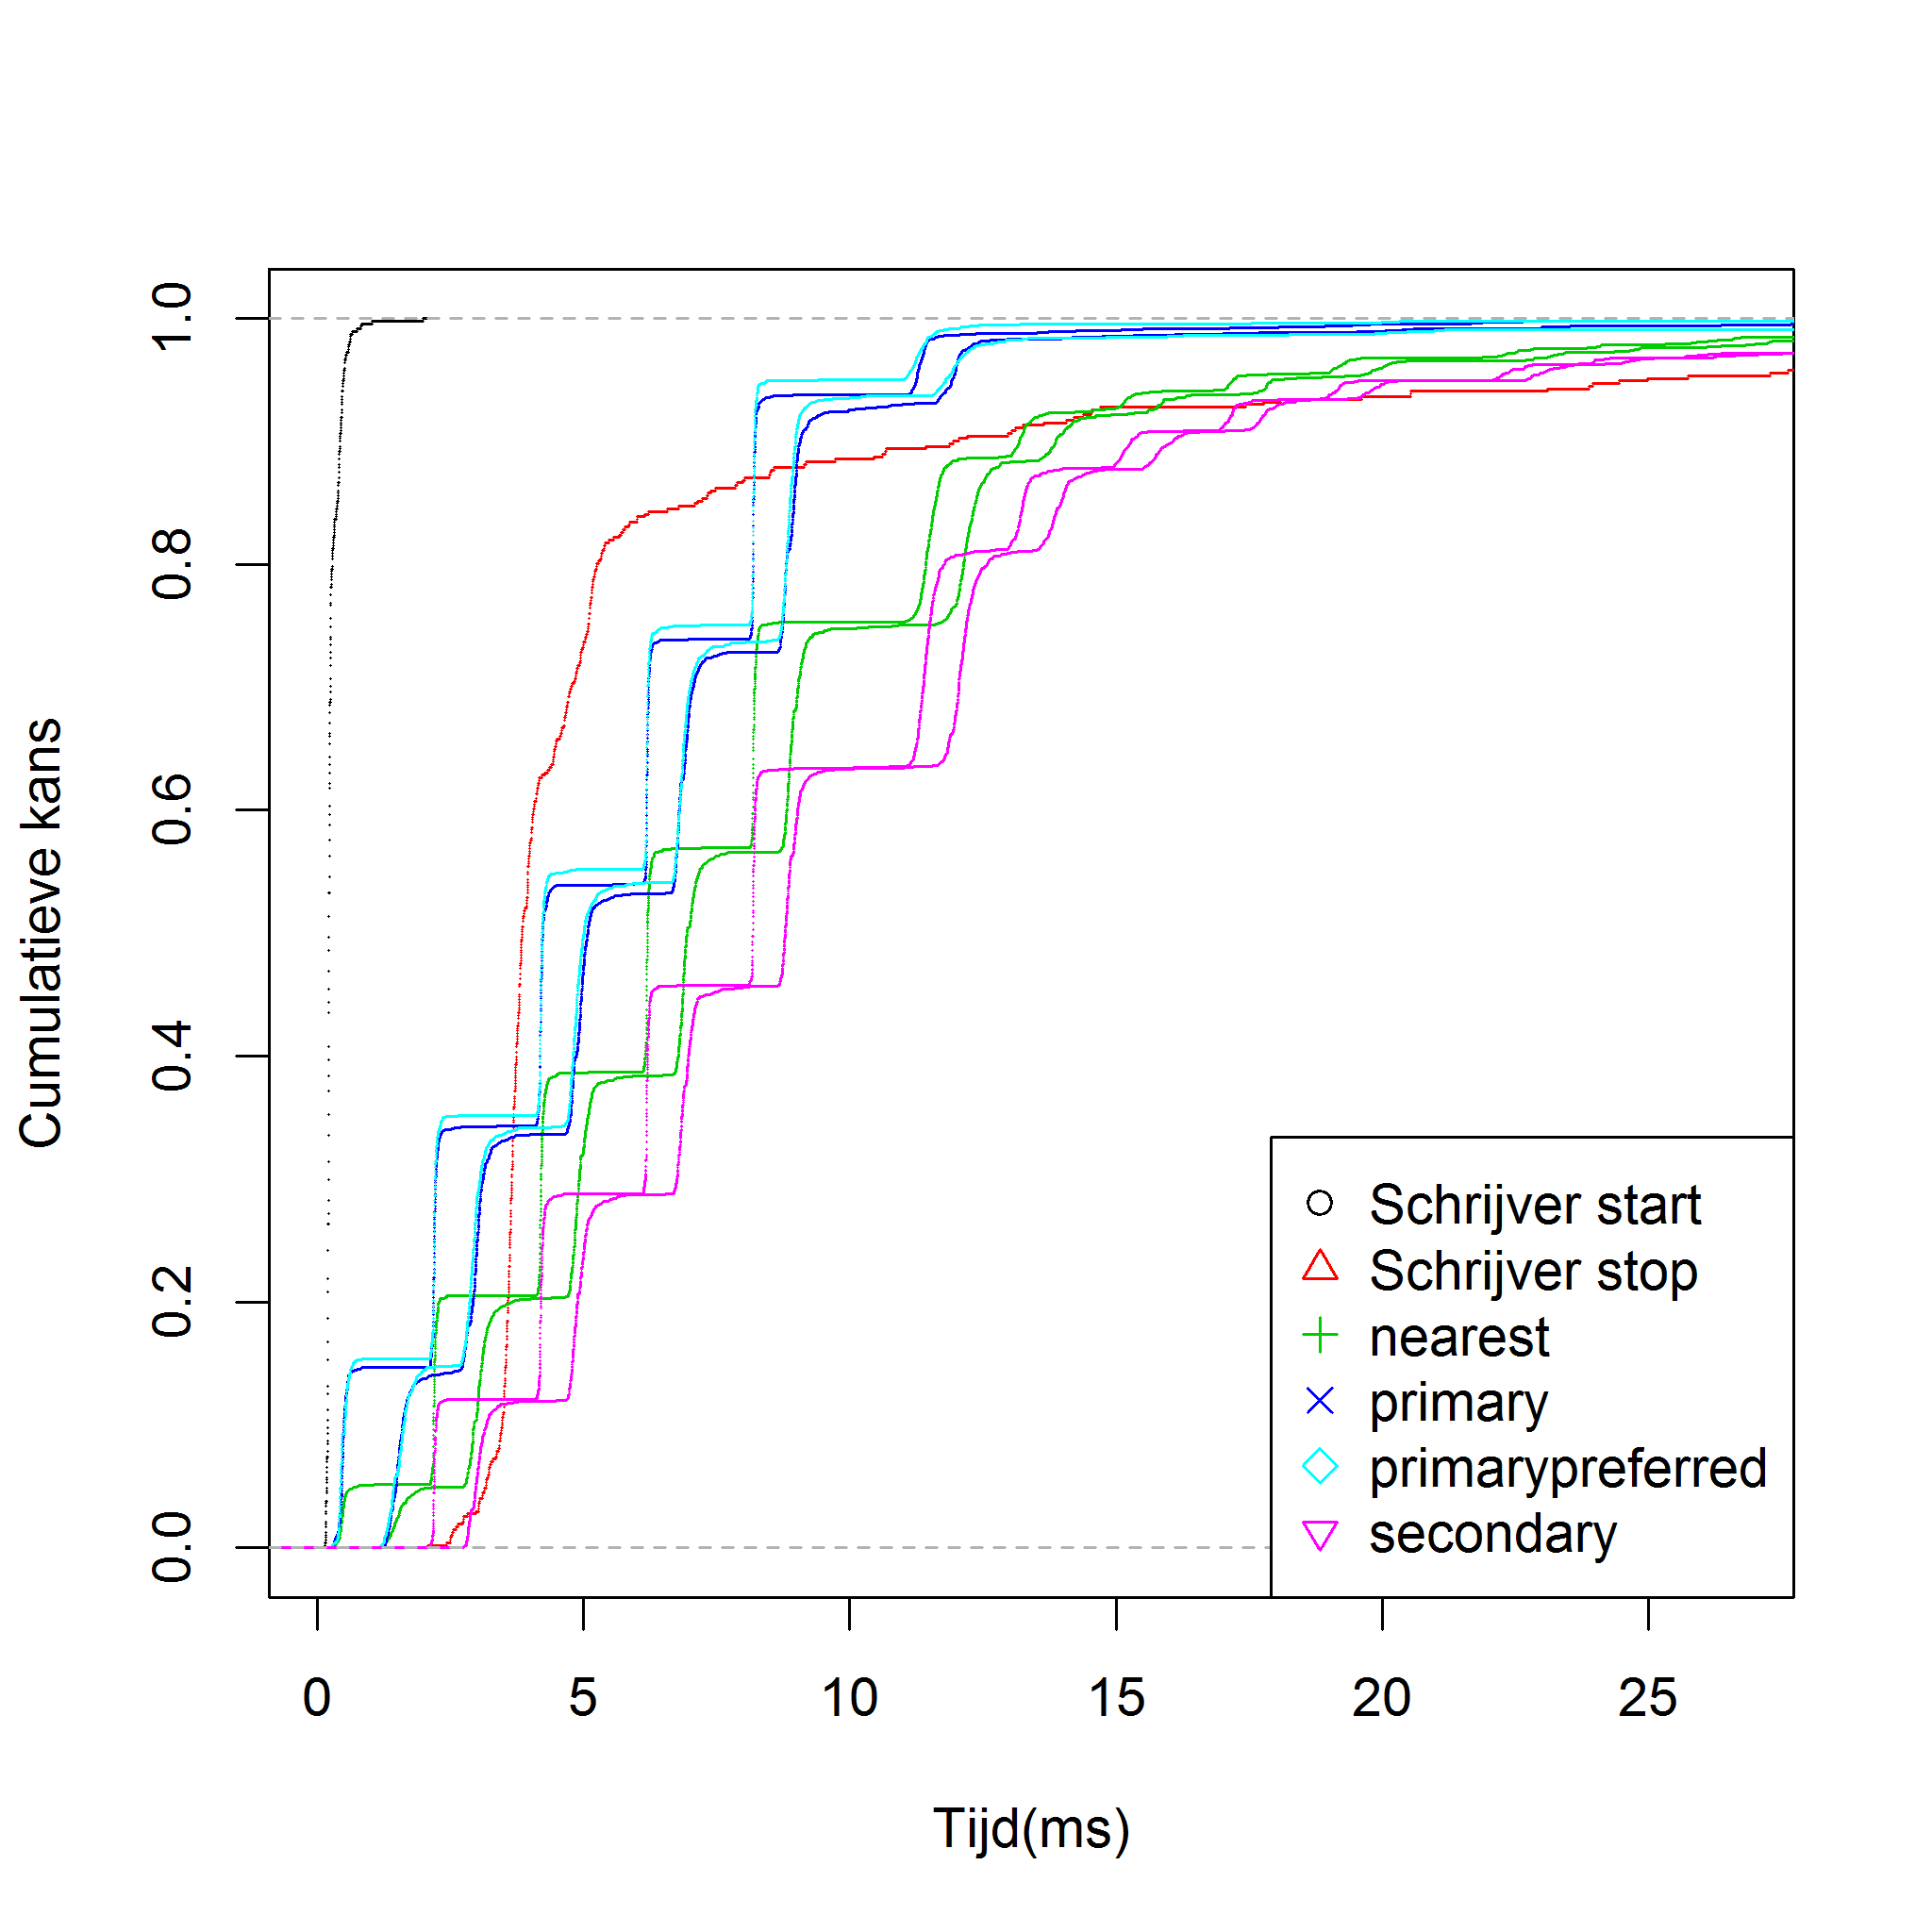
\includegraphics[width=.42\textwidth]{img/Observaties/MongoDB/ECDF-Reads-update-majority-all-2}}
	\subfigure[Majority Insert]{\label{fig:consistentie-mongodb-all-majority-insert} 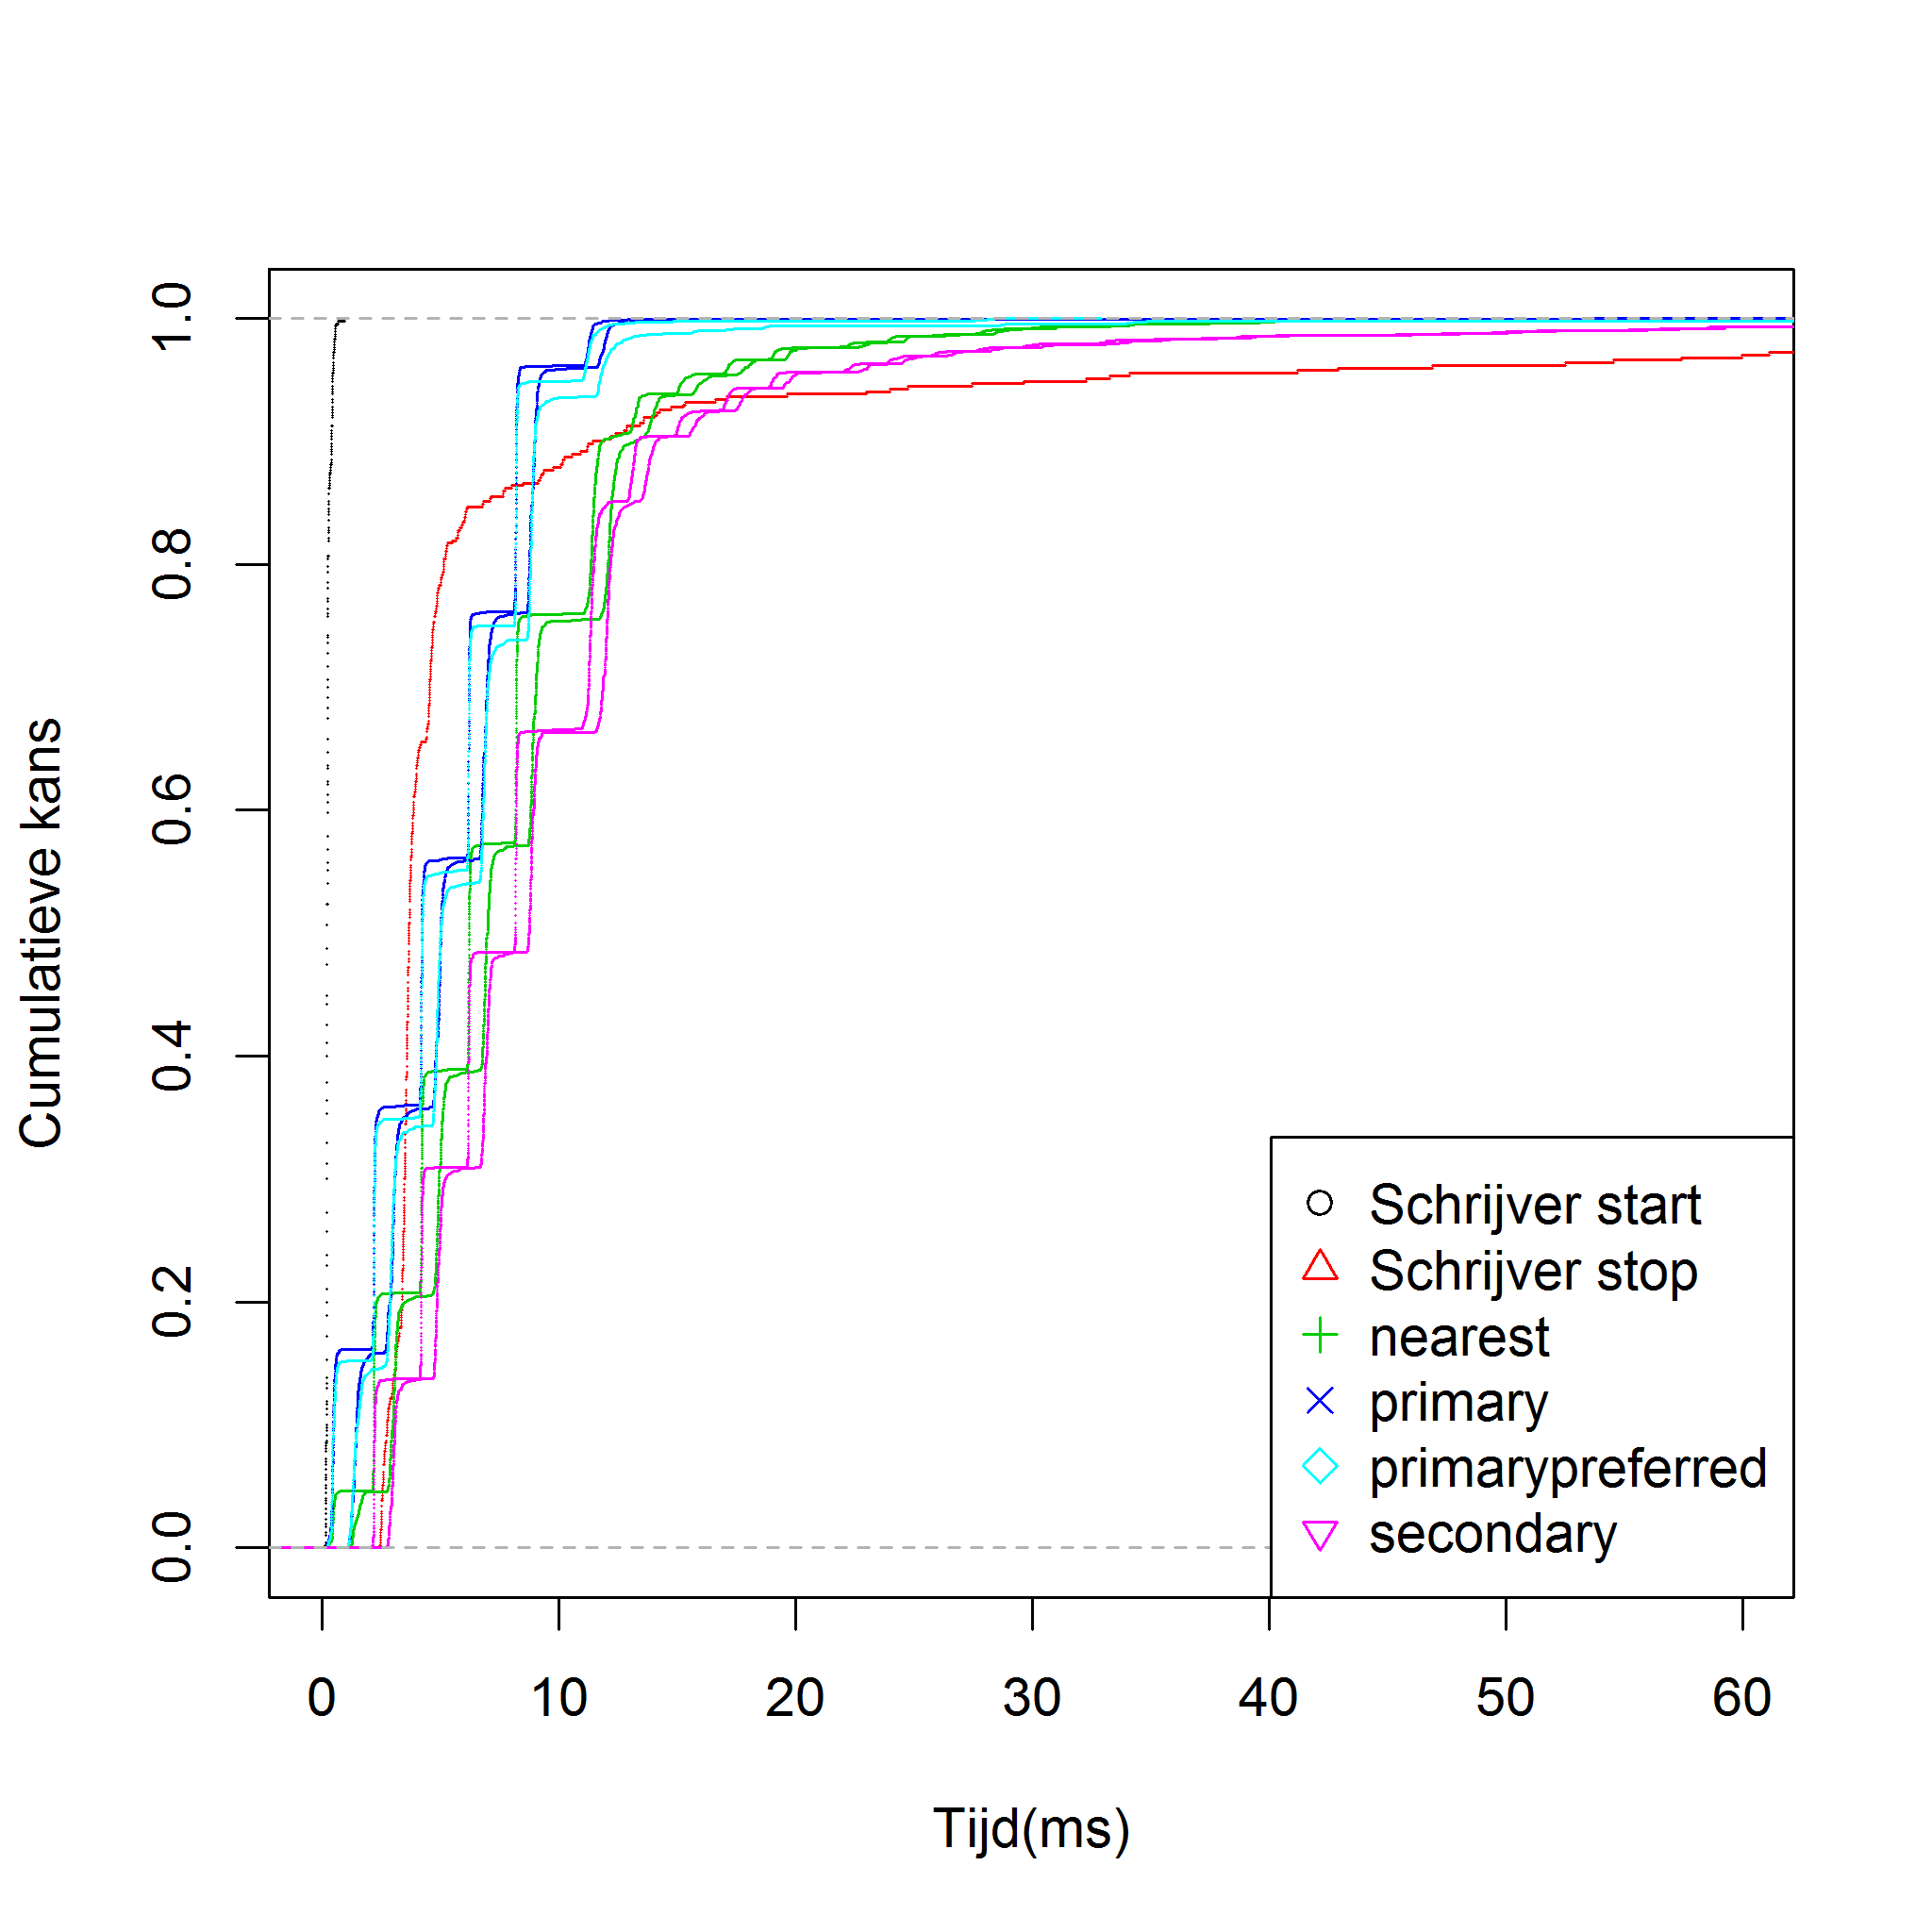
\includegraphics[width=.42\textwidth]{img/Observaties/MongoDB/ECDF-Reads-insert-majority-all-2}}
	\caption{Consistentie: Overzicht van MongoDB op de consistentie testen voor alle lezers gecombineerd met een 97-percentiel }
	\label{fig:consistentie-mongodb-all}
\end{figure}

\begin{figure}[ht!] 
	\centering
	\subfigure[Normal Update]{\label{fig:consistentie-mongodb-R2-normal} 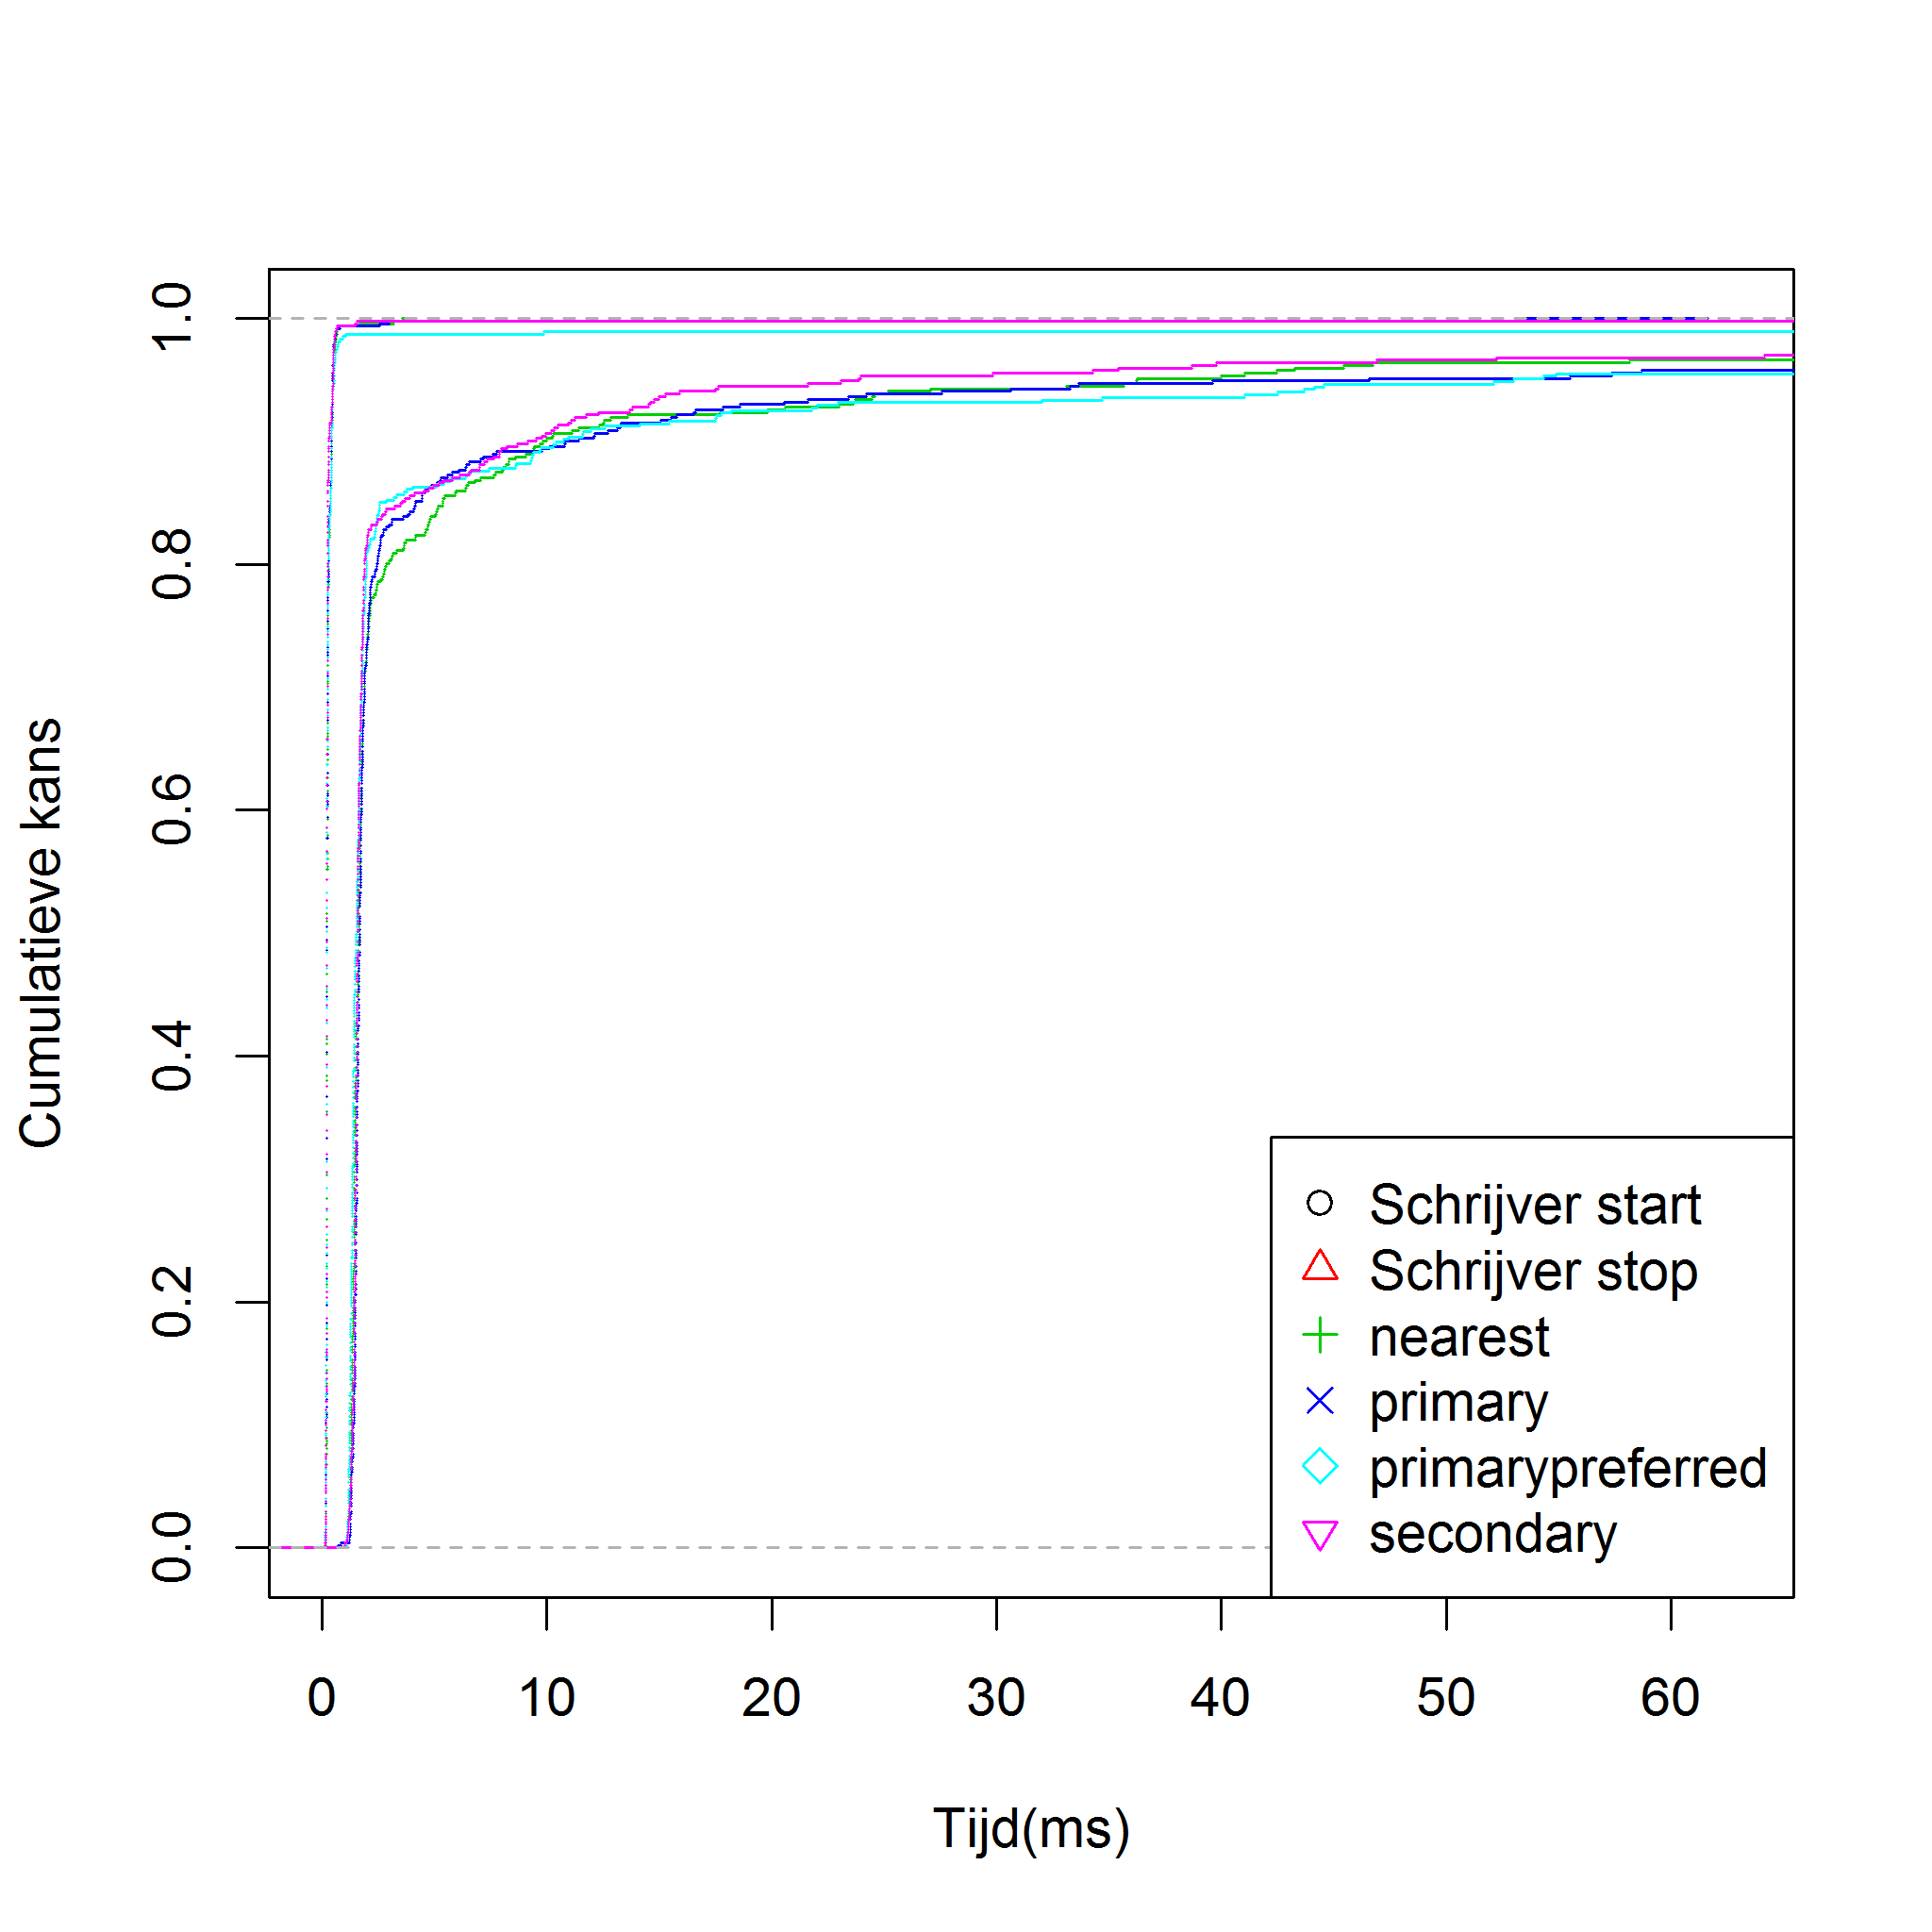
\includegraphics[width=.42\textwidth]{img/Observaties/MongoDB/ECDF-Reads-update-normal-1-2}}
	\subfigure[Safe Update]{\label{fig:consistentie-mongodb-R2-safe} 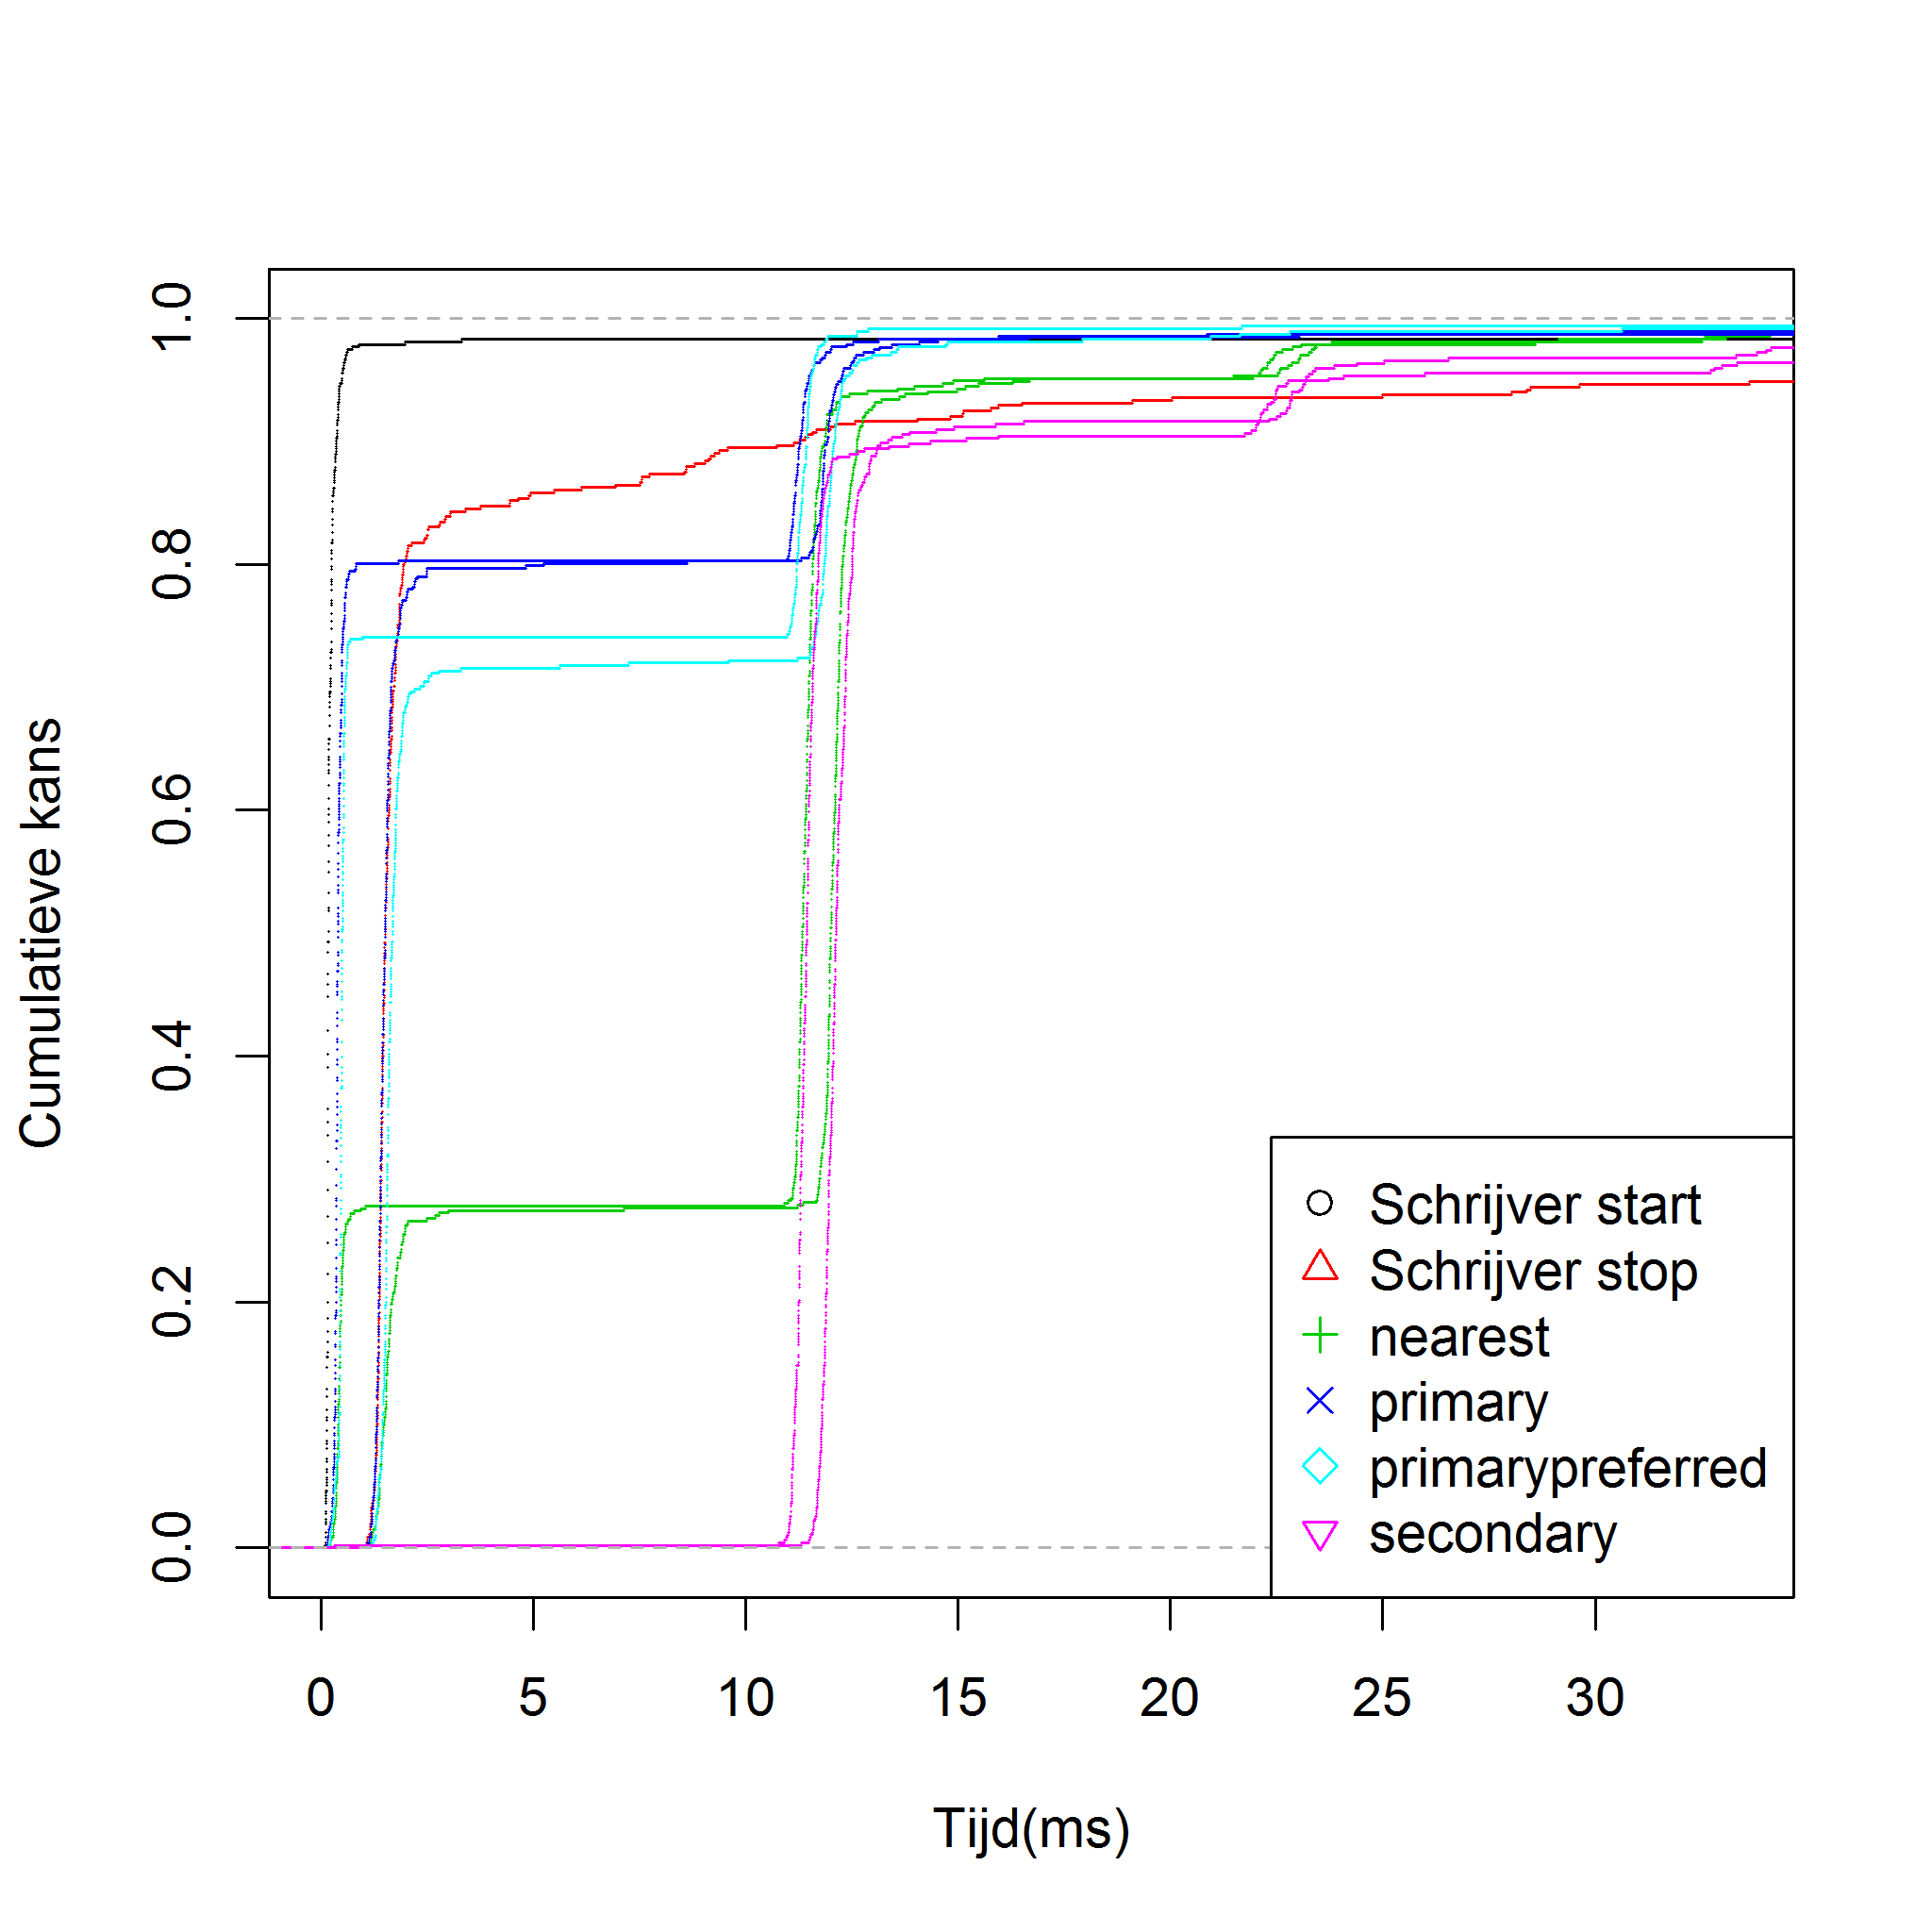
\includegraphics[width=.42\textwidth]{img/Observaties/MongoDB/ECDF-Reads-update-safe-1-2}}
	\subfigure[Fsync Safe Update]{\label{fig:consistentie-mongodb-R2-fsync} 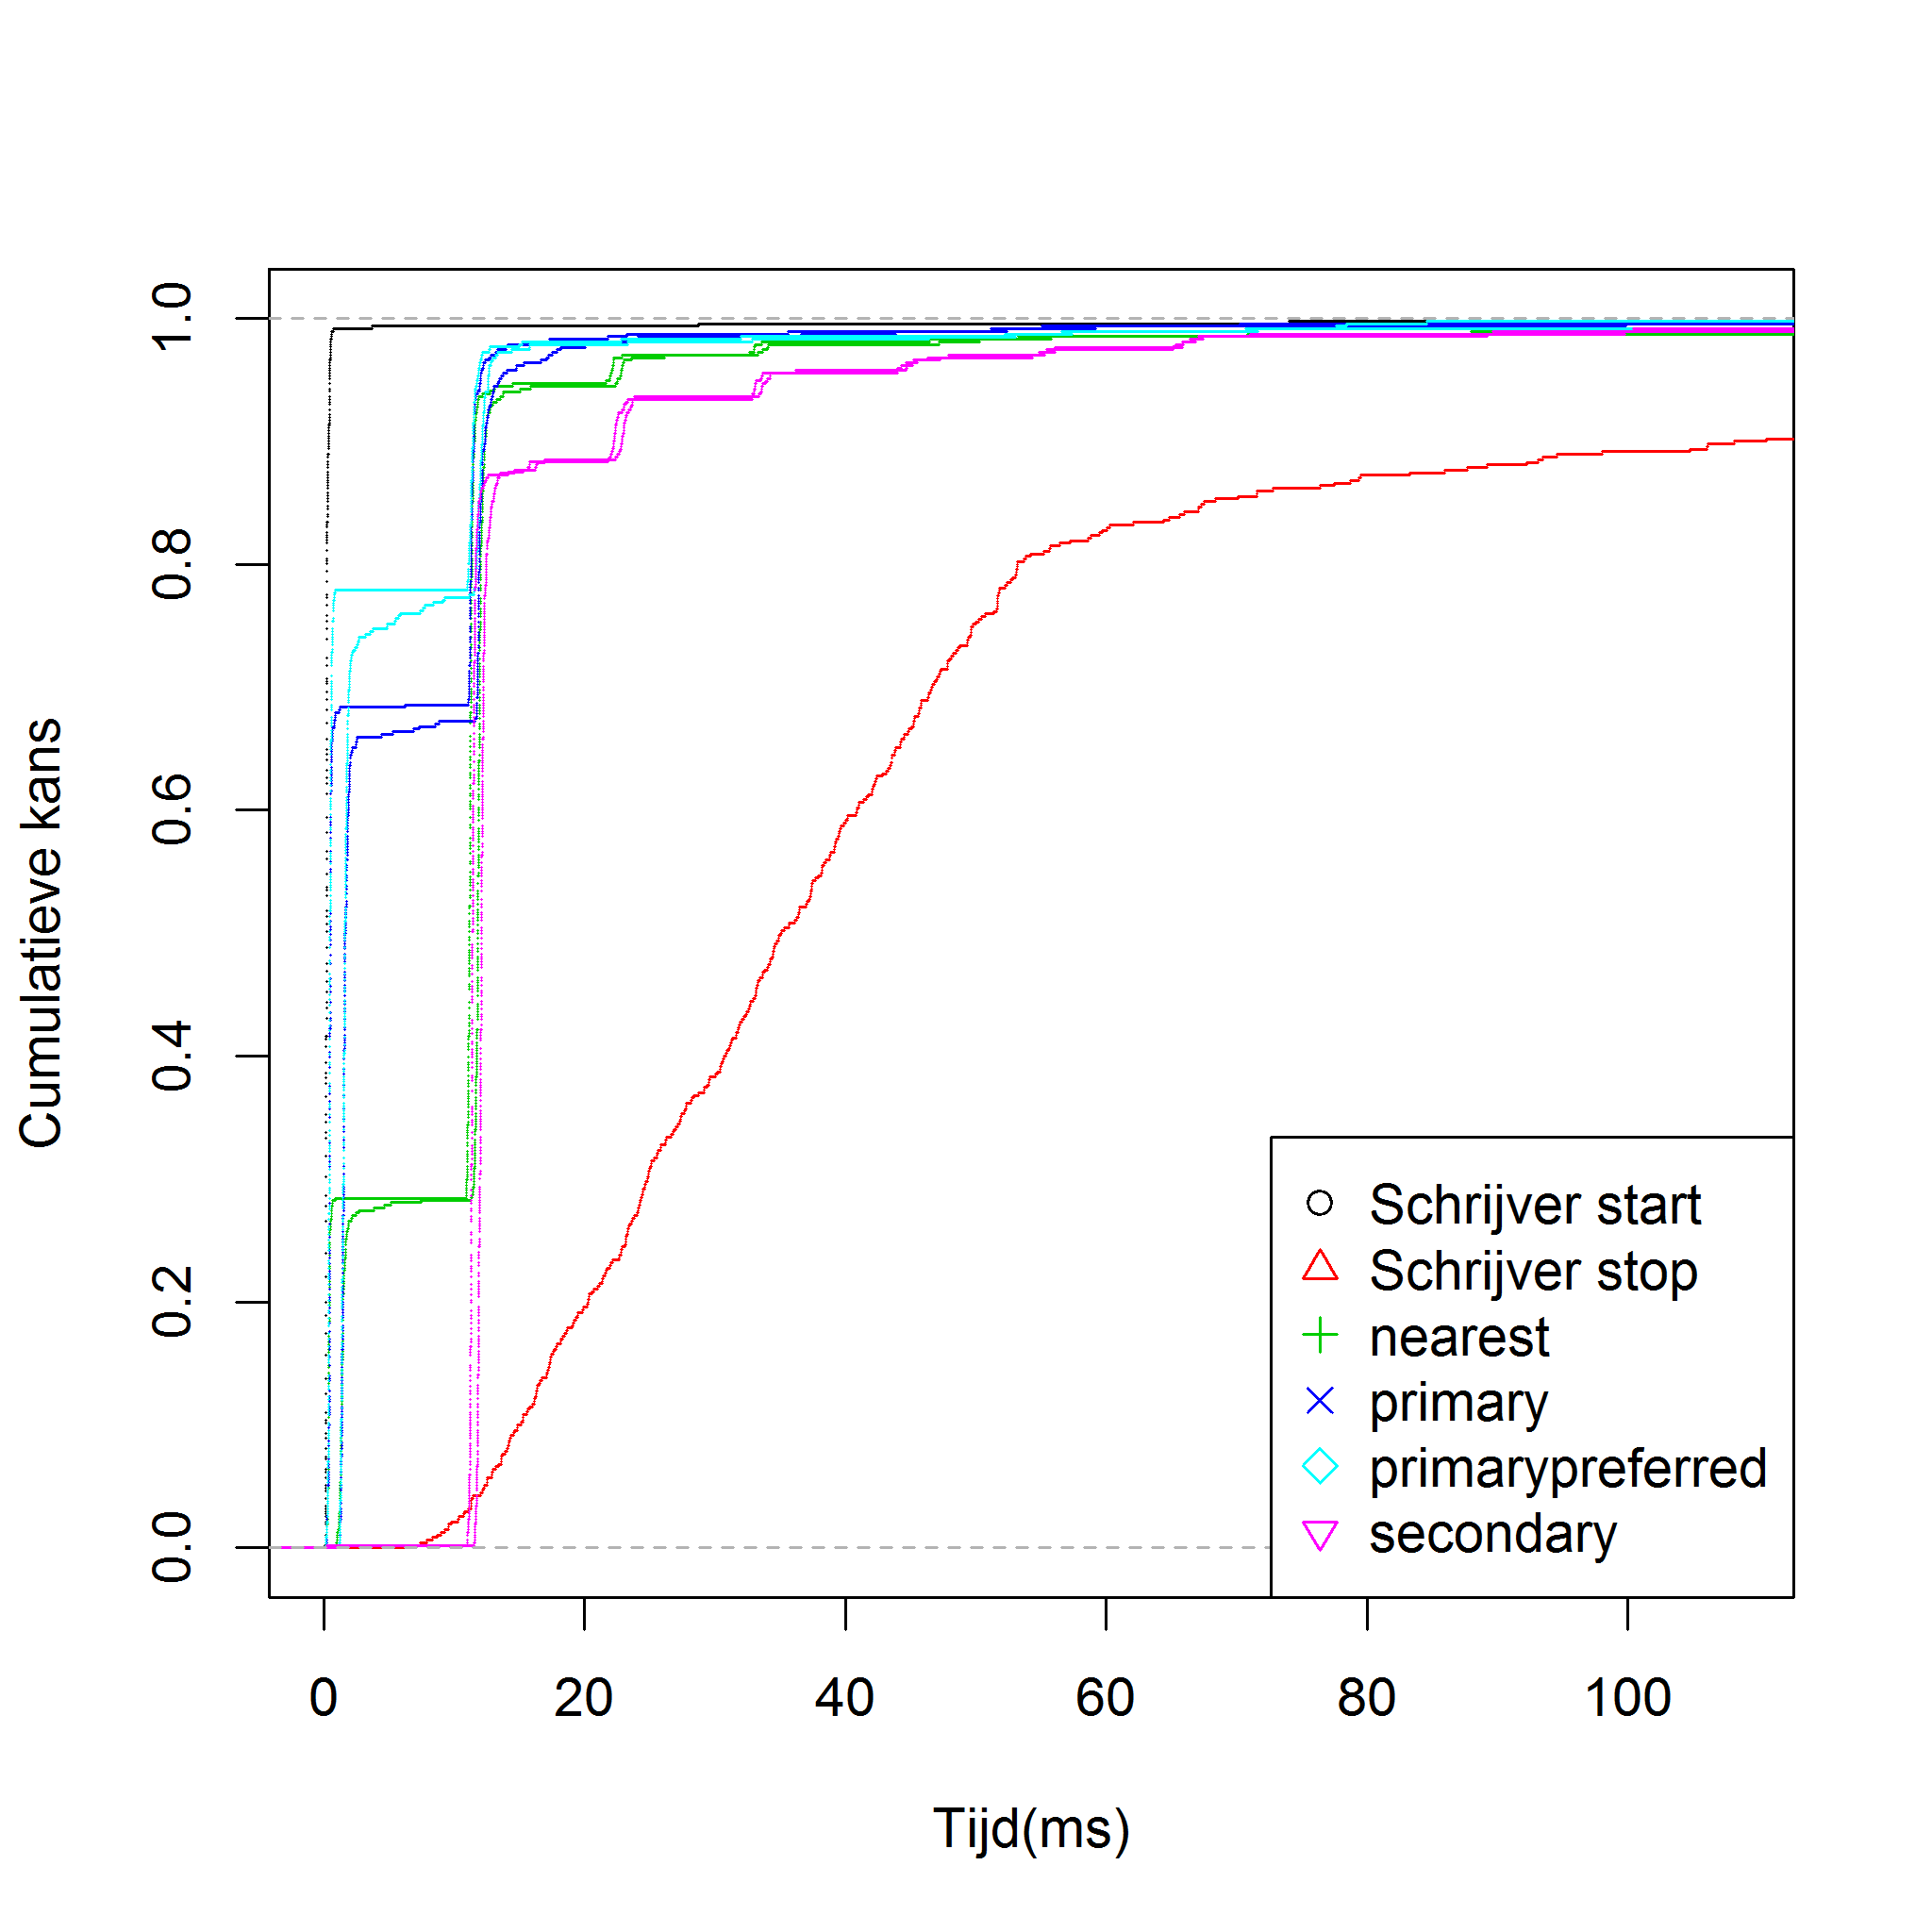
\includegraphics[width=.42\textwidth]{img/Observaties/MongoDB/ECDF-Reads-update-fsync_safe-1-2}}
	\subfigure[Replica Safe Update]{\label{fig:consistentie-mongodb-R2-replicasafe} 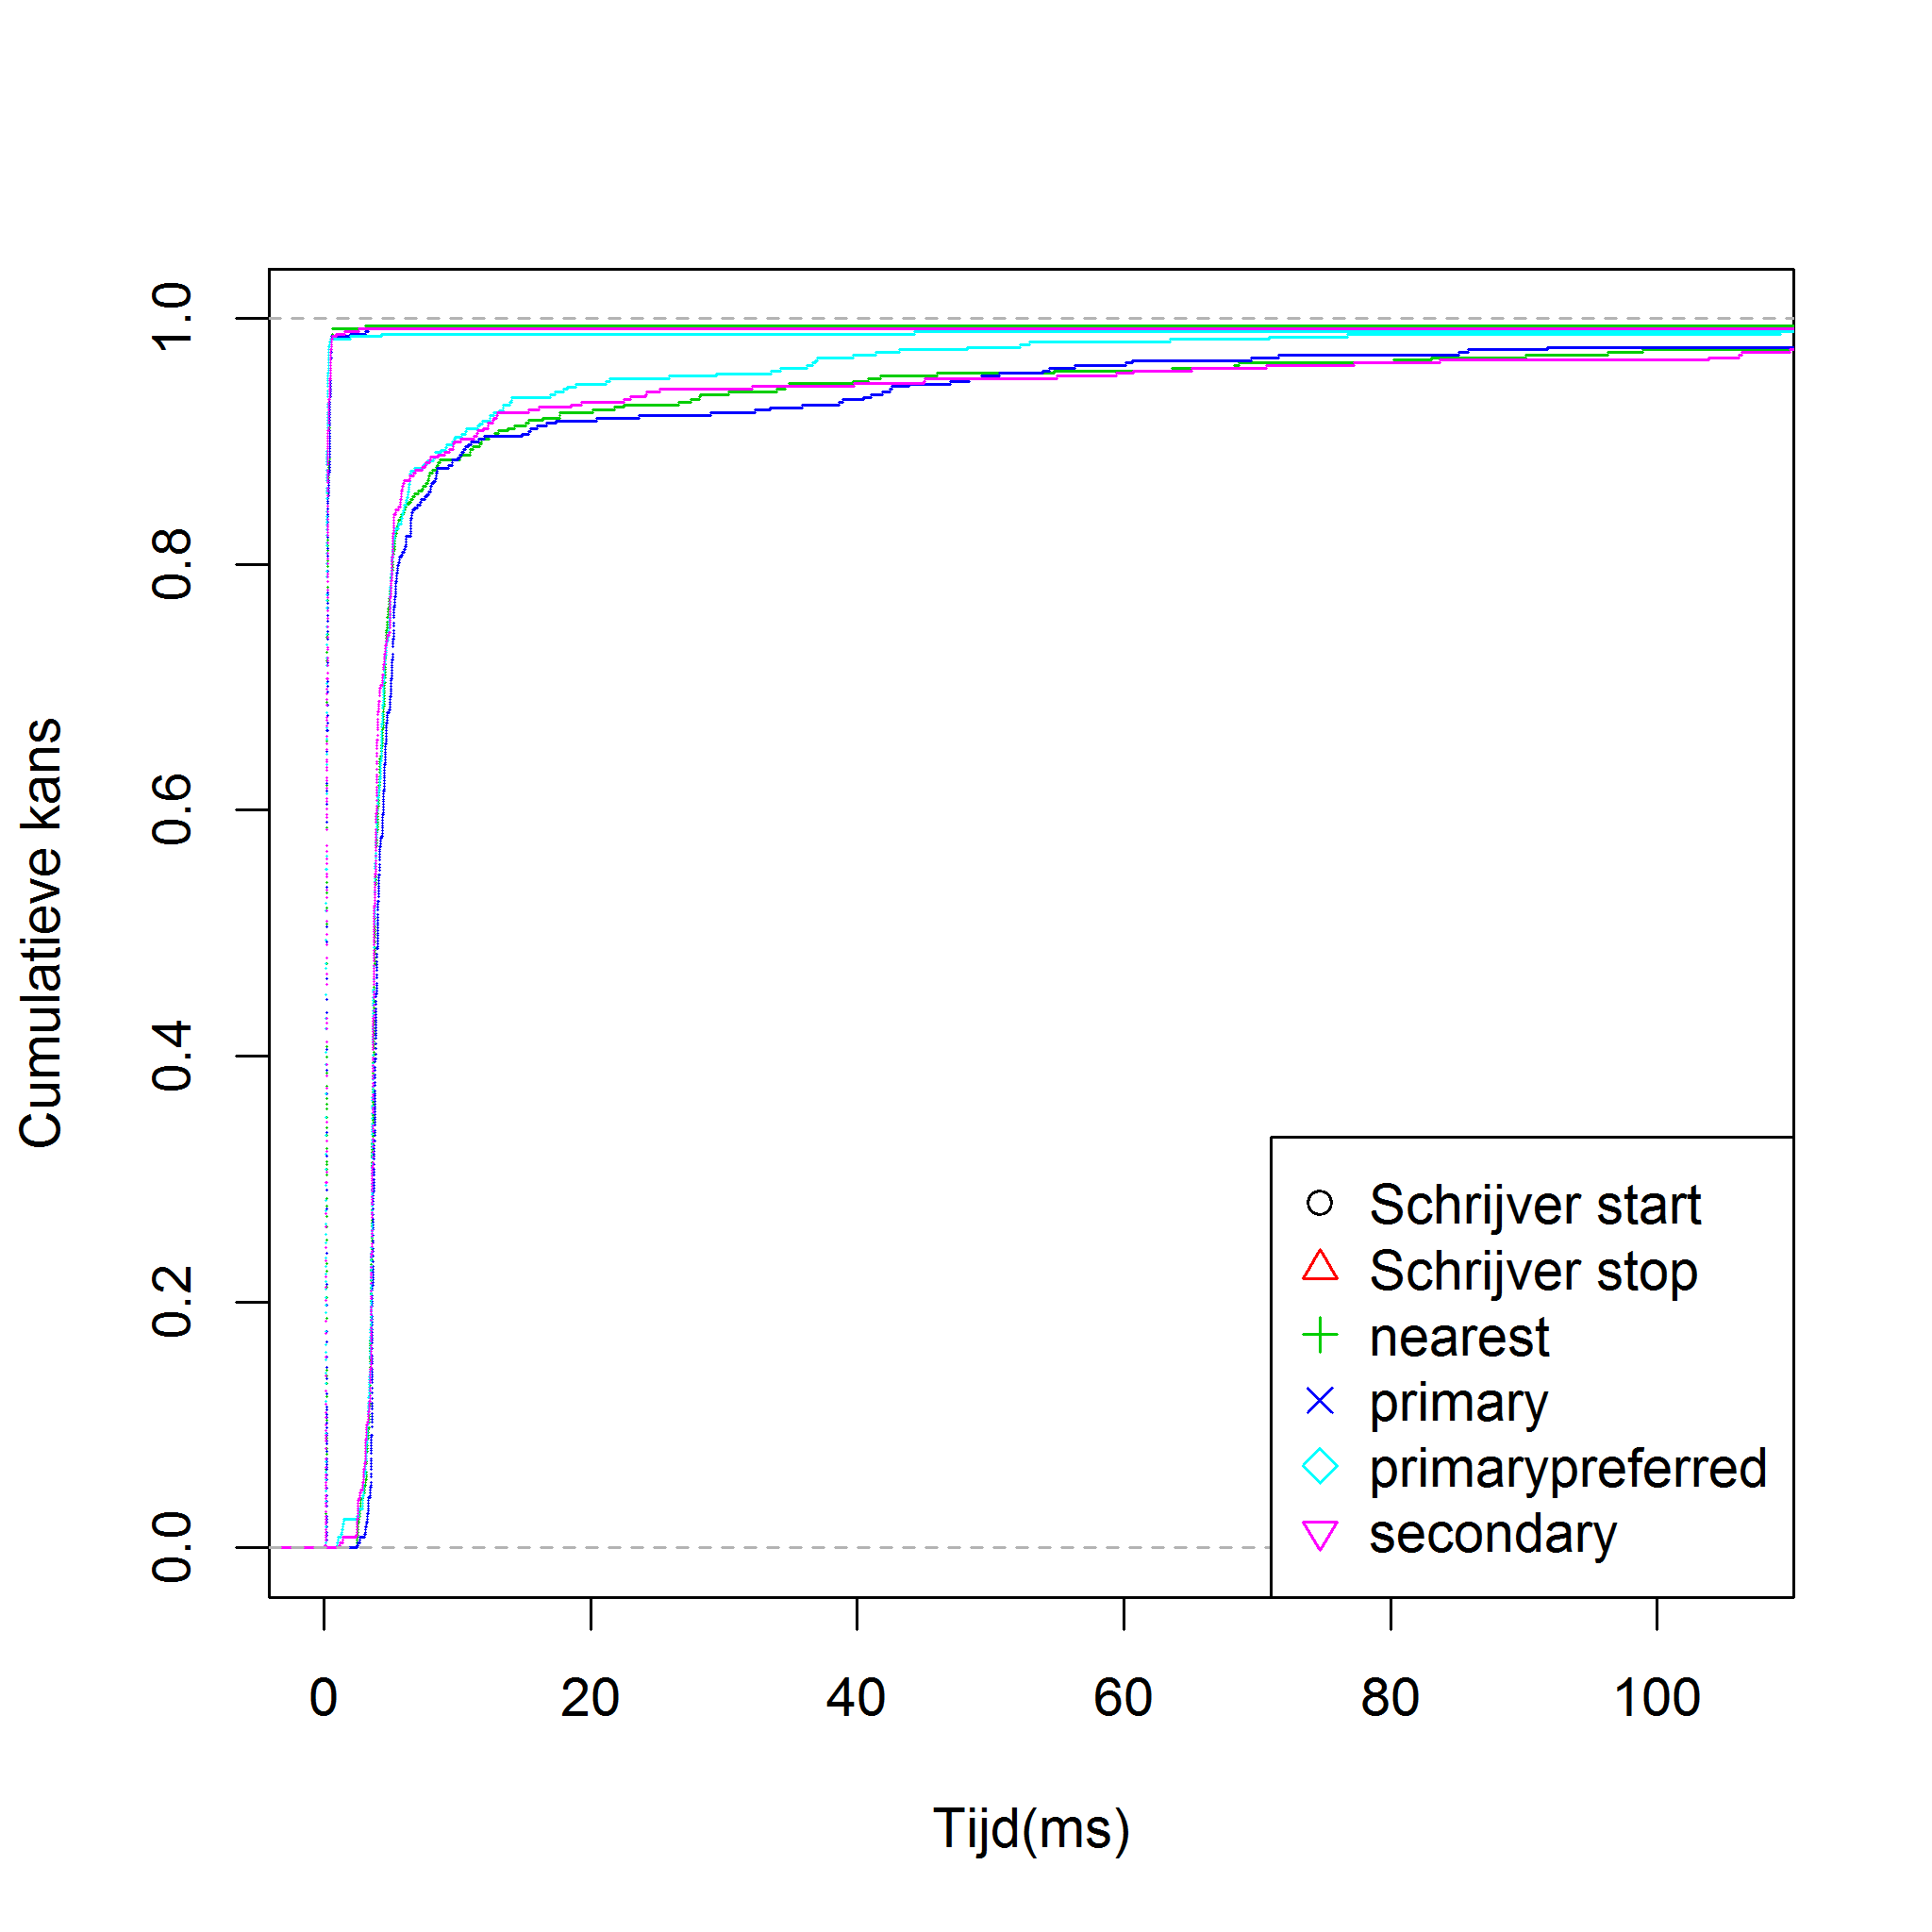
\includegraphics[width=.42\textwidth]{img/Observaties/MongoDB/ECDF-Reads-update-replicas_safe-1-2}}
	\subfigure[Majority Update]{\label{fig:consistentie-mongodb-R2-majority} 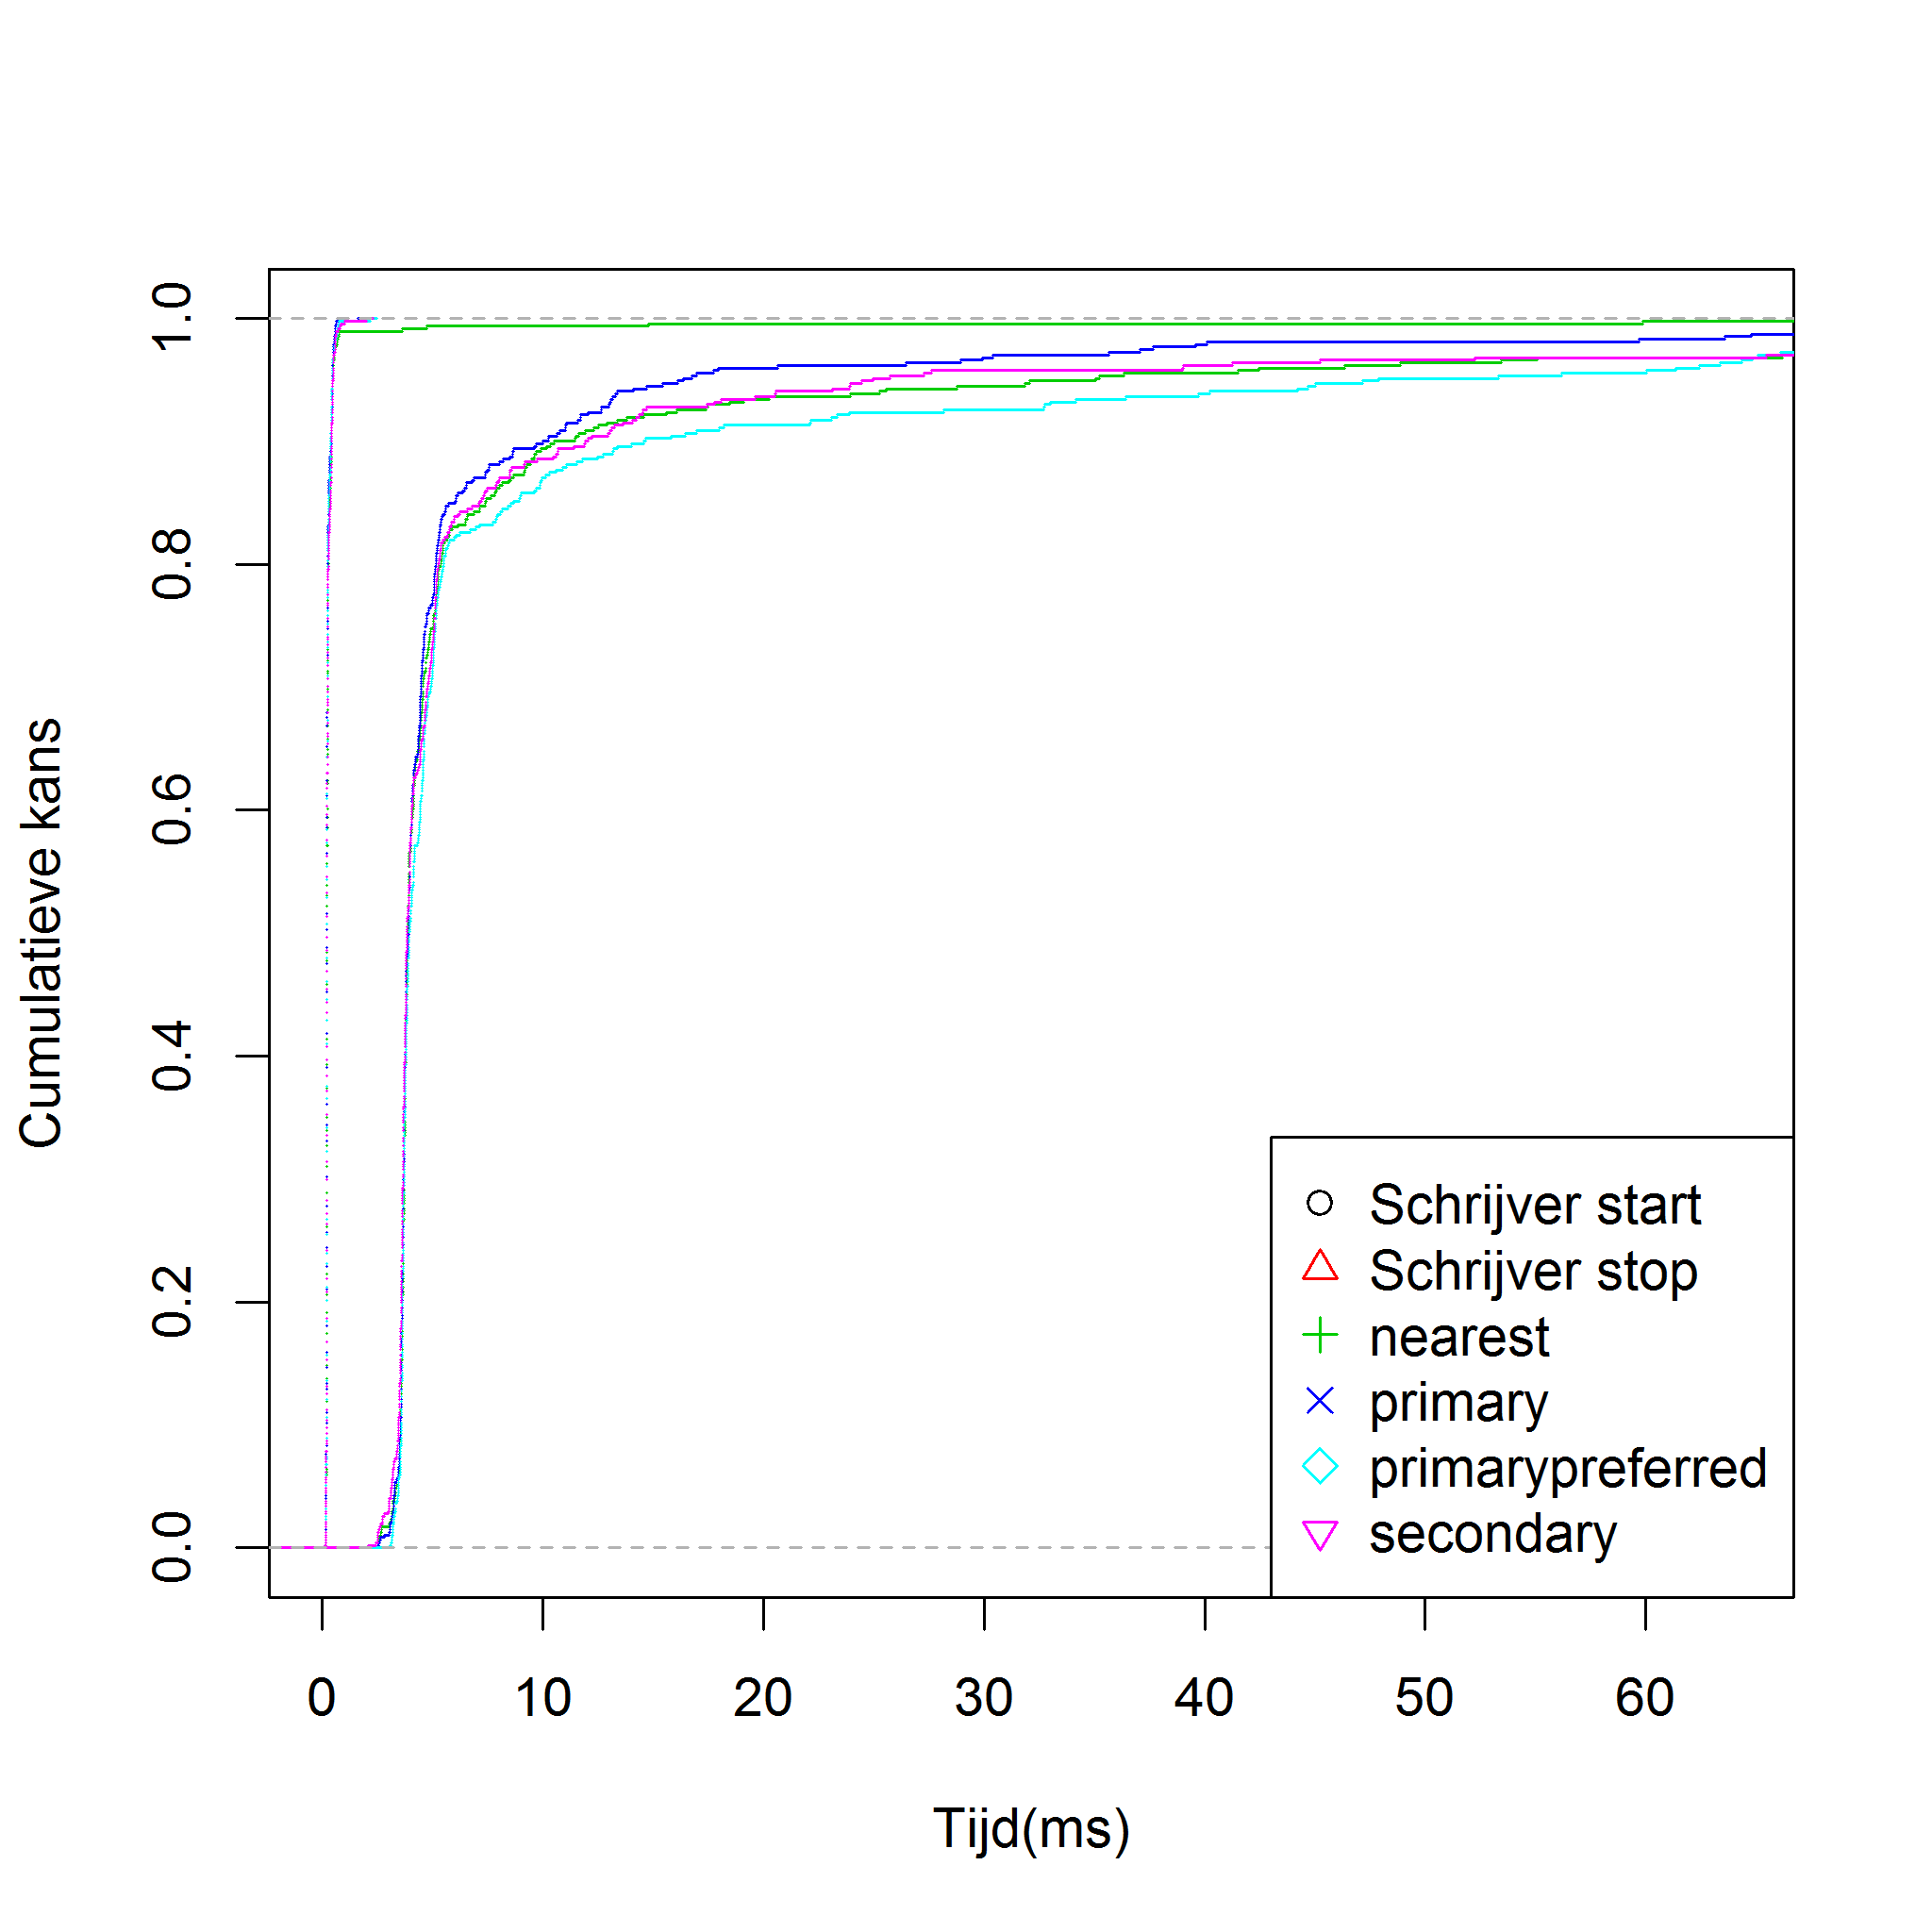
\includegraphics[width=.42\textwidth]{img/Observaties/MongoDB/ECDF-Reads-update-majority-1-2}}
	\subfigure[Majority Insert]{\label{fig:consistentie-mongodb-R2-majority-insert} 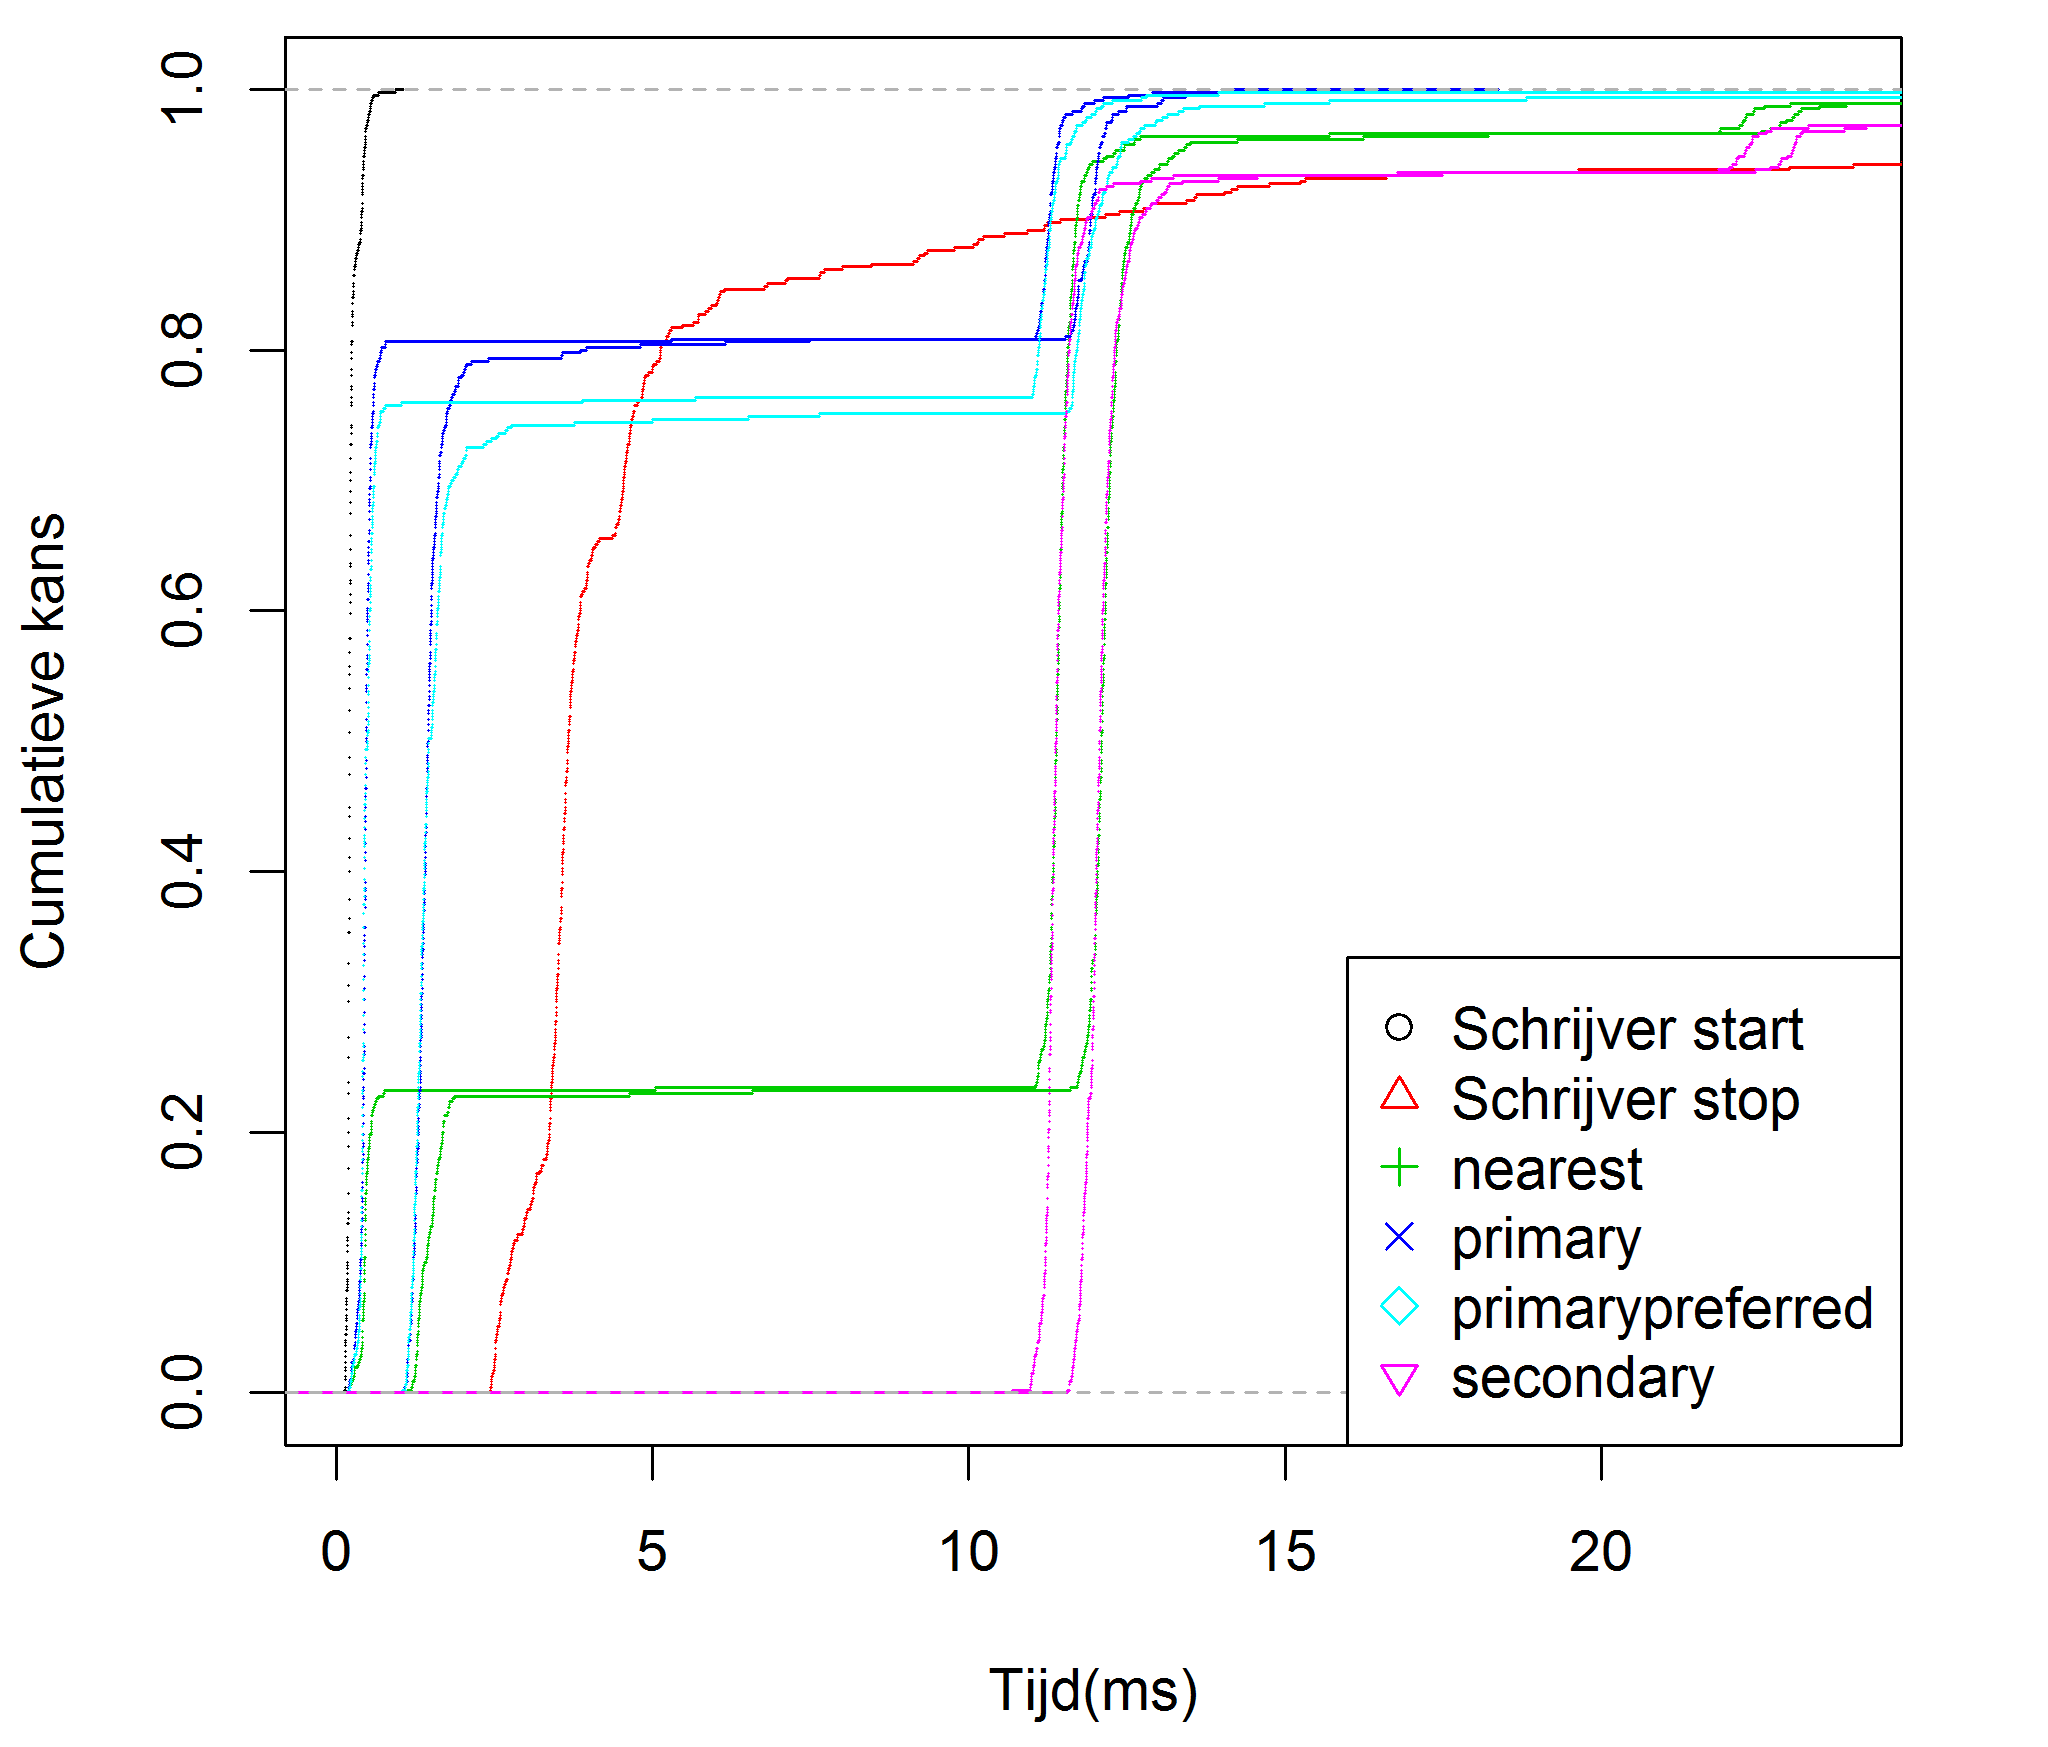
\includegraphics[width=.42\textwidth]{img/Observaties/MongoDB/ECDF-Reads-insert-majority-1-2}}
	\caption{Consistentie: Overzicht van MongoDB op de consistentie testen voor lezer 2 met een 99-percentiel}
	\label{fig:consistentie-mongodb-R2}
\end{figure}

\section{Conclusie}
Uit de testen 
